%%%%% Single page layout:
%%%%% ----------------------------------------------------
\documentclass[12pt, a4paper]{report}
\setlength\textwidth{160mm}
\setlength\textheight{247mm}
\setlength\oddsidemargin{0mm}
\setlength\evensidemargin{0mm}
\setlength\topmargin{0mm}
\setlength\headsep{0mm}
\setlength\headheight{0mm}
\let\openright=\clearpage
\usepackage[utf8]{inputenc}

%%% Additional useful packages
%%% ----------------------------------------------------------------
\usepackage{array}
\usepackage{amsmath}  
\usepackage{amssymb}
\usepackage{amsfonts}
\DeclareFontFamily{OT1}{pzc}{}
\DeclareFontShape{OT1}{pzc}{m}{it}{<-> s * [0.900] pzcmi7t}{}
\DeclareMathAlphabet{\mathpzc}{OT1}{pzc}{m}{it}
\usepackage{amsthm}      
\usepackage{algorithm2e}
\usepackage{algorithmic}
\usepackage{bm}
\usepackage[mathscr]{euscript}
\usepackage{graphicx}       
\usepackage{psfrag}         
\usepackage{fancyvrb}    
\usepackage{float}
\usepackage[square,sort,comma,numbers]{natbib}        
\usepackage{bbding}         
\usepackage{dcolumn}        
\usepackage{booktabs} 
\usepackage{multirow}
\usepackage{paralist}       
\usepackage{indentfirst}    
\usepackage[nottoc,notlof,notlot]{tocbibind}
\usepackage{url}
\usepackage{tabularx}
\usepackage{subcaption}
\usepackage[unicode]{hyperref}
\hypersetup{pdftitle=LiDAR obstacle detection and avoidance, 
            pdfauthor=Alojz Gomola,
            colorlinks=false,
            urlcolor=blue,
            pdfstartview=FitH,
            pdfpagemode=UseOutlines,
            pdfnewwindow,
            breaklinks
          }
\usepackage{array}
\newcolumntype{L}[1]{>{\raggedright\let\newline\\\arraybackslash\hspace{0pt}}m{#1}}
\newcolumntype{C}[1]{>{\centering\let\newline\\\arraybackslash\hspace{0pt}}m{#1}}
\newcolumntype{R}[1]{>{\raggedleft\let\newline\\\arraybackslash\hspace{0pt}}m{#1}}         

\newcommand{\FIGDIR}{./Pics}    %%% directory containing figures
\newcommand{\twolinecellr}[2][r]{%
  \begin{tabular}[#1]{@{}r@{}}#2\end{tabular}}
\theoremstyle{plain}
\newtheorem{theorem}{Theorem}
\newtheorem{lemma}[theorem]{Lemma}
\newtheorem{proposition}[theorem]{Proposition}

\theoremstyle{plain}
\newtheorem{definition}{Definition}
\newtheorem{problem}{Problem}
\newtheorem{example}{Example}
\newtheorem{assumption}{Assumption}

\theoremstyle{remark}
\newtheorem*{corollary}{Corollary}
\newtheorem*{note}{Note}



\newenvironment{dokaz}{
  \par\medskip\noindent
  \textit{Proof}.
}{
\newline
\rightline{\SquareCastShadowBottomRight}
}


%\bibliographystyle{plainnat}     %% Author (year) style
\bibliographystyle{unsrt}        %% [number] style
\setcitestyle{square}


\title{FEUP research plan}
\author{Alojz Gomola}
\date{May 2016}

%%%%% ------------------------------------------------------------
\DefineVerbatimEnvironment{PCinout}{Verbatim}{fontsize=\small, frame=single}



\newcommand{\R}{\mathbb{R}}
\newcommand{\N}{\mathbb{N}}

\DeclareMathOperator{\pr}{\textsf{P}}
\DeclareMathOperator{\E}{\textsf{E}\,}
\DeclareMathOperator{\var}{\textrm{var}}
\DeclareMathOperator{\sd}{\textrm{sd}}


\newcommand{\T}[1]{#1^\top}        

\newcommand{\goto}{\rightarrow}
\newcommand{\gotop}{\stackrel{P}{\longrightarrow}}
\newcommand{\maon}[1]{o(n^{#1})}
\newcommand{\abs}[1]{\left|{#1}\right|}
\newcommand{\dint}{\int_0^\tau\!\!\int_0^\tau}
\newcommand{\isqr}[1]{\frac{1}{\sqrt{#1}}}
\newcommand{\norm}[1]{\left\lVert#1\right\rVert}


\newcommand{\pulrad}[1]{\raisebox{1.5ex}[0pt]{#1}}
\newcommand{\mc}[1]{\multicolumn{1}{c}{#1}}

\begin{document}

%Title page 
\pagestyle{empty}
\begin{center}

%header
{FACULDADE DE ENGENHARIA DA UNIVERSIDADE DO PORTO}

\vspace{3cm}
{\LARGE\bfseries Model Predictive Control of}
\vspace{0.2cm}\\
{\LARGE\bfseries Unmanned Air Vehicles with}
\vspace{0.2cm}\\
{\LARGE\bfseries Obstacle Avoidance Capabilities}
\vspace{1.2cm}\\
{\LARGE Exam report}

\vspace{1cm}
{\LARGE Alojz Gomola}


\vspace{5cm}
\centerline{\mbox{
\includegraphics[width=60mm]{\FIGDIR/feuplogo.eps}}}


\vspace{2cm}
{\LARGE Doutoramento em Matemática Aplicada}

\vspace{1.5cm}
\begin{tabular}{rl}  
\noalign{\vspace{2mm}}
Supervisors: & Dr. Fernando Manuel Ferreira Lobo Pereira\\
\noalign{\vspace{2mm}}
& Dr. João Tasso de Figueiredo Borges de Sousa\\ 
\end{tabular}

\vspace{2cm}
{February 20, 2017}
\end{center}

\newpage
\openright

\pagestyle{plain}
\setcounter{page}{1}

\tableofcontents


%%% List of figures
\newpage
\listoffigures

%%% List of tables
\newpage
\listoftables
\chapter*{Nomenclature}
\noindent
This chapter describe used symbols (\ref{tab:symbols}), acronyms (\ref{tab:acronym}) and organizations (\ref{tab:organizations}) mentioned in work. It is recommended to review this chapter before reading work.
\begin{table}[H]
    \centering
    \begin{tabularx}{\textwidth}{|l||X|}
    \hline
    Acronym & Meaning\\ \hline\hline
    UAV & Unmanned Aerial Vehicle\\ \hline
    UAS & Unmanned Autonomous System(including naval vehicles)\\ \hline
    RPAS & Remotely Piloted Aerial System(lesser degree of autonomy)\\ \hline
    LOS & Line Of Sight\\ \hline
    VLOS & Visual Line Of Sight\\ \hline
    BLOS & Behind Line Of Sight\\ \hline
    SAA & Sense And Avoid\\ \hline
    DAA & Detect And Avoid \\ \hline
    CD\&R & Collision Detection and Resolution\\ \hline
    RTK & Real-Time Kinematik\\ \hline
    GPS & Global Positioning System\\ \hline
    IMU & Internal Measurement Unit\\ \hline
    LiDAR &  Light Detection and Ranging \\ \hline
    ADS-B & Automatic Dependent Surveillance – Broadcast\\ \hline
    LTI & Linear Time Invariant\\ \hline
    LTV & Linear Time Varying\\ \hline
    NTI & Non-linear Time Invariant\\ \hline
    NTV & Non-linear Time Varying\\ \hline
    \end{tabularx}
    \caption{List of Acronyms}
    \label{tab:acronym}
\end{table}

\begin{table}[H]
    \centering
    \begin{tabularx}{\textwidth}{|l||X|}
    \hline
    Acronym & Organization name \\ \hline\hline
    EASA & European Aviation Safety Agency \\ \hline 
    JARUS&  Joint Authorities for Regulation of Unmanned Systems\\ \hline
    LSTS & Laboratório de Sistemas e Tecnologia Subaquática\\ \hline
    FEUP &Faculdade de Engenharia da Universidade do Porto\\ \hline
    ITK & Institutt for teknisk kybernetikk NTNU\\ \hline
    NTNU& Norges teknisk-naturvitenskapelige universitet\\ \hline
    IST & Instituto Superior Técnico - Universidade de Lisboa\\ \hline
    HWI & Honeywell international\\ \hline
    \end{tabularx} 
    \caption{List of Organizations}
    \label{tab:organizations}
\end{table}

\begin{table}[H]
    \centering
    \begin{tabularx}{\textwidth}{|l||X|}
    \hline
    Symbol & Explanation \\ \hline\hline
    $A,B,C,D,\dots$ & Capital letters are used for matrixes\\\hline
    $A(\dots),B(\dots),\dots$ & Functional matrixes, $(\dots)$ denotes parameters\\\hline
    $f(\dots),g(\dots),\dots$ & Vector or scalar functions $(\dots)$ denotes parameters\\\hline
    $\vec{f}(\dots),\vec{g}(\dots),\dots$ & Implicit vector functions, when equation contains both types of scalar and vector functions.\\\hline
    $t,x,y,z,\dots$ & Vector or scalar coeficients \\\hline
    $\vec{x},\vec{o},\vec{g},\dots$ & Implicit vectors, when function containst both vec types of scalar and vector coeficients.\\\hline
    $\theta,\varphi$ & Greek letters denoting angles in radians\\\hline
    $\mathscr{O}$ & Set of known obstacles $o_i\in\mathscr{O}$ where each obstacle $o_i$ is parametrized.\\\hline
    $\mathscr{D}$ & Threat set of obstacles endangering vehicle\\\hline
    $\mathscr{R},R$ & Reach set (Invariant if not stated other), defines safe space where vehicle can move without intermediate or future crash.\\\hline
    $\mathscr{F}$ & Partially known space, space examined by vehicle during flight.\\\hline
    $\mathscr{O},\bar{\mathscr{O}}$ & Obstacle space, space occupied by obstacle.\\\hline
    $\mathscr{U},\bar{\mathscr{U}}$& Uncertain space, space hidden behind obstacle or unexplored space.\\\hline
    $\omega$ & Control input function, defining current control input of system\\\hline
    $\Omega$ & Control strategy, set of continuous control input functions $\omega_i\in\Omega$ which does not lead vehicle to crash in known space $\mathscr{F}$\\\hline
    $\gamma$ & Voting algorithm, deciding most feasible control input $\omega_i$ from control strategy $\Omega$\\\hline
    \textnormal{atan2} & $\arctan$ function normalizing angle around adjacent line in interval $(-\pi,\pi]$\\ \hline 

    \end{tabularx} 
    \caption{List of symbols}
    \label{tab:symbols}
\end{table}
\chapter{Introduction}\label{ch:introduction}

\noindent This chapter specifies motivation and objectives of research in Model Predictive Control (MPC) and its role in future obstacle avoidance framework. This chapter also summarizes previous research in Model Predictive Control in general field and also in Unmanned Autonomous Vehicles specific field.

\section{Objectives of the report}\noindent
This work concerns the use of a Model Predictive Control scheme to deal with the problem of optimally controlling an Unmanned Autonomous Vehicle \textit{(UAV)} in an certain environment and endowed with the capability of avoiding collision with obstacles. The controlled system consist of conventional time continuous control, which handles all low level task. The continuous part is con rolled by movement automaton $\mathscr{MA}$ which is discrete control mechanism of \textit{open-loop hybrid automaton}. The goal of this report is to propose model predictive control, which will produce movement chain command for movement automaton. 

The development of modern control concepts can be traced back to the work of Kalman in the early 1960s with the linear quadratic regulator (LQR) \cite{kalman1960contributions}. 

In the late 1970s various articles reported successful applications of model predictive control in the industry, principally the ones by Richalet \cite{richalet1978model} presenting Model Predictive Heuristic Control (later known as Model Algorithmic Control (MAC)) and those of Cutler and Ramaker \cite{cutler1980dynamic} with Dynamic Matrix Control (DMC). The  common theme of these strategies was the idea of using a dynamic model of the process (impulse response in the former and step response in the later) to predict the effect of the future control actions, which were determined by minimizing the predicted error subject to operational restrictions. The optimization is repeated at each sampling period with updated information from the process. These formulations were algorithmic and also heuristic and took advantage of the increasing potential of digital computers at the time. Stability was not addressed theoretically and the initial versions of MPC were not automatically stabilizing. However, by focusing on stable plants and choosing a horizon large enough compared to the settling time of the plant, stability is achieved after playing with the weights of the cost function. 

Later on a second generation of MPC such as quadratic dynamic matrix control(QDMC) by Garcia and Morshedi \cite{garcia1986quadratic}, used quadratic programming to solve the constrained open-loop optimal control problem where the system is linear, the cost quadratic, the control and state constraints are defined by linear inequalities. Another line of work arose independently around adaptive control ideas developing strategies essentially for mono-variable processes formulated with transfer function models (for which less parameters are required in the identification of the model) and Diophantine equation was used to calculate future input. The first initiative came with the Minimum Variance Control where the performance index to be minimized is a quadratic function of the error between the most recent output and the reference. In order to deal with non-minimum phase plants a penalized input was placed in the objective function and this became the Generalized Minimum Variance (GVM) control. To overcome the  limitation on the horizon, Peterka \cite{peterka1984predictor} developed the Predictor-Based Self-Tuning Control. Extended Prediction Self Adaptive Control (EPSAC) by De Keyser \cite{de1985extended} proposes a constant control signal starting from the present moment while using a sub-optimal predictor instead of solving a Diophantine equation. Later on the input was replaced by the increment in the control signal to guarantee a zero steady-state error. Based on the ideas of GVM Clarke \cite{clarke1987generalized} developed the Generalized Predictive Control (GPC) and is today one of the most popular methods.  Receding horizon approach was first described by Chen \cite{chen1982receding} for continuous systems. 

Stability for nonlinear continuous systems is discussed in \cite{chen1998nonlinear}. Stability in hybrid systems is problematic, due to changing system dynamic and switching state. Stability and robustness for discrete hybrid systems, similar to movement automaton have been proven in \cite{lazar2007discrete,lazar2006model}. Input to output-stability is other important factor, in case that state is not observable. Positional parameters are derived output parameters instead of vehicle state in most cases. The input-output stability for discrete hybrid systems have been discussed in \cite{lazar2009predictive}.

\section{Motivation}\noindent
Main motivation of this report is to propose Model Predictive Control for Movement automaton. MPC can be used in various tasks from continuous time low level control to event based control on higher levels. Movement automaton is ideal \textit{interface control}, because it separates low level control from event based control and enables to control different systems with same set of event based control implementation. Movement automaton is \textit{command consumer}, therefore some sort of \textit{command producer} need to be introduced. 

MPC is ideal for \textit{command producer}, because it can be used for wide variety of control problems without changing non-parametrized structure. MPC is \textit{modular} in terms of \textit{software engineering}. MPC first implementations were for discrete systems. Input of movement automaton can be transformed discrete system.  Output of Model predictive control can be transformed into \textit{movement chain}. Related literature support this statement.

Tracking of feasible avoidance path or semi-optimal trajectory in general can be addressed by MPC control. Borrelli \cite{borrelli2006mpc} proposed optimal trajectory control low level. However, this work main focus is on high level trajectory prediction and tracking which is executed by movement automaton. Therefore this work can be classified as MPC for hybrid discrete trajectory tracking. Singh used non-linear MPC for trajectory tracking of single UAV in city landscape \cite{singh2001trajectory}. Reactive obstacle avoidance based on MPC hybrid control have been implemented in \cite{shim2007evasive}, this approach is close to movement automaton control, because it used informal representation of movements in event-like environment. However proposed MPC did not addressed continuity of control $u(k)$. Cooperative path plannig for multiple UAV was executed trough MPC control in \cite{wang2007cooperative}. However mentioned approach was event based and did not addressed synchronization of control actions executed by multiple UAV`s.

\section{Goals}\noindent
Main goals of this work is to address following issues, which will contribute to complex obstacle avoidance system:
\begin{enumerate}
    \item\textit{Optimal control mapping from higher to lower level} - mapping of high level commands to lower level continuous signal. This is one of main goal of the this work
    \item\textit{Control architecture for model predictive control control} - provide control framework architecture combining event based, discrete time higher level optimal control and continuous lower level optimal control.
    \item\textit{Predictor mechanism} - develop predictor mechanism for movement chain prediction. This mechanism should not take control and state noise into account.
\end{enumerate}

\section{Organization of the report}\noindent
Report is organized in following manner:
\begin{itemize}
    \item\textit{Chapter \ref{ch:introduction}} presents motivation, goals and objectives of report.
    \item\textit{Chapter \ref{ch:UAVControlProblem}} defines control principle with emphasis to principle of optimality. It also outlines assumptions used for proof of concept.
    \item\textit{Chapter \ref{ch:stateofArt}} provides overview of reach sets, movement automaton and other theoretical supplements used in this work.
    \item\textit{Chapter \ref{ch:problemFormulation3D}} provides problem formulation and it is addressing issues of optimal control.
    \item\textit{Chapter \ref{ch:controlapproach3D}} describes control approach in detail with used techniques with emphasis on optimal control.
    \item\textit{Chapter \ref{ch:controlapproach3D}} addresses control approach on abstract level framework and movement automaton $\mathscr{MA}$ movements $m_i(t_i)$ mapping to continuous signal.
    \item\textit{Chapter \ref{ch:simulationResults}} is focused on simulation results of proposed optimal control approach, it outlines preliminaries of obstacle avoidance framework.
    \item\textit{Chapter \ref{ch:conclusion}} is summarizing model predictive control results and outlines future research heading. 
\end{itemize}
\chapter{The UAV control problem}\label{ch:UAVControlProblem}

%1.1 The control problem
%Focus on the key idea of conciliating optimal trajectories in order to improve performance of the system with avoidance of collision with obstacles, and, then dwell on the overall approach:
%a) The model predictive control scheme a a recursive technique to approximate optimal trajectories.
%Include a MPC scheme here.
%b) Type of sensory data and its processing
%c) Obstacle Avoidance
%d) Control switch strategy
%e) Low level control
%Include here the Control Architecture diagram below.

%1.2 Assumptions that play a key role in the problem formulation.
%(if you do not detail this a lot (as it is now), you may suppress the sections in this chapter)

\noindent This chapter specifies Model Predictive Control (MPC) architecture for UAV and defines assumptions.
\section{The control problem}
\noindent \textit{Obstacle avoidance} in terms of control is complex optimisation problem with dynamic constraints. This works addresses know obstacles only, therefore MPC generates semi-optimal control sequence. Movement constraints are mainly given by static uncharted obstacles and non-cooperative intruders. This work focus on charted obstacles. Uncharted obstacles and non-cooperative intruders are omitted in this work. Model Predictive Control is established for optimal trajectory calculation and reach set $\mathscr{R}$ estimation. Constraints in terms of obstacle discovery are relaxed. Usually multiple layer control concept is used. Control concept used for this work is in fig. \ref{fig:controlConceptIntro}.
\begin{figure}[H]
    \centering
    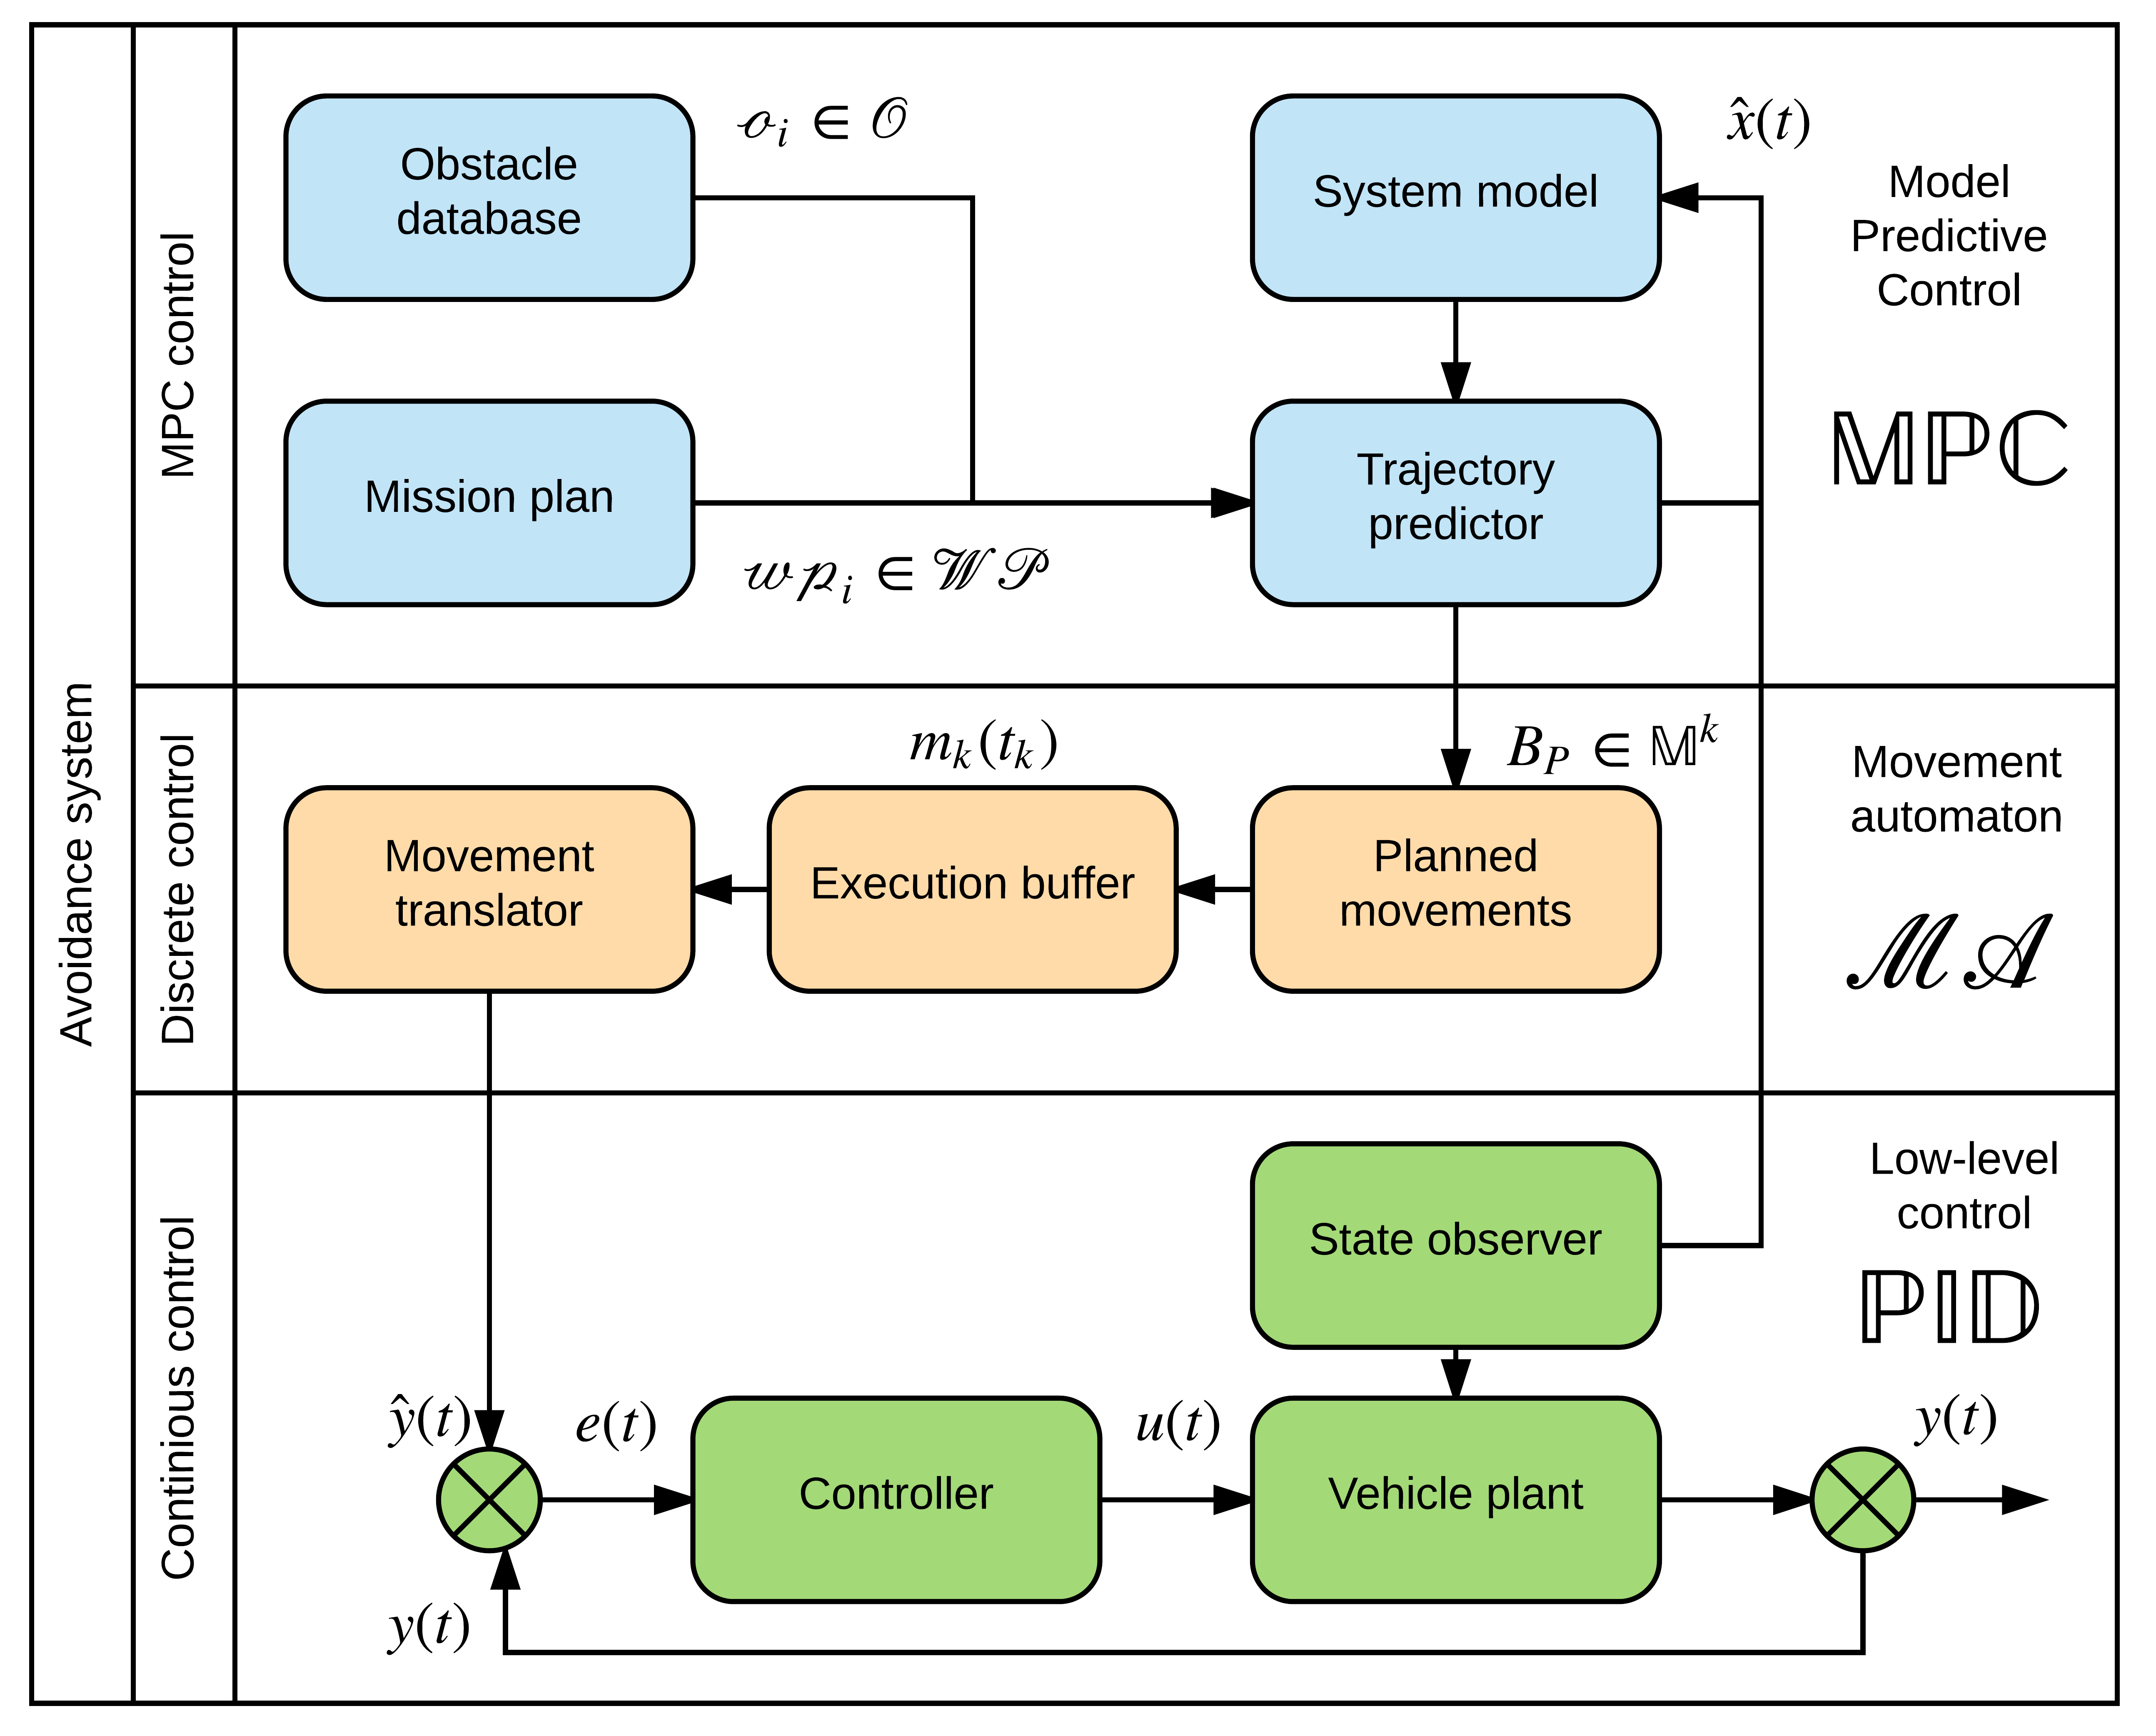
\includegraphics[width=.75\linewidth]{\FIGDIR/72_Control_Concept.png}
    \caption{Control concept for MPC with $\mathscr{MA}$.}
    \label{fig:controlConceptIntro}
\end{figure}

\noindent \textit{Event based control} module is responsible for abstract level decisions and mission execution. This module generates abstract level input commands which are optimal to given criterion. MPC in this case is taken into event base level. MPC in this work is triggered by consumption of of all movements in movement automaton $\mathscr{MA}$ buffer $B$. There is no re-planning trigger due to trajectory deviation from original estimation. The reason is that system model and Vehicle plant are using same model in simulation (in nonlinear form and in linearized form for predictor)  \textit{Event based control} consist from following components:
\begin{enumerate}
    \item \textit{Obstacle database} - provides relevant obstacle data for trajectory planning, contains obstacle set $\mathscr{O}$ with obstacle records $o_i$. This module is data provider. Sensor fusion is omitted in this work.
    \item \textit{Mission plan} - contains mission plan $\mathscr{WP}$, determines navigation goal waypoint $\mathscr{WP}_g$.
    \item \textit{Trajectory predictor} - produces movement chain $B_p\in \mathbb{M}$. This module represents Model predictive control. It is using \textit{System model} to predict future states in finite prediction window. This module predicts trajectory between each waypoint $w_i,w_{i+1}\in\mathscr{WP}$. Prediction is invoked at time of decision $t_d$. Predictor then uses \textit{System model} with initial state $\hat{x}(t_d)$ form \textit{State observer} module. Predictor calculates optimal trajectory to avoid obstacles in obstacle set $\mathscr{O}$ and reach waypoint $w_{i+1}$.
    \item \textit{System model} - interprets system dynamics response to movement chain $m_1(t_1),\dots,m_i,t_i$ with initial state $x(t_0)=\hat{x}(t_{d_{i-1}})$. This module is mainly used to predict feasible trajectories around known obstacles set $\mathscr{O}$. \textit{System model} have been implemented as linear state predictor, because of system dynamics. Computation light techniques should be preferred in case of other non-linearizable systems. 
\end{enumerate}

\noindent \textit{Discrete control} module is responsible for processing abstract level movement command chain $B_p \in \mathbb{M}^k$. It is implemented as special type of open hybrid automaton, movement automaton $\mathscr{MA}$. Movement automaton $\mathscr{MA}$ have following notable modules:
\begin{enumerate}
    \item \textit{Planned movements} - buffers planned movements from avoidance grid $B_P\in\mathbb{M}^k$, planed movements buffer can be extended by additional movements (normal situation) or filled with new movement chain(flush) in case of trajectory correction or avoidance. Planned movement is similar to FIFO stack.
    \item \textit{Execution buffer} - executes first command from \textit{planned movements}, based on previous movement $m_{k-1}(t_{(k-1)})$ and actual command $m_k(t_k)$ chain of movement primitives $\{p_1, \dots p_l\}$ is created. Chain of movement primitives $\{p_1, \dots p_l\}$ is forwarded to movement translator (mapping module).
    \item \textit{Movement translator} - maps chain of movement primitives or other movement representation to:
    \begin{enumerate}[a.]
        \item \textit{Desired input signal $\hat{u}(t)$,} - in case of \textit{open loop control}, in this case desired control signal is feed directly to \textit{controlled plant}.
        \item \textit{Desired output signal $\hat{y}(t),t\in<t_{(k-1)},t_k)$} - in case of \textit{closed loop control}, in this case desired output signal is feed to closed loop controller. If there is closed loop controller, there is possibility for low level optimisation of control.
    \end{enumerate}
\end{enumerate}

\noindent \textit{Continuous control} module is target for low level control optimisation techniques. It is expected that \textit{controlled plant} is observable at least at position and orientation state parameters. \textit{State observer} provides observed state within critical time frame. \textit{Continuous control} module is responsible for low level control of plant with following modules:
\begin{enumerate}
    \item \textit{Control} - standard closed loop control component, using error $e(t)$ as input and actuating unit signal $u(t)$ as output.
    \item \textit{Controlled plant} - controlled vehicle plant, can be subsurface marine vehicle or aerial vehicle
    \item \textit{State observer} - observing state of controlled plant $\hat{x}(t)$.
\end{enumerate}

\subsection*{Trajectory prediction technique}
\noindent \textit{Trajectory} is constrained by set of waypoints $\mathscr{WP}$ and set of obstacles $\mathscr{O}$. Obstacle set $\mathscr{O}$ is constant. \textit{Trajectory search} in static environment is problem which needs to address following concurrent requirements:
\begin{enumerate}
    \item \textit{Calculation time} - avoidance trajectory calculation time must be shortest possible to assure optimal \textit{prediction window}.
    \item \textit{Estimation precision} - avoidance trajectory estimation must be precise enough to guarantee safety of predicted trajectory. Predicted trajectory with some estimation error, should not lead to vehicle crash. 
    \item \textit{Estimation optimality} - predicted trajectory should minimize optimality criterion or cost function $J(\circ)$.
\end{enumerate}
\noindent In case of \textit{Estimation optimality} requirement, only known world is taken into account. For real \textit{Estimation optimality} all obstacles static or dynamic needs to be known at time of prediction. This constraint is not guaranteed in future obstacle avoidance system. This work consider all obstacles to be known prior the flight. This requirement can be reduced to \textit{Estimation sub-optimality}.

Model predictive control gives discrete time optimisation technique to be used used on obstacle avoidance \textit{event based control} level.  Continuous optimisation techniques to increase movement automaton $\mathscr{MA}$ execution precision can be used in \textit{closed loop control}. Chosen optimisation techniques for movement chain optimisation is \textit{rapid exploration tree}. This prediction technique is not trivial search technique and it demonstrates qualities of discrete time optimum search.

\subsection*{Type of sensory data and its processing}
\noindent In future solution \textit{LiDAR is main sensor}. There is planned addition for \textit{ADS-B} transceiver /receiver for moving cooperative obstacle Sense \& Avoid. LiDAR data will be represented as positional vector $\vec{p}=[d,\theta,\varphi]$, where $d$ is distance to point, $\theta$ is horizontal offset angle and $\varphi$ is vertical offset angle in local coordinates frame. Only one matter point $\vec{p}$ is scanned at given scanning time $t_s$, in case of LiDAR sensor with one active scanner. 

LiDAR data for one LiDAR sweep at time interval $(t_s, t_e] $are given as series of points and scanning time pairs $\left\{\{\vec{p}_1\,t_s\},\{\vec{p}_2,t_2\},\dots,\{\vec{p}_n,t_e\}\right\}$. These points needs to be normalized at time $t_e$ in \textit{local coordinate frame} with center at vehicle position $[x_v,y_v,z_v]$ and rotated by vehicle orientation $[-\alpha_v,-\beta_v,-\gamma_v]$. One LiDAR sweep covers area given by scanning distance $[d_s,d_e]$, horizontal range $[\theta_s,\theta_e]$ and vertical range $[\varphi_s,\varphi_e]$. One LiDAR sweep covers rectangular conical cut in front of the scanning vehicle. All mission $\mathscr{WP}$ area and obstacle set $\mathscr{O}$ is know prior the mission execution.

For global coordinates Earth geocentric reference model \textit{WGS-84} is used, therefore \textit{GPS} is considered as main source of position. In later stages mixed position mode using \textit{GLONASS} system can be incorporated. \textit{GLONASS} is using \textit{PG-90} reference model. Transformation between \textit{PG-90} and \textit{WGS-84} are mentioned in \cite{misra1996integrated}. For further mentions of \textit{global coordinate frame} reference frame \textit{WGS-84} is always used.

\textit{Obstacle map} is using global coordinate frame, where obstacles are represented by center of their mass $\vec{p}_c$ and protective range $r$. Obstacle body is then given by unit ball around $\mathscr{B}(\vec{p}_c,r)$.

\noindent\textit{Sensor fusion} is fusing following data sources in local coordinate frame of vehicle:
\begin{enumerate}
    \item \textit{LiDAR sensor sweep (planned)} - based on LiDAR sensor reading point-cloud in front of vehicle is filtered by Extended Kalman Filter \cite{blanc2005ekf}. Visibility space is then partitioned into \textit{free, obstacle} and \textit{uncertain} subspaces.
    \item \textit{Obstacle map (planned)} - based on known obstacle map, the obstacles in Field Of Vision range are selected and fused into vehicle`s local coordinate frame. Free space previously unoccupied by by obstacles is marked as \textit{map obstacle occupied}.
    \item \textit{Intruders (planned)} - based on ADS-B reading and LiDAR data processing moving cooperative and non-cooperative intruders are identified. Portions of free space occupied by intruders in expected reach time are then marked as \textit{intruder occupied}.
\end{enumerate}

\noindent Result of future \textit{sensor fusion} will be used as base for \textit{Trajectory predictor}.

\subsection*{Obstacle avoidance}
\noindent \textit{Obstacle avoidance} is continuous process which is triggered by waypoint change. When \textit{Control strategy switch} changes mode to another waypoint following steps are executed until the reaching next waypoint:
\begin{enumerate}
    \item \textit{Next movement selection} - main contributor is \textit{Obstacle database}. \textit{Trajectory predictor} calculates critical distance to relevant obstacles $o_i\in\hat{\mathscr{O}}(t_{i-1})$ in predicted state $\hat{x}(t_i)$ after application of movement $m_i(t_i)$. Estimated obstacle set $\hat{\mathscr{O}}(t_i)$ is calculated after predicted movement execution.
    \item \textit{Feasibility assessment} - predicted movement state $\hat{x}(t_i)$ is compared to estimated obstacle set $\hat{\mathscr{O}}(t_i)$. If there is no approaching danger, movement is added to planned movements $B_p$ and next movement for $t_i=t_{i+1}$ is executed. If there is approaching danger systems use backtracking approach to determine feasible movements. If more than one movement is re-planned, then movement chain is changed according to new estimated movement chain.
\end{enumerate}
\noindent This approach is similar to \textit{Dynamic programming} backtracking.

\noindent Avoidance trajectory $\mathscr{T}(\vec{x}_i,t_i)$ generated for state $\vec{x}_i$ at decision time $t_i$. Executed movement buffer is given by chained prediction frames $\mathscr{P}(w_p)$. frames as  $\mathscr{T}= \cup_{i=\{wp_1,\dots,wp_n\}} \mathscr{T}(\vec{\hat{x}}_{wp_i},t_{wp_i})$ is optimal in known world \cite{kochenderfer2008encounter}.

\subsection*{Low level control}
\noindent \textit{Low level control} must be decoupled in order to implement movement automaton $\mathscr{MA}$. Various decoupling methods tor under-steered systems (less inputs than controlled variables) can be used, for example \cite{das2009dynamic}.

\section{Assumptions}
\noindent
The following assumptions are considered in this work:
\begin{assumption}{There is relevant obstacle database and no other static obstacles exists during a mission execution}\label{ass:1}\end{assumption}
\noindent Point-cloud is main source of constraints and obstacles. Main constraint is terrain and charted obstacles. Vehicle has discovered world prior the flight.  

\begin{assumption}{There are no moving obstacles.}\label{ass:3}\end{assumption}
\noindent This condition will be later relaxed after full \textit{sensor fusion} implementation.

\begin{assumption}{Estimates of the state of the UAV are available.}\label{ass:4}\end{assumption}
\noindent This condition is can be interpreted in way, that \textit{State observer} module can observe vehicle position $[x_v,y_v,z_v]$ and orientation $[\alpha_v,\beta_v,\gamma_v]$ in real time. 

\begin{assumption}{The operational space does not contain 'traps' such as caves. 'Traps' arise because the field of view of the LiDAR does not include the whole space surrounding the UAV.}\label{ass:5}\end{assumption}
\noindent \textit{Convex traps} can not be addressed by this approach, due the insufficient rules in \textit{Rule engine} module. When \textit{convex trap} avoidance rules will be implemented into rule engine it will be possible to relax this assumption.

\begin{assumption}{There is a mission plan for the UAV consisting of waypoints.} \label{ass:6} \end{assumption}

\noindent Trajectory given by mission plan is not optimal, because it is just joint lines between waypoints. Dynamic of most system does not allow to follow this type of route, therefore route considering reach set of vehicle $\mathscr{R}$ needs to be calculated prior the mission execution or \textit{Trajectory predictor} is used as route planning tool. 
\chapter{State of art}\label{ch:stateofArt}
\noindent
Cooperative and non cooperative Sense and Avoid (SAA) systems are key enablers for Unmanned Aircraft (UAV) to routinely access non-segregated airspace \cite{spriesterbach2013unmanned}. Both cooperative and non-cooperative SAA systems are being developed to address this integration requirement.
\noindent
The SAA capability is defined as the automatic detection of possible conflicts by the UAV platform under consideration and performing avoidance maneuver tasks to prevent the identified collisions. An analysis of the available SAA candidate technologies and the associated sensors for both cooperative and non-cooperative SAA systems is presented in \cite{muraru2011critical}. Non-cooperative Collision Detection and Resolution (CD\&R) for UAV is considered as one of the major challenges that needs to be addressed \cite{lai2012see} for the insertion of UAVs in non-segregated air space. As a result, a number of non-cooperative sensors for the SAA system have been adopted. Light Detection and Ranging (LIDAR)is used for detecting, warning and avoiding obstacles for low-level flying \cite{sabatini2014lidar}.

An approach to the definition of encounter models and their applications to SAA strategies is presented in \cite{kochenderfer2008encounter} for both cooperative and non-cooperative scenarios.

Since 2014, there is a visible strong political support for developing rules on drones but regulations are not harmonized yet. The European Aviation Safety Agency (EASA) has been tasked to develop a regulatory framework for drone operations and proposals for the regulation of "low-risk" UAV operations. In achieving this, EASA is working closely with the Joint Authorities for Regulation of Unmanned Systes (JARUS) \cite{jarus2016regulations}.


\section{UAV motion model}
\noindent
This section strongly follows \cite{lee2011structure}.

\subsection{Continuous-time systems}\noindent
%This is very imprecise. A good notation is:
%1. u is the control function. It is a map from a time interval to \R^p, i.e., u:[0,T] \to %\R^p. Thus you could write u\in \C^p
%2. u(t) is the value (in \R^p) of the control function u. It is correct to write u(t)\in %\R^p

%You have to say what \C^p is. I guess that you mean the space of continuous functions. If this is the case, this specification is very unnatural since this space is too restrictive. Controls of interest usually have discontinuities.  More common is L^1 (space of integrable functions).

\noindent Consider a class of systems given by functions:
\begin{equation}
    \begin{split}
    S&: \vec{u}(t)  \to \vec{x}(\vec{x}_0,t) \\
    \vec{u}&(t): [0,T] \to \R^p \\
    \vec{u}&(t)\in \mathbb{R}^p , \vec{x}(t) \in \mathbb{R}^n \\
    \end{split}
\end{equation}
where $\vec{u}(t)$ and  $\vec{x}(\vec{x}_0,t)$ are a sets of continuous-time signals.
These are often called continuous-time systems because they operate on
continuous-time signals. Frequently, such systems can be defined by differential
equations that relate the input signal to the output signal.
A prototypical description of a controlled (there is a control input signal)
continuous-time system is:
\begin{equation}\label{eq:nonlinearsystem}
    \dot{x}(t) = f(t,x(t),u(t)), u(t) \in U(t)
\end{equation}
where $f:\mathbb{R}\times\mathbb{R}^n\times\mathbb{R}^p\to\mathbb{R}^n$
satisfies the conditions for existence
and uniqueness of the ordinary differential equation and $u$ is our control\cite{butcher1987numerical}.

\subsection{Discrete-time systems}
\noindent
\noindent Consider another class of systems given by functions
\begin{equation}
    \begin{split}
    S&: \vec{u}(k)  \to \vec{x}(k), \\
    k& \in \{0, t_s, 2.t_s, 3.t_s, \dots i.t_s\}, i \in \N^+\\
    \vec{u}&(k)\in \mathbb{R}^p , \vec{x}(k) \in \mathbb{R}^n\\
    \end{split}
\end{equation}
where $\vec{u}(k), \vec{x}(k)$ is a set of discrete-time signals. They can be represented by a function $f$ like $f:\{0, t_s, 2.t_s, 3.t_s, \dots i.t_s\} \to \R^n,  i \in \N^+$ where $t_s$ is sampling time and $i$ is discrete step \cite{shampine1997matlab}.

%MPC
\section{Model Predictive Control}
\noindent Model predictive control (MPC) or receding horizon control (RHC) is a form of control in which the current control action is obtained by solving on-line, at each sampling instant, a finite horizon open-loop optimal control problem, using the current state of the plant as the initial state; the optimization yields an optimal control sequence and the first control in this sequence is applied to the plant. Nearly every application imposes constraints; actuators are naturally limited in the force (or equivalent) they can apply, safety limits states such as temperature, pressure and velocity and efficiency often dictates steady-state operation close to the boundary of the set of permissible states. The prevalence of hard constraints is accompanied by a dearth of control methods for handling them, despite a continuous demand from industry that has had, in their absence, to resort often to adhoc methods. Model predictive control is one of few suitable methods, and this fact makes it an important tool for the control engineer, particularly in the process industries where plants being controlled are sufficiently slow to permit its implementation. Other examples where model predictive control may be advantageously employed include unconstrained nonlinear plants, for which on-line computation of a control law usually requires the plant dynamics to possess a special structure, and time-varying plants. 

Determining the feedback solution, on the other hand, requires solution of the Hamilton-Jacobi-Bellman differential or difference equation, a vastly more difficult task (except in those cases, such as $H_2$ and $H_\infty$.

The feedback solution provided by MPC schemes can be obtained essentially in two ways:
\begin{enumerate}
    \item \textit{Open loop control optimization} - via Maximum Principle or other techniques (e.g., approximation by linear programming).
    \item \textit{Closed loop control optimization} - via Dynamic Programming.
\end{enumerate}

\begin{figure}[H]
    \centering
    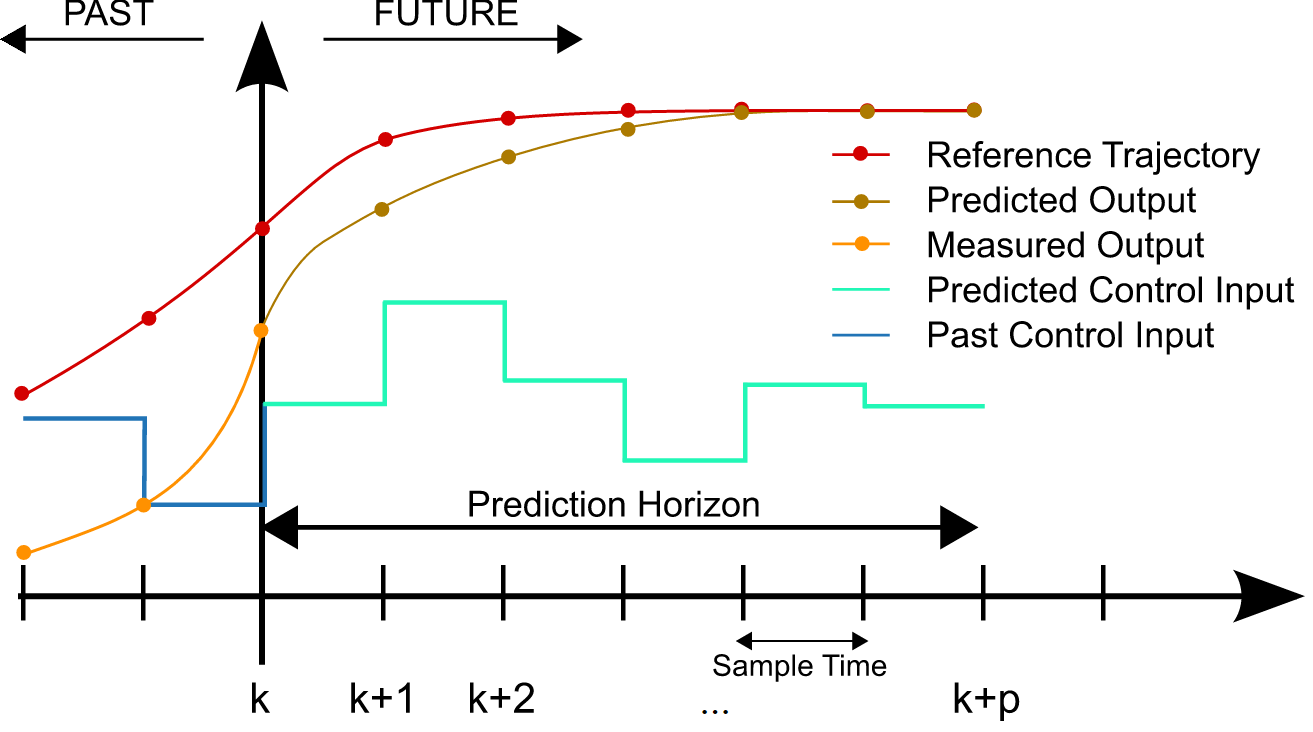
\includegraphics[width=.75\linewidth]{\FIGDIR/73_General_MPC_Scheme.png}
    \caption{General Model Predictive Control concept.}
    \label{fig:generalMPCConcept}
\end{figure}

\noindent General MPC concept is portrayed in figure \ref{fig:generalMPCConcept} for discrete time case. Usual notation is used for MPC:
\begin{enumerate}
    \item\textit{Reference trajectory} $\tilde{x}(i),i\in\left\{t_0,\dots,k,\dots,T\right\}$
    \item\textit{Predicted output} $\hat{x}(i),i\in\left\{k,\dots,T\right\}$
    \item\textit{Measured (real) output} $x(i),i\in\left\{t_0,\dots,k,\dots,T\right\}$
    \item\textit{Predicted control input} $\hat{u}(i),i\in\left\{k,\dots,T-1\right\}$
    \item\textit{Past control input} $u(i),i\in\left\{t_0,\dots,k-1\right\}$
\end{enumerate}

\noindent In general system is formulated as follow:
\begin{equation}
    \begin{aligned}
        x(k+1) &= f(x(k),u(k)), u(k)\in\mathbb{U}, x(k)\in\mathbb{X}\\
        y(k) &= h(x(k))\\
    \end{aligned}
\end{equation}
\noindent Where $f(\cdot)$ is defined by the originating differential equation that has an equilibrium point at the origin $f(\vec{0},\vec{0}) = \vec{0}$. Equation form $x^+=f(x,u)$, $y=h(x)$ is often used for shorter notation. Usually $\mathbb{U}$ is a convex compact subset of $\mathbb{R}^m$ and $\mathbb{X}$ is convex, closed subset of $\mathbb{R}^n$. For event $(x,k)$ the cost of steering is defined by function $V$:
\begin{equation}
    V(x,k,u)= \sum_{i=k}^{k+N+1}\mathpzc{l}(x(i),u(i)) + F(x(k+N))
\end{equation}
\noindent Where $u=\left\{u(k), u(k+1),\dots,u(k+N-1)\right\}$ and $x(i)= x^u(i;(x,k))$. One can assume that stage cost $\mathpzc{l}(x,u)\ge c(|(x,u)|)^2$, $\mathpzc{l}(0,0)=0$. The terminal time $k+N$ increases with time $k$ and is often referred as \textit{receding horizon}. A terminal constraint given by following equation:
\begin{equation}
    x(k+N) \in X_f \subset \mathbb{X}
\end{equation}
\noindent At event $(x,k)$ the optimal problem $\mathscr{P}(x,k)$ of minimizing cost functional $V(x,k,u)$, subject to the control, state and terminal constraint is solved yielding the optimizing control sequence:
\begin{equation}
    \hat{u}(x,k) = \left\{\hat{u}(k,(x,k)),\hat{u}(k+1,(x,k)),\dots,\hat{u}(k+N-1,(x,k))\right\}
\end{equation}
\noindent And the cost functional is equal to optimal cost:
\begin{equation}
    \hat{V}(x,k) = V(x,k,\hat{u}(x,k))
\end{equation}
\noindent The argument $(x,k)$ denotes initial state $x$ at time of prediction $k$. This defines an MPC law $\mathpzc{k}(x,k)=\hat{u}(k;(x,k))$. Since $\mathpzc{l}(\cdot)$ and $f(\cdot)$ are time invariant the problems $\mathpzc{P}(x,k)$ are invariant in the sense $\hat{V}(x,k)=\hat{V}(x,0)$ and $\mathpzc{k}(x,k)=\mathpzc{x,0}$ for all times $k$, so that is suffices, at each event $(x,k)$ to solve $\mathscr{P}_N(x,k)=\mathscr{P}(x,0)$. Problem of optimisation with finite horizon $N$ can be defined by:
\begin{equation}\label{eq:m19}
    \mathscr{P}_N(x):V_N^0(x)= \text{min}\left\{V_N(x,u)|u\in\mathscr{U}_n(x)\right\}
\end{equation}
\noindent Where $V_N(x,u)$ is given as follow:
\begin{equation}\label{eq:m110}
    V_N(x,u)= \sum_{i=0}^{N-1} \mathpzc{l}(x(i),u(i)) + F(x(N))
\end{equation}
\noindent Set of feasible control sequences $u=\left\{u(0),u(1),\dots,u(N-1)\right\}$, $x(i)=x^u(i;(x,0))$ and $\mathscr{U}_N(x)$ is the set of feasible control sequences satisfying the control, state and terminal constraints. Because the prediction horizon $N$ is finite, the minimum exists if $f(\cdot)$, $\mathbb{l}(\cdot)$ and $F(\cdot)$ are continious, $\mathbb{U}$ is compact, $X_f$ and $\mathbb{X}$ are closed. At event $(x,k)$ the problem $\mathscr{P}_N(x)$ is solved yielding the optimizing control sequence as follow:
\begin{equation}\label{eq:m111}
    \hat{u}(x)=\left\{\hat{u}(0,x),\hat{u}(1,x),\dots,\hat{u}(N-1,x)\right\}
\end{equation}
\noindent Optimal state trajectory is defined as follow:
\begin{equation}\label{eq:m112}
    \hat{x}(x)=\left\{\hat{x}(0,x),\hat{x}(1,x),\dots,\hat{x}(N,x)\right\}
\end{equation}
\noindent With value function defined as follow:
\begin{equation}\label{eq:m113}
    \hat{V}_N = V_N(x,\hat{u}(x))
\end{equation}
\noindent The single argument $\hat{x}$ denotes the initial state is $x$ at time $0$, so $\hat{x}(0,x)=x$. The first control $\hat{u}(0,x)$ is optimizing the sequence $\hat{u}(x)$ applied to the plant. The MPC law is is time invariant and is given as follow:
\begin{equation}\label{eq:m114}
    \mathpzc{k}_N(x)=\hat{u}(0,x)
\end{equation}
\noindent \textit{Dynamic programming} could in principle, be used to determine sequence $\{V_j(\cdot)\}$ of value function and a sequence of control laws $\{\mathpzc{k}_j(\cdot)\}$, where j is time to go. Because the optimal control problem is deterministic (in known environment), the value function $\hat{V}_N(\cdot)$ and its associated control law $\mathpzc{k}_N(\cdot)$ obtained via dynamic programming are \textit{identical} to the value function and control law in (\ref{eq:m113}) and (\ref{eq:m114}). It would be preferable to precompute $\mathpzc{k}_N(\cdot)$ using dynamic programming. Since this is usually impossible MPC computes at event $(x,k)$ the optimal control action $\mathpzc{k}_N(x)$ rather than pre-computing the control law $\mathpzc{k}_N(\cdot)$. The difference between MPC and Dynamic programming is in optimality guarantee. MPC with finite horizon $H_n$ gives optimal control law $\mathpzc{k}_n(\cdot)$ for given time-frame. In case that system run is longer than prediction window $n$. The control law is chained and therefore sub-optimal. Dynamic Programming guarantees optimality due it structure. Overall MPC can be seen as sequence a sequence of partial horizon optimization problems that approximates the optimization on the whole time horizon. MPC has obvious computational complexity advantages but, under favorable conditions, only guarantees a certain sub-optimality. Dynamic Programming guarantees optimality under certain conditions. Dynamic Programming usually has memory problem in long term runs.

One can find it convenient to refer to the infinite horizon value function $\hat{V}_\infty(\cdot)$ and the associated control law $\mathpzc{k}_\infty(\cdot)$ for the problem $\mathscr{P}_\infty(x)$ defined as (\ref{eq:m19}-\ref{eq:m111}), with finite horizon $N$ replaced by infinite horizon $\infty$, under assumptions that the minimum in (\ref{eq:m19}) exists.

\subsection{Stability and inverse optimality}
\noindent Model predictive control of constrained system is nonlinear necessitating the use of Lyapunov stability theory. Lyapunov stability was first proven by Chen and Shaw 1982 \cite{chen1982receding}. The value function of finite or infinite horizon can be used as Lyapunov function to establish stability of continuous time receding horizon control of unconstrained systems, when terminal equality constraint is employed. These results was extended by Mayne and Michalska \cite{mayne1990implementable} in 1990. Keerthi and Gilbert  \cite{keerthi1988optimal} first employed the value function as Lyapunov function for establishing stability of MPC of TB, constrained, non-linear discrete time systems. Therefore the value function is almost universally employed as  a natural Lyapunov function for stability analysis of model predictive control.

For any function $\Phi(x,u)$, let $\overset{\ast}{\Phi}(x,u)$ denote change in $\Phi(\cdot)$ as the state changes from $x$ to $x^+=f(x,u)$, for example $\overset{\ast}{\Phi}(x,u)=\Phi(f(x,u)-\Phi(x))$. Two distinct, but related, methods for establishing stability have evolved in the literature each yielding its own insights. Both approaches employ the value function $\hat{V}_N(\cdot)$ as a Lyapunov function. It is assumed, in the sequel that value function is continuous. The first approach, which is called \textit{direct method}, employs the value function and obtains conditions of $F(\cdot)$, $X_f$ and $\mathpzc{k}(\cdot)$ that ensures following inequality:
\begin{equation}\label{eq:m31}
    \overset{\ast}{\hat{V}}_N(x,\mathpzc{k}_N(x)) \le 0
\end{equation}
\noindent The second method uses the fact that following equality hold:
\begin{equation}
    \overset{\ast}{\hat{V}}_N(x,\mathpzc{k}(z) + \mathpzc{l}(x,\mathpzc{k}(x)))=\hat{V}_N(x^+)-\hat{V}_{N-1}(x^+)
\end{equation}
\noindent The right hand side of this equation is negative, either directly or by showing $\hat{V}_0(\cdot) \le \hat{V}_1(\cdot)$ implies $\hat{V}_{i-1}(\cdot) \le \hat{V}_i(\cdot)$, for all $i \ge 0$.

\subsection*{Direct method}
\noindent Main purpose here is to define from the expansive literature on model predictive control essential principles presented belows as axioms, that ensures closed-loop stability. This requires the determination of appropriate conditions of the ingredients $F(\cdot)$, $X_f$ and $\mathpzc{k}_f$. present in the most forms of the model predictive control. For each integer $k$, let $X_k$ denote  the set of states $x$ steerable by admissible control sequences to $X_f$ in $k$ steps or less. An admissible (or feasible) control sequence $u=\left\{u(0), u(1),\dots,u(k-1)\right\}$ satisfies the control state and terminal constraints: $u(i)\in\mathbb{U}$ for $i=0,1,\dots,k-1$, $x(i,x)\in\mathscr{X}$ for $i=0,1,\dots,k$ and $x(k,x)\in X_f$. The set of states that can be controlled by MPC with fixed horizon $N$ is $X_n$. Suppose then, that $x\in X_N$ and that the control sequence $u^0(x)$ that solves problem $\mathscr{P}_N(x)$ has been determined. Let $x^0(x)=\{x,x^0(1,x),\dots,x^0(N,x)\}$ denote the optimal state trajectory. The MPC $u=\mathpzc{k}(x)=u^0(0,x)$ steers the initial state $x$ to the successor state $x^+=x^0(1,x)=f(x,\mathpzc{k}_N(c))$. Goal is to determine a feasible control sequence $\tilde{u}(x)$ for $x^+$ to $x^0(N,x)\in X_f$. To obtain feasible control for $\mathscr{P}_N(x^+)$ one element $u$ is added to this sequence to obtain $\{u^0(1,x),\dots,u^0(N-1,x),u\}$, this sequence will be feasible for $\mathscr{P}_N(x^+)$ if $u\in\mathbb{U}$ and $u$ steers $x^0(N,x)\in X_f$ which in the case if $u=\mathpzc{k}_f(x^0(N,x))$ and $X_f$ and the local controller $\mathpzc{k}_f(\cdot)$ have following properties: $X_f \subset \mathbb{X}, \mathpzc{k}_f(x)\in\mathbb{U}$ and $f(x,\mathpzc{k}_f(x))\in X_f$, $\forall x \in X_f$ so that $X_f$ is positively invariant when the control law is $\mathpzc{k}_f(\cdot)$. If these conditions are satisfiedd the control sequence given by following equation:
\begin{equation}
    \tilde{u}(x) = \left\{u^0(1,x),\dots,u^0(N-1,x),\mathpzc{k}_f(x^0(N,x))\right\}
\end{equation}
\noindent Control sequence $\hat{u}(x)$ is feasible for $\mathscr{P}_N(x^+)$. The state trajectory resulting from initial state $x^+=x^0(1,x)$ and control sequence $\tilde{u}(x)$ is given by following equation:
\begin{equation}
    \tilde{x}(x)= \left\{x^0(1,x),\dots,x^0(N,x),f(x^0(N,x),\mathpzc{k}(x^0(N,x)))\right\}
\end{equation}
\noindent The associated cost is given by following equation:
\begin{equation}
    \begin{split}
        V_N(x^+,\tilde{u}(x)) = & V_N^0(x) - \mathpzc{l}(x,\mathpzc{k}_N(x))-F(x^0(N,x))\\
         +& \mathpzc{l}(x^0(N,x),\mathpzc{k}_f(x^0(N,x)))\\
         +& F(f(x^0(N,x),\mathpzc{k}_f(x^0(N,x))))
    \end{split}
\end{equation}
\noindent This cost which is an upper bound for $V_N^0(x^+)$ satisfies $V_N(x^+,\tilde{u}(x))\le V_N^0(x)-\mathpzc{l}(x,\mathpzc{k}_N(x))$ if $\overset{\ast}{F}(x,\mathpzc{k}_f(x))+\mathpzc{l}(x,\mathpzc{k}_f(x))\le 0$ if and only if $[\overset{\ast}{F}+\mathpzc{l}](x,\mathpzc{k}_f(x))\le 0$, $\forall x \in X_f$. Since the sum of the last three terms in the expression for $V_N(x^+\tilde{u}(x))$ is less than or equal to zero, this condition holds if $F(\cdot)$ is control Lyapunov function in the neighbourhood of the origin and $\mathpzc{k}(\cdot)$ and $X_f$ are chosen appropriately. If this condition holds, then (\ref{eq:m31}) also holds for all $x\in X_N$ which is sufficient to ensure thaht the state of closed loop system $x^+=f(x,\mathpzc{k}_N(x))$ converges to zero as $k\to\infty$ if its initial state lies in $X_N$. This motivates the following conditions that if satisfied ensure closed-loop  asymptotic stability if further minor assumptions are satisfied:

\begin{assumption}{$X_f \subset \mathbb{X}$, $X_f$ closed, $0\in X_f$ (state constraint satisfied in $X_f$)}\label{ass:m01}\end{assumption}
\begin{assumption}{$\mathpzc{k}_f(x)\in\mathbb{U}$, $\forall x \in X_f$ (control constraint satisfied in $X_f$)}\label{ass:m02}\end{assumption}
\begin{assumption}{$f(x,\mathpzc{k}(x))\in X_f$, $\forall x\in X_f$ ($X_f$ is positively invariant under $\mathpzc{k}_f(\cdot)$)}\label{ass:m03}\end{assumption}
\begin{assumption}{$[\overset{\ast}{F}+\mathpzc{l}](x,\mathpzc{k}_f(x)) \le 0$, $\forall x\in X_f$ ($F(\cdot)$ is local Lyapunov function)}\label{ass:m04}\end{assumption}

\noindent Assumption \ref{ass:m04}. implies assumption \ref{ass:m03}. if $X_f$ is a level set of $F(\cdot)$, this is a common situation. These conditions provide a concise characterization. The control sequence $\tilde{U}(x)$, in addition to providing and upper bound for $V_N^0(x)$, can also be usefully employed to initialize the algorithm for solving $\mathscr{P}_N(x^+)$. The conditions are of course merely sufficient.

\subsection*{Inverse optimality}
\noindent Bitmead et al. \cite{bitmead1990adaptive} show, in the context of linear unconstrained systems, that if the monotonicity property holds, the (finite horizon) value function $V_N^0(\cdot)$ is also the \textit{infinite horizon} value function of modified problem, an interesting example of inverse optimality. The known advantages of infinite horizon optimal control then accrue. Of course stability can be established independently as shown above. Inverse optimality can be easily extended to the nonlinear case as shown in \cite{magni1997stability}, for nonlinear unconstrained continuous time systems. The equation may be written in form:
\begin{equation}\label{eq:m33}
    V_N^0 (x) = \bar{\mathpzc{l}}(x,\mathpzc{k}_N(x))+ V_N^0(f(x,\mathpzc{k}_N(x)))
\end{equation}
\noindent For all $x\in X_N$ where $\bar{\mathpzc{l}}(x,u)=\mathpzc{l}(x,u)+[V_{N-1}^0-V_N^0](f(x,\mathpzc{k}_N(x)))$ and $\bar{\mathpzc{l}}(x,u)\ge\mathpzc{l}(x,u)\ge c|(x,u)|^2$. If assumptions \ref{ass:m01}.-\ref{ass:m04}. hold equation (\ref{eq:m33}) is fake Hamilton-Jacobi-Bellman algebraic equation corresponding to infinite horizon optimal control problem $\mathscr{P}_\infty(x)$ with $\mathpzc{l}(\cdot)$ replaced with $\bar{\mathpzc{l}}(\cdot)$. It is analogue to fake Riccati equation introduced in \cite{poubelle1988fake}. The controller $\mathpzc{k}_N(\cdot)$ is optimal for the modified problem, inherits known robustness properties of infinite horizon optimal control for nonlinear system satisfying dynamics $\dot{x}=f(x)+g(x)u$ as shown in \cite{magni1997stability}.

\subsection{Robustness}
\noindent The introduction of uncertainty in the system description raises the question of robustness, i.e. the maintenance of certain properties such as stability and performance in the presence of uncertainty. Most studies on robustness consider unconstrained systems; if a Lyapunov function for the nominal closed-loop system maintains its descent property if the disturbance (uncertainty) is sufficiently small, then stability is maintained in the presence of uncertainty. However, when constraints on states and controls are present, it is necessary to ensure, in addition, that disturbances do not cause transgression of the constraints; this adds an extra level of complexity. The earliest analyses of robustness of model predictive control employed impulse response models. Richalet study \cite{richalet1978model} investigate robustness in the face of gain mismatch. In later papers, control is determined by solving a min-max optimal control problem where the adversary represents uncertainty in the impulse response. The complexity of this problem increases exponentially with horizon length although Allwright \cite{allwright1993min} shows how this complexity may be substantially reduced. For further discussion of robustness of model predictive control using impulse response models, see \cite{zheng1993robust,genceli1993robust,de1996robustness}. It is relatively simple to ensure robust stability for linear or nonlinear systems that have finite memory finite impulse response models,finite Volterra models, etc.) since a stability constraint $x(N)=0$ is simply implementable, by choosing $N$ and $k_1$ aproppriately and imposing the constraint in the optimal control problem that the control is zero for all $k > k_1$.

There are several approaches to the study of robustness. The first is concerned with the robustness of closed-loop systems, designed using the nominal system (i.e. neglecting uncertainty). The second attempts to achieve robustness in the context of conventional model predictive control by consideration of all possible realizations on the uncertainty min-max open-loop model predictive control). A defect of model predictive control of uncertain systems, not yet widely appreciated, is the open-loop nature of the optimal control problem; the third approach addresses this by introducing feedback in the min-max optimal control problem solved on-line. 

\subsection*{Modeling uncertainty}
\noindent It should be supposed that uncertain system is  described by following equation:

\begin{equation}
    x^+ = f(x,u,w)
\end{equation}
\noindent The state $x$ and control $u$ satisfy the same constraints as before and the adversary $W$ satisfies $w(k)\in W(x(k),u(k))$ for all $k$ where, for each $(x,u)$, $W(x,u)$ is closed perhaps compact and constraints the origin in its interior. Because $f(\cdot)$ now depends on $w$ following equation is defined:
\begin{equation}
    \overset{\ast}{\Psi}(x,u,w)=\Psi(f(x,u,w))-\Psi(x)
\end{equation}
\noindent Where $\Psi(x)$ is any function. Let $w(\cdot)$ or $w=\{w(0), w(1),\dots, w(N-1)\}$ denote a disturbance sequence and $x^{u,w}(\cdot,x)$ the state trajectory resulting from an initial state $x$ at time 0, and control disturbance sequences $u$ and $w$ respectively. Let $\mathscr{F}(x,u)=f(x,u,W(x,u))$, then $\mathscr{F}(\cdot)$ maps points in $\mathbb{X}\times\mathbb{U}$ to subsets of $\mathbb{R}^n$ and $x^+\in\mathscr{F}(x,u)$ is an alternative definition of system. In some situations the uncertainty is time varying in which case uncertainty may be better modelled by $w(k)\in W_k$, where $W_k$ varies appropriately with some time $k$.

By inherent robustness is mean robustness of the closed-loop system using model predictive control obtained ignoring uncertainty. This has been investigated in \cite{de1996robustness} and \cite{magni1997stability}.

Subsequent versions of robust model predictive control that consider all realizations of the disturbance sequence $w$ in the optimal control problem require strengthened assumptions. The ingredients $F(\cdot)$, $X_f$ and $\mathpzc{k}_f(\cdot)$ are therefore assumed, to satisfy robust version of assumptions \ref{ass:m01}.-\ref{ass:m04} for stability new set of assumptions is assumed:
\begin{assumption}{$X_f\subset\mathbb{X}$, $X_f$ closed compact set, $0 \in X_f$.}\label{ass:m01a}\end{assumption}
\begin{assumption}{$\mathpzc{k}_f(x)\in\mathbb{U}$, $\forall x \in X_f$.}\label{ass:m02a}\end{assumption}
\begin{assumption} {$f(x,\mathpzc{k}_f(x),w)\in X_f$, $\forall x \in X_f $, $\forall w\in W(x,\mathpzc{k}_f(x))$}\label{ass:m03a}\end{assumption}
\begin{assumption}{$[\overset{\ast}{F}+\mathpzc{l}](x,\mathpzc{k}_f(x),w)\le 0$, $\forall x \in X_f$, $\forall w \in W(x,\mathpzc{k}_f(x),w)$. }\label{ass:m04a}\end{assumption}
\noindent There exists such a triple in $F(\cdot)$ is a robust control Lyapunov function in neighbourhood of the origin. These assumptions ensure $[\overset{\ast}{F}+\mathpzc{l}](x,\mathpzc{k}_f(x),w)\le 0$ for  all $x$ in an appropriate set and all $w\in W(x,\mathpzc{k}_N(x))$ and hence asymptotic stability.

\subsection*{Open-loop min-max model predictive control}
\noindent Deterministic model predictive control has the property that $X_N$ is positively invariant for the closed loops system $x^+=f(x,\mathpzc{k}_N(x))$. If $x\in X_N$, then $x^+ \in X_{N-1}\subset X_N$. This property is lost when uncertainty is present. To recover this property it is necessary to consider all possible realizations of $x^+ \in \mathscr{F}(x,u)$ in the optimal control problem and ensure each realization satisfies the state, control and terminal constraints \cite{michalska1993robust,chen1997game,de1999robustness}. The cost of an individual realization is defined by following equation:
\begin{equation}
    J(x,u,w) = \sum_{s=0}^{N-1} \mathpzc{l}(x(s),u(s)) + F(x(N))
\end{equation}
\noindent Where , now $x(s)=x^{u,w}(s,x,0)$ and the cost is given by following equation:
\begin{equation}
    V_N(x,u)= \text{max}\left\{J(x,u,w)|w \in \mathscr{W}_N(x,u)\right\}
\end{equation}
\noindent Where $\mathscr{W}_N(x,u)$ is the set of admissible disturbance sequences. Other choices are sometimes made for example $V(x,u)$ may be cost $J(x,u,\vec{0})$ of the nominal system, where $0$ is the zero sequence. An interesting variant, in the context of model predictive control of stable linear uncertain systems, is proposed in \cite{badgwell1997robust}; here the optimal control problem incorporates a robust stability constraint, namely that the control reduces the cost associated with each possible realization (assumed finite in number) of the linear system. This is stronger than merely a reduction in the maximum cost. In some cases ($H_\infty$ model predictive control), $\mathpzc{l}(\cdot)$ is a function of $(x,u,w)$. Let $\mathscr{U}_N^{o1}(x)$ now denote the set of admissible control sequences $u$ satisfying the state, control and terminal constraints for \textit{every} admissible  disturbance sequence $w$. when the initial state is $x$. Clearly $\mathscr{U}_N^{o1}(x)\subset\mathscr{U}_N(x)$. For all $i\ge 0$, let $X_i^{o1}$ denote the set of states $x$ such that $\mathscr{U}_N^{o1}\neq\{\}$, $X_i^{o1}\subset X_i$ is set of states that can be robustly steered to $X_f$ in $i$ steps or less by any admissible control sequence $u$. Then the optimal open-loop control problem is defined by following equation:
\begin{equation}
    \mathscr{P}_N^{o1}(x): V_N^0(x) = \text{min} \left\{V_N(x,u)|u\in \mathscr{U}_N^{o1}(x)\right\}
\end{equation}
\noindent The solution $u^0(0,x)$ of $\mathscr{P}_N^{o1}(x)$ yields the min-max MPC law given by following equation:
\begin{equation}
    \mathpzc{k}_N^{o1}=u^0(0,x)
\end{equation}
\noindent Corresponding $u^0(x)$ is a bundle of optimal state trajectories $\{X^0(x,w)\}$, one for each admissible $w$, where:
\begin{equation}
    X^0(x,w) = \left\{x^0(0,x,w),x^0(1,x,w),\dots,x^0(N-1,x,w)\right\}
\end{equation}
\noindent By the definition of $\mathscr{P}_N^{o1}$, $x^0(N,x,w)\in X_f$ for each admissible $w$. The ingredients $F(\cdot)$, $X_f$ and $\mathpzc{k}_f(\cdot)$ are assumed to satisfy assumptions \ref{ass:m01}., \ref{ass:m02}, \ref{ass:m03a}. and \ref{ass:m04a}. At this point a difficulty arises: suppose $x\in X_N^{o1}$ and optimal control sequence $\{u^0(0,x),u^0(1,x),\dots,u^0(N-1,x)\}$ steers every $x^+ \in \mathscr{P}(x,\mathpzc{k}(x))$ to $X_f$ in $N-1$ steps or less so that $x^+ \in X_{N-1}^{o1}$ The difficulty is obtaining a feasible control \textit{sequence}:
\begin{equation}
    \tilde{u}(x)=\left\{u^0(1,x),\dots,u^0(N-1,x),v\right\}
\end{equation}
\noindent For $\mathscr{P}_N(x^+)$, where $x^+$ is any state of $\mathscr{P}(x,\mathpzc{k}_N(x))$. The control action $v \in \mathbb{U}$ is required to satisfy $f(x^0(N,x,w),v\omega_N)\in X_f$ for every $w \in \mathscr{W}(x,u^0(x))$. Condition \ref{ass:m03a}. does not ensure the existence of a $v$ with this property. Without feasible sequence, an upper bound for $V_N^0(x^+)$ cannot be obtained. One way of avoiding this impasse is to replicate fixed horizon strategy by a variable horizon strategy  \cite{michalska1993robust} in which decision variable is  $(u,N)$. Suppose $u^0(x), N^0(x)$ solves the resultant variable optimal control problem $\mathscr{P}(x)$, where:
\begin{equation}
    u^0(x) = \left\{u^0(0,x), u^(1,x),\dots,u^0(N^0(x)-1,x)\right\}
\end{equation}
\noindent Then $(\bar{u}(x),N^0(x)-1)$, where:
\begin{equation}
    \bar{u}(x)=\left\{u^(1,x),\dots,u^0(N^0(x)-1,x)\right\}
\end{equation}
\noindent $\bar{u}(x)$ is a feasible solution for the optimal control problem $\mathscr{P}(x^+)$ at any $x^+ \in \mathscr{P}(x,\mathpzc{k}_N(x))$. With $V^0(\cdot)$. With $V^0(\cdot)$ denoting the resultant value function and $\mathpzc{k}^{o1}(\cdot)$ the resultant model predictive control law, where:
\begin{equation}
    [\overset{\ast}{V}^0+\mathpzc{l}](x,\mathpzc{k}^{o1}(x),w)\le 0
\end{equation}
\noindent Given monotonicity property holds for all $x \in X_N^{o1}-X_f$, all $w\in W(x,\mathpzc{k}^{o1}(x))$. Inside $X_f$, a local robustly stabilizing control law $\mathpzc{k}_f(\cdot)$. With further modest assumptions, robust asymptotic stability results with a domain of attraction $X_N^{o1}$.

\subsection{MPC for tracking}
\noindent The origin represents, with a suitable change of coordinates, any desired equilibrium state $x_r$, such that $x_r \in \mathbb{X}$, and $u_r\in\mathbb{U}$, where $u_r$ is the equilibrium control $x_r=f(x_r,u_r)$. When the system being controlled is linear, and constant input and output disturbance is present,Muske and Rawlings \cite{muske1993receding} utilize estimates of the disturbances to compute a $(x_r,u_r)$ such that the equilibrium output $x_r$ is as close as possible to the desired set-point $r$($x_r=r$ if this is possible without transgressing constraints). For further reading on tracking constant reference signals see \cite{jha2013position,lee1997stable,rawlings1994nonlinear,meadows1998feedback}. 

For tracking arbitrary reference signals (rather than those generated by a finite-dimensional exogenous system $w^+=s(w)$ variants of reference governors have been proposed. Reference governors, initially developed for control of constrained linear systems (see, for example \cite{gilbert1994nonlinear}) assume that a primal controller has been designed to stabilize the plant and provide nice tracking properties in the absence of constraints. The reference governor then modulates the $r(t)$ to obtain signal $g(t)$ with the following
properties:$g(t)$ never causes the plant to saturate and $g(t)\to r(t)$ as $t\to\infty$. Model predictive reference governors, proposed in \cite{bemporad1997nonlinear,bemporad1998fulfilling} utilize predictions over the interval reference signal $[t,t+T]$ ($t$ is currect time) to determine $g(t)$.

\subsection{Dynamic programming}\label{s:dynap}
\noindent This section adds theoretical supplements to discrete time optimisation and open possibilities of movement automaton $\mathscr{MA}$ chain optimisation. Discrete time $t_i$ is denoted as $i$, state vector $\vec{x}(t_i)$ is denoted as $x(i)$, input vector $\vec{u}(t_i)$ is denoted as $u(i)$.
\noindent Let consider problem formulation which neglects final conditions and state space constraints.
\begin{equation}\label{eq:p91}
    \begin{split}
        &\text{Maximize } \sum_{i=0}^{N-1} f_0(i,x(i),u(i)) + \Phi(x(N))\\
        &\text{Subject to: }\\
        &\textit{Dynamics: } x(i+1) = f(i,x(i),u(i)),\quad
        i = 0,1,\dots,N-1\\
        &\textit{Initial conditions: } x(0)= x_0\\
        &\textit{Control constraints: } u(i)\in\Omega_i,\quad i = 0,1,\dots
        , N-1
    \end{split}
\end{equation}
\noindent In (\ref{eq:p91}), the state $x(i)$ and the control $u(i)$ belong to arbitrary sets $X$ and $U$ respectively. $X$ and $U$ may be finite sets, or finite-dimensional vector spaces, or even infinite dimensional spaces. Initial state $x_0\in X$ is fixed. Control constraints $\Omega_i$ are fixed subsets of $U$. Finally cost function $f_0(i,\cdot,\cdot):X\times U \to \R$, $\Phi: X \to \R$, $f(i,\cdot,\cdot): X \times U \to X$ are fixed functions.


\newpage\noindent The main idea underlying \textit{dynamic programming} involves embedding the optimal control problem (\ref{eq:p91}), in which the system starts in state $x_0$ at time $0$, into a family of optimal control problems with the same dynamics, objective function, and control constraint as in (\ref{eq:p91}) but with different initial states and initial times. More precisely, for each $x \in X$ and $k$ between 0 and N - 1, consider the following
problem:
\begin{equation}\label{eq:p92}
    \begin{split}
        &\text{Maximize } \sum_{i=k}^{N-1} f_0(i,x(i),u(i)) + \Phi(x(N))\\
        &\text{Subject to: }\\
        &\textit{Dynamics: } x(i+1) =  f (i,x(i),u(i)), \quad i = k,k+1,\dots, N-1.\\
        &\textit{Initial conditions: } x(k)=x_k.\\
        &\textit{Control constraint: } u(i) \in \Omega,\quad i = k,k+1,\dots,N-1
    \end{split}
\end{equation}
\noindent Since the initial time $k$ and initial state $x$ are the only parameters in the problem above, index (\ref{eq:p92})$_{k,x}$ to distinguish between different problems.

\begin{lemma}\label{lem:p01}
Suppose $u^*(k),\dots,u^*(N-1)$ is an optimal control for (\ref{eq:p92})$_{k,x}$ and let $x^*(k) = x,x^*(k+1),\dots,x^*(N)$ be corresponding optimal trajectory $\mathscr{T}$. \\
Then for any $l,k \le l \le N-1$, control $u^*(l),\dots,u^*(N-1)$ is an optimal control for (\ref{eq:p92})$_{l,x^*(;)}$
\end{lemma}
\begin{dokaz}
Suppose that lemma \ref{lem:p01} is invalid. Then there exists control $\hat{u}(l),\hat{u}(l+1),\dots,\hat{u}(N-1)$ with corresponding trajectory $\mathscr{T} = x^*(l),\hat{x}(l+1),\dots,\hat{x}(N)$ such that:
\begin{equation}\label{eq:p93}
    \sum_{i=l}^{N-1} f_0(i,\hat{x}(i),\hat{u}(i)) + \Phi(\hat{x}(N)) > \sum_{i=l} f_0(i,x^*(i),u^x(i)) + \Phi(x^*(N))
\end{equation}
\noindent But then consider the control $\tilde{u}(k),\dots,\tilde{u}(N-1)$ given by:
\begin{equation}
    \tilde{u}(i)=
    \begin{cases}
        u^*(i), & i=k,\dots,l-1\\
        \hat{u}(i), & i=l,\dots,N-1
    \end{cases}
\end{equation}
\noindent The corresponding trajectory $\mathscr{T}$ starting at state $x$ and time $k$, is $\tilde{x}(k),\dots,\tilde{x}(N)$ is given by equation:
\begin{equation}
    \tilde{x}(i)=
    \begin{cases}
        x^*(i), & i=k,\dots,l\\
        \hat{x}(i), & i=l,\dots,N
    \end{cases}
\end{equation}
\noindent The value of the objective function corresponding to this control for the problem (\ref{eq:p92})$_{k,x}$ is given as:
\begin{equation}
    \begin{split}
        &\sum_{i=k}^{N-1} f_0(i,\tilde{x}(i),\tilde{u}(i))+ \Phi(\tilde{x}(N))\\
        & = \sum_{i=k}^{l-1} f_0(i,x^*(i),u^*(i)) + \sum_{i=l}^{N-1} f_0(i,\hat{x}(i),\hat{u}(i)) + \Phi(\hat{x}(N))\\
        & > \sum_{i=k}^{N-1} f_0(i,x^*(i),u^*(i)) + \Phi(x^*(N))
    \end{split}
\end{equation}
\noindent Equation (\ref{eq:p93}) shows that $u^*(k),\dots,u^*(N-1)$ can not be optimal for (\ref{eq:p92})$_{k,x}$, which contradicts the hypothesis. Therefore lemma is valid.
\end{dokaz}

\noindent From now on assume that an optimal solution for (\ref{eq:p92})$_{k,x}$ exists for all $0 \le k \le N-1$ and for all $x\in$. Let $V(k,x)$ be the maximum value of (9.2)$_{k,x}$. $V$ is \textit{maximum value function}.

\begin{theorem}\label{th:p01}
Define $V(N,\cdot)$ by $V(N,x)=\Phi(x)$. $V(k,x)$ satisfies backward recursion equation:
\begin{equation}\label{eq:p94}
    V(k,x) = \text{Max}\left\{f_0(k,x,u)+V(k_1,f(k,x,u))|u\in\Omega_k\right\}, 0 \le k \le N-1
\end{equation}
\end{theorem}
\begin{dokaz}
Let $x\in X$, let $u^*(k),\dots,u^*(N-1)$ be an optimal control for (\ref{eq:p92})$_{k,x}$, let $x^*(k)=x,\dots,x^*(N)$ be corresponding trajectory $\mathscr{T}^*$ and $x(k)= x,\dots,x(N)$ be another trajectory. Then following inequality holds:
\begin{equation}\label{eq:p95}
    \sum_{i=k}^{N-1} f_0(i,x^*(i),u^*(i)) + \Phi(x^*(N)) \ge \sum_{i=k}^{N-1} f_0(i, x(i), u(i)) + \Phi{x(N)}
\end{equation}
\noindent by lemma \ref{lem:p01} the left hand side of (\ref{eq:p95}) equals to:
\begin{equation}
    f_0(k,x,u^*(k)) + V(k+1,f(k,x^*,u^*(k)))
\end{equation}
\noindent On the other hand by the definition of $V$ following statement holds:
\begin{equation}
    \begin{split}
    &\sum_{i=k}^{N-1} f_0(i,x(o),u(i)) + \Phi(x(N)) =  f_0(k,x,u(k))\\
    +& \sum_{i=k+1}^{N} f_0(i,x(i),u(i)) \Phi(x(N)) \le f_0(k,x,u(k)) + V(k+1,f(k,x,u(k)))
    \end{split}
\end{equation}
\noindent With equality if and only if $u(k+1),\dots,u(N-1)$ is optimal for (\ref{eq:p92})$_{k+1,x(k+1)}$. Combining these two factors we get following inequality:
\begin{equation}
    \begin{split}
    &f_0(k,x,u^*(k)) + V(k+1,f(k,x,u^*(k)))\\
    \ge & f_0(k,x,u(k)) + V(k+1,f(k,x,u(k)))
    \end{split}
\end{equation}
\noindent for all $u(k)\in\Omega_k$ which is equivalent to equation (\ref{eq:p94}) form theorem.
\end{dokaz}

\begin{corollary}
Let  $u(k),\dots,u(N-1)$ be any control for problem (\ref{eq:p92})$_{k,x}$ and let $x(k) = x,\dots,x(N)$ be the corresponding trajectory. Then following equality holds tor all $k \le l \le N-1$  if and only if the control is optimal for (\ref{eq:p92})$_{k,x}$:
\begin{equation}
    V(l,x(l)) \le f_0(l,x(l),u(l)) + V(l+1,f(l,x(l),u(l))), \forall l, k \le l \le N-1
\end{equation}
\end{corollary}
\begin{corollary}
For $k=0,1,\dots,N-1$, let $\psi(k,\cdot): X\to \Omega_k$ be such that:
\begin{equation}
    \begin{split}
    & f_0(k,x,\psi(k,x))+ V(k+1,f(k,x,\psi(k,x)))\\
    =&\text{Max}\left\{f_0(k,x,u)+ V(k+1,f(k,x_u))|u\in\Omega_k\right\}
    \end{split}
\end{equation}
\noindent Then $\psi(k,\cdot), k = 0,\dots,N-1$ is an \textit{optimal feedback control}, therefore for any $k,x$ the control $u^*(k),\dots,u^*(N-1)$ defined by $u^*(l)=\psi(l,x^*,(l)), k \le l \le N-1$ is optimal for (\ref{eq:p92})$_{k,x}$: if following equation holds:
\begin{equation}\label{eq:pcol2}
    x^*(l+1)=f(l,x^*(l),\psi(l,x^*(l))), k \le l \le N-1, x^*(k)=x
\end{equation}
\end{corollary}
\noindent Theorem \ref{th:p01} and corollary (\ref{eq:pcol2}) are the main results of dynamic programming. The recursion equation (\ref{eq:p94}) allows to compute the value function and in evaluating the maximum in (\ref{eq:p94}) one can also obtain the optimum feedback control. Note that this feedback control $\psi$ is optimum for all initial conditions, However unless we can find a \textit{closed form} analytic solution to (\ref{eq:p94}), the dynamic programming formulation may necessitate a prohibitive amount of computation, since we would have to compute and store the values of $V$ and $\psi$ for all $k$ and $x$.

The most common application of \textit{Dynamic Programming} is application to problems in operation research where one can obtain “closed-form” analytic solutions to be recursion equation for the \textit{value function} \cite{re1962applied,wagner1969principles}. In the case of \textit{sequential decision-making under uncertainties}, where \textit{Sense\&Avoid} in full form belong, \textit{Dynamic Programming} is about the only available general method \cite{howard1960dynamic}. Larson \cite{larson1968state} has developed computational techniques which greatly increase the range of applicability of \textit{Dynamic Programming} where closed-form solutions are not available. These results can be reused in case of movement automaton $\mathscr{MA}$.
% REACH SETS
\section{Reach sets}

\subsection*{Definition}
\noindent
The reach set of a system described by a differential equation is the
set of all states that can be reached from an initial state within a given time
interval.
\noindent For general case consider the system described by equation (\ref{eq:nonlinearsystem}).

\begin{definition}[Reach set starting at a given point]\label{def:reachset01}
Suppose the initial position
and time $(\vec{x}_0, t_0)$ are given. The reach set $\mathscr{R}[\tau; t_0, \vec{x}_0]$ of system (\ref{eq:nonlinearsystem}) at time $\tau \ge t_0$, starting at position and time $(\vec{x}_0, t_0)$ is given by:
\begin{equation}
    \mathscr{R}[\tau, t_0, \vec{x}_0] = \bigcup \{\vec{x}(\tau):\vec{u}(s)\in U(s),s \in (t_0,\tau]\}
\end{equation}
\end{definition}
\noindent Reach set starting at given set can be used to determine reach set in case of hybrid system input control switch and it is defined as follow:
\begin{definition}[Reach set starting at a given set]
The reach set at time $\tau > t_0$ starting from set $X_0$ is defined as:
\begin{equation}
    \mathscr{R}[\tau, t_0, X_0] = \bigcup \{R[\tau, t_0, \vec{x}_0]:\vec{x}_0 \in X_0\}
\end{equation}
\end{definition}

\newpage\noindent Reach set for adversarial behavior can be used to calculate possible escape routes from pursuer and it is defined as follow:
\begin{definition}[Reach set under adversarial behavior]
Consider now the case of adversarial behavior, for system $\dot{x}=u,u\in \mathbb{B}$.
where $u(t)$ is our control and $v(t)$ is adversary control which is independent of $u(t)$, let $w(t)=u(t)- \arg_{v(t)\in V(t)}\sup_{{x} \in x(t)} v(t)$, which represents worst possible input change in given state and time, then reach set for system is represented as:
\begin{equation}
    \mathscr{R}[\tau; t_0, \vec{x}_0] = \bigcup \{\vec{x}(\tau):\vec{w}(s) \in W(s),s \in (t_0,\tau]\}
\end{equation}

\end{definition}

\noindent Reach set under constraints are usable to define state constrained systems in terms of dynamics and technical capabilities.
\begin{definition}[Reach set under state constraints]
Suppose the initial position
and time $(\vec{x}_0, t_0)$ and $x$ constraints are given $x(t) \in \mathbb{A} \subset \R^n, \dot{x}(t) \in \mathbb{B} \subset \R^n$. The reach set $\mathscr{R}[\tau, t_0, \vec{x}_0]$ of system (\ref{eq:nonlinearsystem}) at time $\tau \ge t_0$, starting at position and time $(\vec{x}_0, t_0)$ is given by:
\begin{equation}
    \mathscr{R}[\tau, t_0, \vec{x}_0] = \bigcup \{\vec{x}(\tau):\forall s\in (t_0,\tau], x(s) \in \mathbb{A}, \dot{x}(s) \in \mathbb{B}, \exists u(s) \in U(s)\}
\end{equation}
\end{definition}

\section{Occupied space}
\noindent Occupied pace representation is crucial in obstacle avoidance, this section introduces models and notations. Analytical geometry structures of sphere and ellipsoid are used to  determine closed occupied spaces.
\begin{definition}{Unit sphere (Unit ball) $\mathscr{B}(\vec{p},r)$} denotes occupied space in point $\vec{p} = [x_p,y_p,z_p]^T$ with radius $r$. Where point $\vec{b} = [x_b,y_b,z_b]$ belongs to sphere $\mathscr{B}(\vec{p},r)$ if and only if:
\begin{equation}
    (x_b-x_p)^2 + (y_b-y_p)^2 + (z_b-z_p)^2 \le r
\end{equation}    
\end{definition}
Definition of sphere $\mathscr{B}(\vec{p},r)$ is usually used to denote safety margin of vehicle $s_m$, where $s_m$ represents maximum radius to vehicle matter point from vehicle mass center. 
\begin{definition}{Spherical coating $\mathscr{C}(\vec{f}(\cdot),r)$} denotes occupied space of object which surface can be approximated by function $f(\cdot)$, with points of surface $\vec{p}=[x_p,y_p,z_p]^T\in\R^3$ and object inner points $\vec{i}=[x_i,y_i,i_p]^T\in \R^3$. Then spherical coating $\mathscr{C}(\vec{f}(\cdot),r)$ is defined as follows:
\begin{equation}
    \mathscr{C}(\vec{f}(\cdot),r) = \left\{\vec{b} \in \R^3: \vec{b}\in \bigcup_{\forall \vec{p} \in \vec{f}(\cdot)} \mathscr{B}(\vec{p},r), \nexists \vec{i}=\vec{b}  \right\}
\end{equation}
One can say that spherical coating is a closed,not compact set of points $\vec{b} = [x_b,y_b,z_b]$  where distance to closest surface point $\vec{p}$ is lesser or equal to coating radius $r$.    
\end{definition}
\noindent Calculation of spherical coating can be time consuming especially when surface function $\vec{f}(\cdot)$ is not smooth \cite{sommerville2016analytical}. Closest point problem has been formulated by Shamos \cite{shamos1975closest}.Closest point estimation with moving vehicle and with thick data flow can by solved by time optimal and deterministic approach, one of them have been presented by Bentley in \cite{bentley1980optimal}. Approach is based on closest point search in local planar coordinates which may be ideal for steam-line LiDAR data. 
Estimation of spherical coating is used in potential field avoidance methods. One most notable study was using spherical approximation based on obstacle center and mass distribution in space \cite{borenstein1991vector}. Potential field have their limitations in partially known environment, because it is hard to determine center of mass and mass distribution of obstacle from partial information \cite{koren1991potential}. Main source of object proportional estimation can be reused from camera based solutions like \cite{oberkampf1993iterative}. Other possible solution sources from fast clustering algorithms from Geographical Information Systems (GIS) for example \cite{zaiane2002clustering}.

\section{Movement automaton}
\noindent Movement automaton used as proxy between discrete command chain (movement chain) and control signal ($u(t)$). Movement automation is based on hybrid automaton.
\begin{definition} {Hybrid automaton $\mathscr{H}(Q,\R^n,f,\varphi,\rho)$} is well defined system representation consisting from following components.
\begin{equation}
    \begin{aligned}
        Q &\equiv \textnormal{set of discrete states}\\
        \R^n &\equiv \textnormal{continuous state-space} \\
        f: Q\times \R^n \to \R^n & \equiv \textnormal{vector field}\\
        \varphi:Q\times \R^n \to Q & \equiv \textit{discrete transition}\\
        \rho : Q\times \R^n \to \R^n & \equiv\textit{reset map}\\
    \end{aligned}
\end{equation}
Discrete state $q_i \in Q$ represents system current state and impacts system behavioural equation and state. Continuous state $[x(t),u(t)]\in \R^n$ represents  system state from physical viewpoint (values of state variables and inputs in continuous space $\R^n$). Vector field $f$ assign to each discrete state $q_i \in Q$ system behavioral function $\dot{x} = f(x,u)$. Discrete transition $\varphi$ defines conditions to transit between two different states. Reset map $\rho$ defines system state or input change on reset conditions.
\end{definition} 

\begin{definition}{Trajectory primitive $\hat{t}(x_0,t_0,t_1)$} is defined on given time interval $(t_0,t_1]$ for system $\dot{x} = f(x,u)$ with initial state $x_0$ at $t_0$ and final state $x_1$ at $t_1$ as follow:
\begin{equation}
    \hat{t}(x_0,t_1,t_1) = \left\{ x\in\R^n: x = \Phi(t_0,\tau,x_0), \tau \in (t_0,t_1] \right\}
\end{equation}
Trajectory primitive can be viewed as ordered set of system trajectory positions, this set is infinite continuous and flat.    
\end{definition}

\begin{definition}{Trajectory equivalence.}
Let $\mathscr{T}$ be trajectory defined as ordered sequence of countable trajectory primitives:
\begin{equation}
    \mathscr{T} = \left\{ \bigcup_{i=0}^n \hat{t}_i(x_i,t_i,t_{i+1}) \right\}
\end{equation}
Trajectory $\mathscr{T}$ is time independent and contains at leas one trajectory primitive. Trajectory $\mathscr{T}_\alpha$ consist from $m\ge 1$ trajectory primitives and its smooth and continuous. Trajectory $\mathscr{T}_\beta$ consist from $n \ne m$ primitives and its smooth and continuous.  Trajectories $\mathscr{T}_\alpha \equiv \mathscr{T}_\beta$ if and only if:
\begin{equation}
    \forall x_i \in \mathscr{T}_\alpha \exists y_i \in \mathscr{T}_\beta: x_{i+1} \equiv y_{i+1}, i \in {0\dots k}
\end{equation}
Where $x_i$ and $y_i$ is i-th point of trajectorries in state space $\R^n$.
\end{definition}

\noindent Trajectory primitives and trajectory equivalence have been defined, therefore movement primitives and movement can be defined.

\begin{definition}{Movement primitive $p$} 
for system $\dot{x} = f(x,u)$ and time interval $(t_i,t_{i+1}]$ there is defined continuous input signal $u(t)$.
\begin{equation}
    p_i = u(t), t\in (t_i,t_{i+1}]
\end{equation}
\end{definition}

\noindent Movement primitives can be chained to give smooth input signal. if there is movement primitive $p_1$ and movement primitive $p_2$ they can be chained on time $\tau$ when $u_1(\tau) = u_2(\tau)$, therefore system state can be also chained $x_1(\tau) = x_2(\tau)$.
\begin{definition}{Movement m(t)} is defined as chain of movement primitives $\{p_1,p_2,\dots,p_n\}$. Movement is smooth function with existing derivation. 
\end{definition}
\noindent Movement is main building block of movement automaton, movement is defined by movement type and its duration, movement switching is possible when execution time allows movement chaining. Movements can be separated into two categories:
\begin{enumerate}
    \item \textit{Stationary movement} - movement signal is constant during time of movement execution
    \item \textit{Dynamic movement} - movement signal is evolving during time of movement execution.
\end{enumerate}
\begin{definition} {Movement automaton $\mathscr{MA}$}\label{def:movementAutomaton} for system defined by dynamics $\dot{x} = f(x,u)$ is a structure defined as follow:
\begin{equation}
    \begin{aligned}
    M&\equiv\textnormal{set of movements}\\
    u:M\times\R\to\R^m&\equiv\textnormal{input function evolution}\\
    \varphi:M\times M \times \R&\equiv\textnormal{movement transition map}\\
    B=M\times\R^2&\equiv\textnormal{movement buffer}\\
    \end{aligned}
\end{equation}
Movement $m_i\in M$ can be stationary or dynamic. Each movement in movement buffer has assigned duration $(t_i,t_{i+1}]\in\R^2$. Input function evolution $u(B,t)$ defines input evolution in given execution time $t = \tau+t_0, \tau\in(t_0,t_1]$.
Each movement $m_i$ in movement automaton $\mathscr{MA}$  is compliant with following rules:
\begin{enumerate}
    \item Each movement $m_i(t_{i},t_{i+1})$ has non zero duration.
    \item At switching time $\tau$ between movements $m_i$ and $m_{i+1}$, input function $u_i(\tau + t_i) = u_{i+1}(0)$.
    \item Each dynamic movement should be linking two static movement and vice-versa.
\end{enumerate}
\end{definition}

\newpage\subsection{Prediction stability of Movement Automaton}\label{s:maConvergence}
\noindent Because Movement automaton $\mathscr{MA}$ is abstract level control realized trough \textit{open loop hybrid automaton}, infinite receding horizon is questionable. This fact impacts the prediction reliability. This subsection formulates \textit{prediction horizon of movement automaton}.

\begin{definition}{Movement automaton $\mathscr{MA}$ prediction stability}\label{def:maPredictionStability}
For system $\dot{x}=f(x,\mathscr{MA})$ and predictor $\dot{\hat{x}}=f(\hat{x},\mathscr{MA})$ with separable nonlinear state $h(\cdot)$ and input transformation $g(\cdot)$ functions. With initial condition $x(t_0)=\hat{x}(t_0)=x_0$ and finite execution time $t\in[t_0,t_1]$. Prediction deviation $x(t)-hat(x)(t)$ stays in unit ball defined by:
\begin{equation}
    \mathscr{B}(x(t)-\hat{x}(t))= \left\{y\in\R^n:y=x(t)-\hat{x}(t),\norm{y}\le\rho\right\}
\end{equation}
\end{definition}

\begin{dokaz}
Let $\dot{x}=f(x,\mathscr{MA})$ be continuous time system, with state $x\R^n$ and control with movement automaton $\mathscr{MA}$. Input function $u(t)$ for movement buffer $B=\{m_1(t_1),\dots,m_i(t_i)\}$ is interpreted as chained input function:
\begin{equation}\label{eq:maTranslation}
    u(t)=
    \begin{cases}
        u(m_0,m_1,t_0,t_1)&:\textnormal{for } m_1(t_1)\\
        \vdots&\\
        u(m_{i-1},m_{i},t_{i-1},t_{i})&:\textnormal{for } m_i(t_i)
    \end{cases}
\end{equation}
\noindent Input function $u(t)$ (\ref{eq:maTranslation}) is smooth and differentiable as given by movement automaton $\mathscr{MA}$  definition (def. \ref{def:movementAutomaton}.). Let $w(t)$ be state noise function with boundary $\xi_w\in\R-\{\infty\}$, $v(t)$ input noise function with boundary $\xi_v\in\R-\{\infty\}$ and $\hat{x}(t)$ predicted state for movement chain $B=\{m_1(t_1),\dots,m_i(t_i)\}$. We can define function $V(t)$ as follow:
\begin{equation}
    V(t) = \frac{1}{2} (x(t)-\hat(x){t})^T\text{I}(x(t)-\hat(x)(t)) = (x(t)-\hat{x}(t))^2
\end{equation}
\noindent Given function can be derived by time $t$: 
\begin{equation}
    \dot{V}(t) = x(t)-\hat(x)(t)
\end{equation}
\noindent Controlled system with state $w(t)$ and input noise $v(t)$, where input and state are separable:
\begin{equation}
    \dot{x}=f(x,\mathscr{MA}) = g(x(t)+ w(t)) + h(u(t)+ v(t))
\end{equation}
\noindent Predicted system equation:
\begin{equation}
    \dot{\hat{x}}=f(\hat{x},\mathscr{MA}) = g(\hat{x}(t)) + h(u(t))    
\end{equation}
\noindent Therefore $\dot{V}$ is equal to:
\begin{equation}
    \begin{split}  
    \dot{V}(t) &= (g(x(t)+ w(t)) + h(u(t)+ v(t))) - (g(\hat{x}(t)) + h(u(t)))\\
               &=  g(w(t)) + h(v(t))
    \end{split}
\end{equation}
\noindent Member $g(x(t)-\hat{x}(t))$ is equal to zero, because of the premise that predicted $\hat{x}$ and real state $x$ are equal without state $w(t)$ and input noise $v(t)$ noise. Let us bound $g(w(t))$, boundary is straightforward in this case, because state noise $w(t)$ is bounded by $\xi_w$. Boundary is given as:
\begin{equation}
    \norm{g(w(t))} \le \norm{g(_{sup}(w(t)))} \le \norm{g(\xi_w)} \le \rho_w,\quad \rho_w\in\R^+-\{\infty\}
\end{equation}
\noindent Bounding member $h(v(t))$ will be problematic due to mapping function (\ref{eq:maTranslation}). Introducing input noise to movement automaton mapping function will cause input noise to be characterized like this:
\begin{equation}
    u(t)-\hat{u}(t)=\left(
    \begin{cases}
        u(m_0,m_1,t_0,t_1)+v_1(t)&\\
        \vdots&\\
        u(m_{i-1},m_{i},t_{i-1},t_{i})+v_i(t)^i&
    \end{cases}
    \right) -\left(
    \begin{cases}
        \hat{u}(m_0,m_1,t_0,t_1)&\\
        \vdots&\\
        \hat{u}(m_{i-1},m_{i},t_{i-1},t_{i})&
    \end{cases}
    \right) 
\end{equation}
\noindent This can be simplified to:
\begin{equation}
    \sum_{l=0}^{i} v_l(t)^l, \quad i\in\R^{+}-\{0,\infty\}
\end{equation}
\noindent So for case of input noise $v(t)$ member $h(v(t))$ of $\dot{V}(t)$ can be bounded like follow:
\begin{equation}
    \norm{h(v(t))} \le \norm{h(_{sup}\sum_{l=0}^{i} v_l(t)^l)}\le \norm{h(\xi^i)} \le \rho_v \quad \rho_v\in\R^+-\{\infty\}
\end{equation}
\noindent Where $i$ is finite count of movements in movement automaton $\mathscr{MA}$ buffer $B$, $i=|B|$. This parameter is cumulative which is given by member $\norm{h(_{sup}\sum_{l=0}^{i} v_l(t)^l)}$, but it is bounded by $\norm{h(\xi^i)}$. One can define boundary as follow:
\begin{equation}
    \norm{\dot{V}(t)} \le \rho_w + \rho_v = \rho, \quad \rho\in\R^+-\{\infty\}
\end{equation}
\noindent With boundary defined for derivation of $V(t)$ one can define boundary for $V(t)$ like follow for time of prediction $t_0$ and time of movement buffer execution end $t_i$:
\begin{equation}
    \norm{V(t)} \le \int_{t_0}^{t_i} \norm{\dot{V}(t)}\quad \text{d}t \le \int_{t_0}^{t_i} \rho \quad\text{d}t = \rho(t_i-t_0)
\end{equation}
\end{dokaz}
\subsection{Lyapunov stability of Movement Automaton}\label{s:maLyapunov}
\noindent It has been proven that system with movement automaton is stable in terms of finite receding horizon prediction. There is still open issue of \textit{Lyapunov stability}. To prove Lyapunov stability one needs to construct tracking problem of waypoint. Let say that system initial state $x(t_0)\in \mathscr{B}_s \subset \R^n$ is unit ball where system $\dot{x} = g(x) + h(u)$ is trying to reach equilibrium point $\hat{x}(t_i)$. Equilibrium point is predicted state $\hat{x}$ at final time of movement automaton $\mathscr{MA}$ buffer execution $t_i$. Then region of attraction $\mathscr{B}(\hat{x}(t_i),\rho)$, where $\hat{x}(t_i)$ is center of unit ball and $\rho$ is prediction deviation boundary at time $t_i$ given by definition (def. \ref{def:maPredictionStability}). Let us define system $y$ for tracking problem with equilibrium point $x(t_i)$ and initial state $x(t_0)\in\mathscr{B}_s$ for finite time period $t_\in[t_0,t_i]$
\begin{equation}
    y = {x}(t)-\hat{x}(t_i), \quad x(t_0)\in\mathscr{B}_s\subset\R^n, 
\end{equation}
\noindent It is obvious that region of attraction $\mathscr{B}(\hat{x}(t_i),\rho)$, is subset of $\mathscr{B}_s$. Let us define simple Lyapunov function $V(y)$ like follow:
\begin{equation}
    V(y) = \frac{1}{2}y^Ty = \frac{1}{2}\sum_{l=1}^n\left(x_l(t)^2-\hat{x}_l(t_i)^2\right)
\end{equation}
\noindent With derivation in time given by equation:
\begin{equation}
    \dot{V}(y)= \sum_{l=1}^n \frac{\partial V(y)}{\partial y_l}
\end{equation}
\noindent Now lets check second Lyapunov method stability conditions for $y$:
\begin{enumerate}
    \item $V(0)=0$ - this condition is valid, because Lyapunov function is 0 at equilibrium point $\hat{x}(t_i)$.
    \item $V(y) < 0, \forall y\in\mathscr{B}_s-\{0\}$ - this condition is valid, because $\frac{1}{2}\norm{y}>0,\forall y\in\mathscr{B}_s-\{0\}$.
    \item $\dot{V}(y)<0$ or $\dot{V}(y)\le0$ - convergence criterion is fully satisfied in case of no existing obstacle, because avoidance framework converges to goal waypoint exponentially fast.
\end{enumerate}
\noindent Convergence condition $\dot{V}(y)<0$ is not guaranteed in term of obstacle avoidance, because in some cases $\dot{V}(y)>0$ while avoiding enormous obstacle. Movement automaton $\mathscr{MA}$ is exponentially or at least asymptotic stable in terms of Lyapunov stability, within region of attraction $\mathscr{B}(\hat{x}(t_i),\rho)$. Obstacle avoidance framework is can be or can not be Lyapunov stable depending on obstacle set $\mathscr{O}$. Reachibility of waypoint $\hat{x}(t_i)$ is determined by system reachibility set $\mathscr{R}$.

\section{LiDAR}
\noindent LiDAR (Light Detection And Ranging) is active form of remote sensing: information is obtained from a signal which is sent from a transmitter and reflected by a target, and detected by a receiver back at the source. Following types of information can be obtained:
\begin{enumerate}
\item \textit{Range to target} - topographic LiDAR or laser altimeter.
\item \textit{Chemical properties of target} - differential absorption LiDAR.
\item \textit{Velocity of target} - Doppler LiDAR.
\end{enumerate}

\noindent Chemical properties of target are out of scope. Velocity of  target seems as interesting property to investigate, but this type of LiDAR is usually used for meteorological measurements of wind currents \cite{martin2011meteorological}. Extended research in LiDAR as obstacle detection sensor has been executed by research group around Sabatini \cite{sabatini2014lidar} and Ramasy \cite{ramasamy2016lidar}. 

LiDAR output is represented as point cloud it is described by following definition.
\newpage\begin{definition}[Scanned point and Point-cloud]
Consider viewpoint $v$ as origin of $\R^3$ space in 
Let point $p \in P$ be defined in polar coordinates:
\begin{equation}
    p= [ d, \theta, \varphi, t ]^T
\end{equation}
Where $d$ is distance to scanner, $\theta$ is horizontal angle from origin, $\varphi$ is vertical angle to origin, $t$ is time of retrieval.\\

\noindent Point-cloud is set of points scanned in small enough time-frame, based on processing raw point data it can have following representations:
\begin{enumerate}
\item Local point-cloud - position of sensor is used as origin of space and points can be represented in orthogonal or planar representation. 
\item Global point-cloud -global position of sensor is used as reference to calculate global position of points.
\end{enumerate}
\end{definition}

Point-cloud is usually addressed as \textit{raw point-cloud} in case if its represented in Local planar coordinates. Other forms of point cloud require further processing and they are not feasible for real time obstacle detection and avoidance \cite{chen2007airborne}.

\begin{figure}[H]
    \begin{subfigure}{0.5\textwidth}
    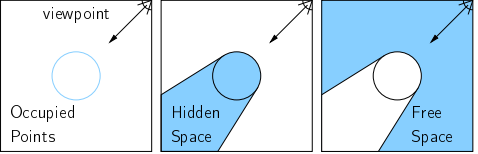
\includegraphics[width=0.9\linewidth]{\FIGDIR/10_Lidar_sets1.PNG} 
    \caption{Space type definitions}
    \label{fig:Spacetypes}
    \end{subfigure}
    \begin{subfigure}{0.5\textwidth}
    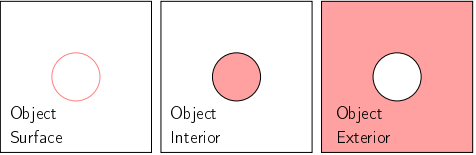
\includegraphics[width=0.9\linewidth]{\FIGDIR/11_Lidar_sets2.PNG}
    \caption{Object properties definitions}
    \label{fig:ObectProperties}
    \end{subfigure}
    \caption{Six spaces of interest \cite{yapo2008probabilistic}}
    \label{fig:Spaces of interests}
 \end{figure}
 
\noindent  Because of real-time obstacle avoidance it is necessary to introduce following terminology:
 \begin{enumerate}
 \item \textit{Occupied points} - points which have been detected by LiDAR (also addressed as visible points).
 \item \textit{Hidden space} - space which is hidden behind occupied points, from viewpoint it is uncertain what is in that space. 
 \item \textit{Free space} - space which is visible from viewpoint and it is not occupied by known objects.
 \item \textit{Object surface} - detected and undetected object surface
 \item \textit{Object interior} - occupied space by object.
 \item \textit{Object exterior} - free space around known objects.
 \end{enumerate}
 Existing method for space segregation \cite{yapo2008probabilistic} can yeld to following definition.
 \begin{definition}[Accessible space]\label{def:accessibleSpace}
    Consider known space $S$ as space explored by sensor (it can have different viewpoint along previous 3D trajectory).
    Intersection between \textit{object exterior} $S_E$ and \textit{free space}$S_F$ gives us \textit{Accessible space}.
    \begin{equation}
        S_A = S_E \cap S_F
    \end{equation}
 \end{definition}
 
 \noindent Accessible space $S_A$ (\ref{def:accessibleSpace}) is our bordering limitation for reachable space of system $R(\tau,t_0,\vec{x_0})$ (def. \ref{def:reachset01}.); 
\chapter {Detailed problem formulation}\label{ch:problemFormulation3D}
\noindent
Given a full known world, a mission plan, and a small UAV derive a safe approach to real-time route planning with a small computational footprint compatible with the low computational power available in small UAVs. The main application consists of terrain avoidance for low altitude flights. Following assumption holds:
\begin{enumerate}
  \item There is a obstacle database charting all obstacles prior the flight (\ref{ass:1}).
  \item There is an a-priory global terrain map, which does not change with time (\ref{ass:1}).
  \item There are no moving obstacles (\ref{ass:3}).
  \item Estimates of the state of the UAV are available (\ref{ass:4}).
  \item The operational space does not contain 'traps' such as caves. 'Traps' arise because the field of view of the LiDAR does not include the whole space surrounding the UAV (\ref{ass:5}).
  \item There is a mission plan for the UAV consisting of waypoints which are reachable with vehicle dynamics (\ref{ass:6}).
\end{enumerate}
\noindent
Following issues need to be addressed in practical implementation:
\begin{enumerate}
    \item \textit{Finite time mission execution} - approach must ensure that mission will be executed in finite time.
    \item \textit{Optimal route} - predicted route is optimal to given cost function and do not deviate from original mission plan.
    \item \textit{Solution respects vehicle dynamics} - estimated state $\hat{x}$ stays in reachable set of vehicle for prediction time frame $[t_0,t_i]$ and initial state $\hat{x}(t_0)$ is within reachable set $\mathscr{R}(\hat{x}(t_0):t_0,t_i)$
\end{enumerate}
\noindent
The integration of the proposed trajectory control of a UAV flight control framework is described next with reference to Figure \ref{fig:controlConceptIntro}, similar to $\mathscr{FOV}_{2D}$.

\section{Simple plane model}\label{sec:3DsimplisticplaneModel}
\noindent For avoidance theorem formulation in three dimensional space simplified rigid body kinematic model will be used. This model have decoupled roll, yaw and pitch angles which enables to provide simpler and more clean control (e.g movements can be simplified). 

\begin{equation}\label{eq:simple3dStatevector}
    \vec{x} = \left [ x_v,y_v,z_v,\alpha_v,\beta_v,\gamma_v \right ]^T
\end{equation}
State vector (\ref{eq:simple3dStatevector}) defined as positional state in euclidean position in right-hand euclidean space, where $x_v, y_v,z_v$ states, for latitude, longitude and altitude. Orientation angles for vehicle are $\alpha\beta,\gamma$ for roll, pitch, yaw angle.
\begin{equation}\label{eq:simple3dInputVector}
    \vec{u} = \left [ v, \omega_{\alpha_v}, \omega_{\beta_v},\omega_{\gamma_v}\right ]^T
\end{equation}
Input vector (\ref{eq:simple3dInputVector}) is defined as frontal velocity of vehicle $v$,orientation change in main axes as angular speed $\omega_{\alpha_v},\omega_{\beta_v},\omega_{\gamma_v}$
\begin{equation}\label{eq:simple3dvelocityDistribution}
    \begin{bmatrix}
    v_x\\
    v_y\\
    v_z\
    \end{bmatrix}
    = R_{XYZ}(\alpha_v,\beta_v,\gamma_v)
    \begin{bmatrix}
    v\\
    0\\
    0
    \end{bmatrix}
    =
    \begin{bmatrix}
        f_{v_x}(v,\alpha_v,\beta_v,\gamma_v)\\
        f_{v_y}(v,\alpha_v,\beta_v,\gamma_v)\\
        f_{v_z}(v,\alpha_v,\beta_v,\gamma_v)\\
    \end{bmatrix}
    =
    \begin{bmatrix}
         v\cos(\beta_v)\cos(\gamma_v)\\
         v\cos(\beta_v)\sin(\gamma_v)\\
         -v\sin(\beta_v)\\
    \end{bmatrix}
\end{equation}
Velocity distribution function (\ref{eq:simple3dvelocityDistribution}) is is defined trough standard rotation matrix (\ref{eq:xyzspaceRotationMatrix}) and frontal velocity $v$, final distributed velocity is time depending function with values $v_x$, $v_y$, $v_z$ given by functions $f_{v_x}(\dots)$, $f_{v_y}(\dots)$,$f_{v_z}(\dots)$. Final nonlinear model which have been derived from reference model \cite{stevens2015aircraft} is defined by (\ref{eq:simple3ddifferentialequations}).\\
\begin{equation}\label{eq:simple3ddifferentialequations}
    \begin{aligned}
        \dot{x}_v &= v_x  =f_{v_x}(v,\alpha_v,\beta_v,\gamma_v) = v\cos(\beta_v)\cos(\gamma_v)\\
        \dot{y}_v &= v_y  =f_{v_y}(v,\alpha_v,\beta_v,\gamma_v) = v\cos(\beta_v)\sin(\gamma_v)\\
        \dot{z}_v &= v_z  =f_{v_z}(v,\alpha_v,\beta_v,\gamma_v) -v\sin(\beta_v)\\
        \dot{\alpha}_v &= \omega_{\alpha_v}\\
        \dot{\beta}_v &= \omega_{\beta_v}\\
        \dot{\gamma}_v &= \omega_{\gamma_v}\\
    \end{aligned}
\end{equation}

\newpage\section{Model predictive control}
\noindent To employ MPC scheme with movement automaton some adjustments needs to be made to original discrete control scheme. These changes are on formal level, because the step time $t_s$ of discrete predictor is similar to fixed movement time $t_i$. So if constraint is satisfied:
\begin{equation}
    t_s = t_{i+1}-t_i, \forall i \in B\in\mathscr{MA} 
\end{equation}
\noindent MPC problem can be solved as discrete time nonlinear MPC problem with fixed discrete time step $t_s = t_{i+1}-t_i$. When movement chain $m_1(t_1),\dots,m_n(t_n)$.
In our case movement automaton $\mathscr{MA}$ is used as input control and state space is constrained by obstacle space $\mathscr{O}$. One can define optimal control problem as follow:
\begin{equation}\label{eq:minProblem}
    \begin{split}
        &\text{Minimize } \sum_{k=0}^{N-1} f_0(k,x(k),u(k)) + \Phi(x(T))\\
        &\text{Subject to: }\\
        &\textit{Dynamics: } x(k+1) = f(k,x(k),u(k)),\quad
        k = 0,1,\dots,T-1\\
        &\textit{Initial conditions: } x(0)= x_0\\
        &\textit{Control constraints: } u(k)\in\mathscr{MA}_i,\quad k = 0,1,\dots
        , T-1\\
        &\textit{State space constraints: } x(k)\in\left\{\mathbb{X}-\mathscr{O}\right\},\quad k = 0,1,\dots
        , T.
    \end{split}
\end{equation}
\noindent Where $\sum_{k=0}^{N-1} f_0(k,x(k),u(k))$ is dynamic control cost functional, $\Phi(x(T))$ is terminal control cost functional. Dynamics of system is given by $f(k,x(k),u(k))$. Initial conditions $x_0$ are considered for initial prediction time $0$ up to finite prediction horizon $H_T$ at time $T$. Control input at time $k$ is considered as time of movement $m(t_i)$ execution time $t_i$. State $x(k)$ is constrained as $x(k)\notin\mathscr{O}$. for any time $k=0,\dots,T$. This problem is modified problem of dynamic programming with constraints mentioned in section \ref{s:dynap}. All theorems and prepositions from this section holds. 

\subsection{Model predictive control with movement automaton}
\noindent This section describes method used for predictor in control scheme \ref{fig:controlConceptIntro}. The book \cite{durbin2012time} addresses state space modeling of time series. Time series are long term statistical study method. Methods used in time series can be abused to obtain predictor for movement automaton $\mathscr{MA}$. Predictor uses observed state $x$ and known obstacle set $\mathscr{O}$ to predict future state chain $\hat{x}$ and movement chain $\hat{B}$. Therefore predictor function is given as follows:
\begin{equation}\label{eq:predictorGlobalForm}
    f:x\times \mathscr{O}\to \hat{x}\times\hat{B}
\end{equation}
\noindent The main advantage of movement automaton $\mathscr{MA}$ control is separability of input $u$ from state $\hat{x}$. Input signal $u(t)$ is generated as interpretation of movement automaton chain $u(t)=\mathscr{I}(m_1(t_1),\dots,m_i(t_i))$. The system is given by discrete time equation:
\begin{equation}
    x^+= f(x,\mathscr{I}(m_1(t_1),\dots,m_i(t_i)))
\end{equation}
\noindent $\mathscr{I}$ is movement interpretation function. Predictor must therefore satisfy following equation:
\begin{equation}
    \hat{m}_i(t_i) =\mathscr{I}^{-1}(\hat{x}(t_i),\mathscr{I}(m_1(t_1),\dots,m_i(t_{i-1})),\quad \hat{x}(0) = x(t_p)
\end{equation}
\noindent Where $\mathscr{I}^{-1}$ is inverse movement interpretation functor, $\hat{x}(t_i)$ is expected predicted state at time $t_i$ and $m_1(t_1),\dots,m_i(t_{i-1})$ is previously executed movement chain, which can be partially predicted movement chain. Therefore prediction window or receding horizon is variable. The time series are using application of discrete events in state space models, which have been partially linearized. Therefore standard linear model for discrete time $x^+=f(x,u)$ where $u$ is some discrete event set can be abused as movement predictor function  $\mathscr{I}^{-1}$. Implementation example can be found in section \ref{ch:movementAutomatonPredictor}.

\subsection{Predictor corrections}
\noindent For this part assume that system operates in infinite time frame $t\in[t_0,\infty)$. The predictor is giving predicted output $\hat{x}(t)$ and predicted input $\hat{u}(t)$ and is given by following equation for system 
(\ref{eq:simple3ddifferentialequations}):
\begin{equation}
    \hat{\dot{x}}(t_d) f_p(\hat{x}(t_d),\hat{u}(t_d),w(t_d),v(t_d))
\end{equation}
\noindent where $t_d$ is prediction time. Predicted input function $\hat{u}(t_d)$ is disturbed by input disturbance $v(t_d)$ and state disturbance $w(t_d)$. The difference between predicted state and real state increases with time. Main purpose of control is tracking, therefore the tracking deviation should be employed as marginal error function $e_d$.
\begin{equation}
    e_d = \sqrt{\norm{\begin{bmatrix}x_v\\y_v\\z_v\end{bmatrix} -\begin{bmatrix}\hat{x}_v\\\hat{y}_v\\\hat{z}_v\end{bmatrix}}} +\sqrt{\norm{\begin{bmatrix}\beta_v\\\gamma_v\end{bmatrix}-\begin{bmatrix}\hat{\beta}_v\\\hat{\gamma}_v\end{bmatrix}}}
\end{equation}
\noindent This error is accumulating prediction $\hat{x}(t_c)$, $\hat{u}(t_c)$ deviation from real input $u(t_c)$ and state vector at time of comparison $t_c$. The marginal error function $e_m$ is in respective notation of system (\ref{eq:simple3ddifferentialequations}). To compare deviation some well established parameter needs to be used. The ideal candidate is safety margin $s_m$, because some partition of safety margin is prediction error, therefore the hard condition for correction is $\frac{1}(12)s_m$. Time of comparison is possible at any execution time $t$, but the correction is possible only at movement automaton switching time when movements $m_{i-1}(t_{i-1}),m_i(t_i)$ are switching. Let us define time of prediction $t_{p1}$ and time of correction $t_{p2}$ with following constraints $t_{p1}\le t_c \le t_{p2}$. then movement chain at time of original prediction $B(t_{p1})=\{m_1^{p1}(t_{1_{p_1}}),\dots, m_\infty^{p1}(t_{t_{p_1}+\infty})\}$ and new chain for time of new prediction $t_{p2}$ to be chained after time of correction $t_c$ given as $B(t_{p2})=\{m_1^{p2}(t_{1_{p_2}}),\dots, m_\infty^{p2}(t_{t_{p_2}+\infty})\}$. Then the final controller input $B$ is given as following equation:
\begin{equation}
    B_{\mathscr{MA}} = \bigcup_{p=\{p_1(t_1),\dots,p_N(t_n)\}}^{c=\{t_{c_1},\dots,t_{c_{N-1}}\}} \left\{m_{1,p}(t_{1,p}),\dots,m_{c,p}(t_{c,p}),\dots,m_{k_p,p}(t_{k_p,p})\right\}
\end{equation}
\noindent Where $p=\{p_1(t_1),\dots,p_N(t_n)\}$ is chain of predictions $c=\{t_{c_1},\dots,t_{c_{N-1}}\}$ is chain of corrections. The prediction $p_i$ is followed by correction $c_i$ if necessary. Movement chain $m_{1,p}(t_{1,p}),\dots,m_{c,p}(t_{c,p}),\dots,m_{k_p,p}(t_{k_p,p})$ denotes that some movements from previous prediction $p_i$ are executed after correction $c_i$ and then new prediction $p_{i+1}$ is employed. The duration of prediction sequences may differ and its denoted by $k_p$ which marks last executed movement executed from prediction $p$. Movement $m_{c,p}(t_{c,p})$ denotes movement executed from chain $p_i$ at time of correction $c_i$. The goal of predictive control quality is to $\text{lim}_{t\to\infty} k_p = \infty$. This has been achieved in simulation. Unfortunately no disturbances were present to employ this approach. Moving receding horizon is known from literature \cite{rawlings1993stability}, it has been modified for movement automaton $\mathscr{MA}$ as shown in this section.


\chapter{Control approach}\label{ch:controlapproach3D}
\noindent This chapter covers \textit{Obstacle set} representation. Obstacle set $\mathscr{O}$ is recalculated for every predicted vehicle state $\hat{x}$, please take this into consideration. \textit{Control strategy} defines set of allowed movements, movements to be applied by predictor are taken from this control strategy. \textit{Path finding in known environment} outlines \textit{Rapid exploration tree} approach for path finding in known environment. \textit{Movement automaton predictor} elaborates in detail. how future states $\hat{x}^+$ are calculated for each applied movement.

\section{Obstacle representation}\label{s:3dObstacleRepresentationSimplistic}
\noindent Following definition summarizes obstacle representation in 3D environment (fig. \ref{fig:63ObstacleRepresentation}.):
\begin{definition}{Obstacle representation $o_i\in\mathscr{O}_{3D}$}\label{def:3dobstacleDefinition}
is given by following structure:
    \begin{equation}
        o = [x_o,y_o,z_o,\alpha,\beta,\gamma,\delta_\alpha,\delta_\beta,\delta_\gamma,d_o,danger]^T;\quad o \in\mathscr{O}_{3D}
    \end{equation}

\begin{figure}[H]
    \centering
    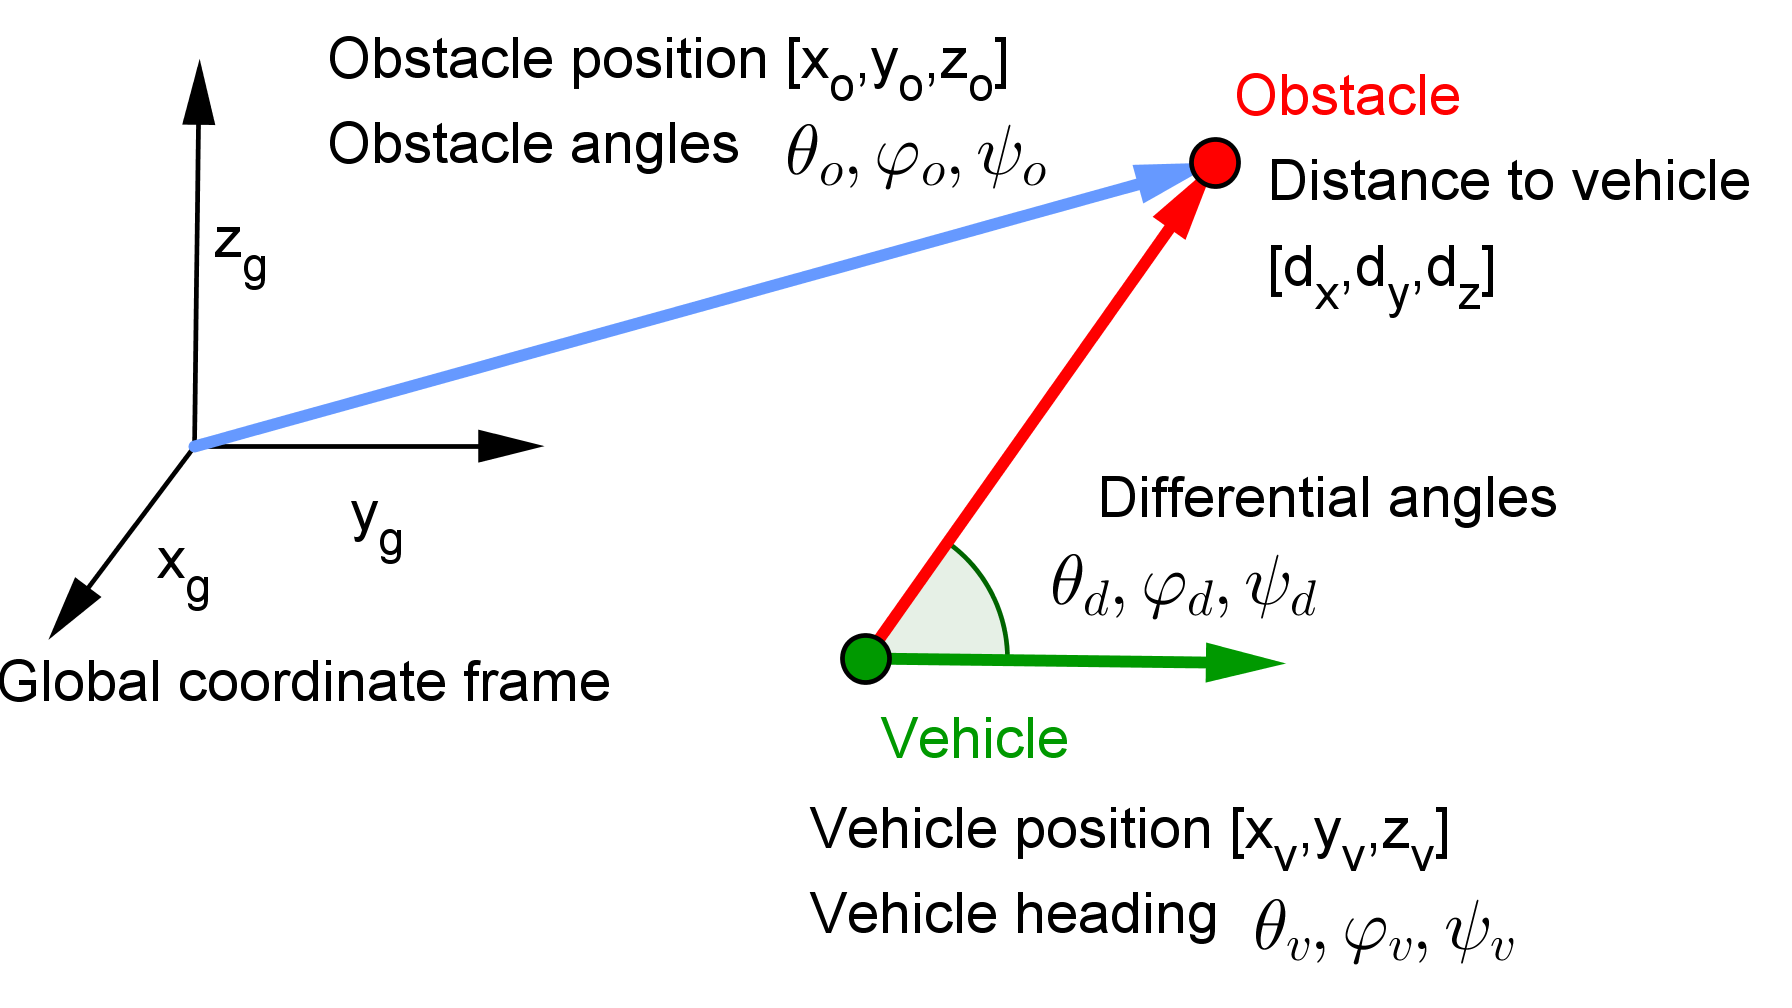
\includegraphics[width=0.55\linewidth]{\FIGDIR/63_Obstacle_Representation.png}
    \caption{Obstacle representation in $3D$ environment.}
    \label{fig:63ObstacleRepresentation}
\end{figure}

\noindent Where $[x_p,y_p,z_p]$ represents global coordinates of obstacle in known world $\mathscr{F}_{3D}$ , angles $\alpha,\beta,\gamma$ represents offset angles at YZ,XZ,XY, planes, differential angles $\delta_\alpha,\delta_\beta,\delta_\gamma$ represents angles definitions between orientation angles of plane $\alpha_v,\beta_v\gamma_v$, $do$ is distance to obstacle and $danger$ represents danger level\\
\newpage\noindent Distance $d_o$ is calculated as norm between obstacle position and vehicle position in global coordinate system, by following equation:
    \begin{equation}
        d_o = \norm{[x_o,y_o,z_o]^T-[x_v,y_v,z_v]^T}
    \end{equation}
Offset angles are calculated based on vehicle and obstacle position by following equations:
    \begin{equation}
        \alpha=\textnormal{atan2}(y_o-y_v,x_o-x_v)
    \end{equation}
    \begin{equation}
        \beta=\textnormal{atan2}(z_o-z_v,x_o-x_v)
    \end{equation}
    \begin{equation}
        \gamma=\textnormal{atan2}(z_o-z_v,y_o-y_v)
    \end{equation}
Differential angles are calculated based on vehicle orientation angles and obstacle offset angles, by following equations:
    \begin{equation}
        \delta_\alpha = \textnormal{atan2}(\sin(\alpha-\alpha_v),\cos(\alpha-\alpha_v))
    \end{equation}
    \begin{equation}
        \delta_\beta = \textnormal{atan2}(\sin(\beta-\beta_v),\cos(\beta-\beta_v))
    \end{equation}
    \begin{equation}
        \delta_\alpha = \textnormal{atan2}(\sin(\gamma-\gamma_v),\cos(\gamma-\gamma_v))
    \end{equation}
Danger level is calculated based on safety margin $s_m$, if $s_m$, if $d_o \ge s_m$ danger does not exist, otherwise if $\abs{\delta_\alpha} \le \pi, \abs{\delta_\beta} \le \pi, \abs{\delta_\gamma} \le \pi $ then direct hit danger is approaching otherwise turn hit danger is approaching. Danger level assessment function is defined in following equation:
    \begin{equation}
        danger = 
        \begin{cases}
            0:&d_o \ge s_m\quad\textnormal{ no danger}\\
            1:&d_o < s_m \textnormal{ and } \delta_\alpha,\delta_\beta,\delta_\gamma\in <-\pi/2,\pi/2> \\&\textnormal{direct hit danger}\\
            2:&d_o < s_m \quad\textnormal{ turn hit danger}\\
        \end{cases}
    \end{equation}

\end{definition}

\section{Control strategy}\label{sec:3DcontrolSimplisticStrategy}
\noindent Main purpose of control strategy is to define discrete set of moves which can be later used in approximation models. Therefore vehicle velocity is set to constant speed $v_v = 1\quad m/s$ because increasing and decreasing speed can make predicted trajectories malformed. It is needed to distinguish between \textit{control strategy} $\Omega(t)$ and \textit{control set} $U(t)$. \textit{Control set} $U(t)$ contains all available control inputs regardless vehicle state and surrounding. \textit{Control strategy} $\Omega(t)$ contains only control inputs $\omega(t)$ which keeps vehicle in safe invariant reachable set $\mathscr{R}$.
\begin{equation}\label{simple3dControlSet}
    u(t)\in U(T) =
    \begin{cases}
        \left [ v_c,0,0,0 \right ]^T & :s_0 \quad\textnormal{fly straight} \\
        \left [ v_c,0,\frac{\pi}{12},0 \right ]^T & :s_1 \quad\textnormal{fly downward} \\
        \left [ v_c,0,-\frac{\pi}{12},0 \right ]^T & :s_2 \quad\textnormal{fly upward} \\
        \left [ v_c,0,0,\frac{\pi}{12} \right ]^T & :s_3 \quad\textnormal{fly left} \\
        \left [ v_c,0,0,-\frac{\pi}{12} \right ]^T & :s_4 \quad\textnormal{fly right} 
    \end{cases}
\end{equation}
Control set $U(t)$ (\ref{simple3dControlSet}) contains five basic movement which affects yaw or pitch angular velocity. This allows us to develop movement set containing basic movement like fly straight, fly upward, fly downward, fly left and fly right. Movement set  is designed to cover maximum maneuverability. From viewpoint of reachable control set $U(t)$ have maximal maneuverability subset $\Gamma(t)$ which contains only maneuvers which are on border of reach set. Maximal maneuverability subset $\Gamma(t)$ is equal to control set $U(t)$ in this case. For example les sharp turn to right $u(t)=\left [ v_c,0,0,-\frac{\pi}{16} \right ]^T$ will be member of control set $U(t)$, but will not be member of maximal maneuverability set $\Gamma(t)$, because there exist sharper turn to right $u(t) = \left [ v_c,0,0,-\frac{\pi}{12} \right ]^T $. Maximal maneuverability set $\Gamma(t)$ is used in estimation of invariant safe reach set $\mathscr{R}$.

\section{Path finding in known environment}\label{ch:pathfindingInKnownEnviroment}
\noindent Abstractly, this is a constrained optimization problem where a feasible
trajectory $(x(t),u(t))$ that minimizes the cost function is found (\ref{eq:costFunction})
\begin{equation}\label{eq:costFunction}
    J =  L(x(t),u(t)) + V(x(T))
\end{equation}
The term $L(x,u)$ is referred to as the integral cost and V $(x(T))$ is the final (or terminal) cost. Definition of integral cost is simple it is summation of trajectory which have been flew, therefore integral cost is defined as trajectory flew in given time is defined by equation (\ref{eq:integral_cost})
\begin{equation}\label{eq:integral_cost}
    L(x(t),u(t)) = \int \norm{[\dot{x}_v(\tau),\dot{y}_v(\tau),\dot{z}_v(\tau)]^T}\quad d\tau
\end{equation}
Terminal cost function $V(x(T))$ must reflect penalization for not reaching goal waypoint. These functions are usually defined in form of penalty $\times$ coefficient, penalty can be seen as remaining shortest distance to goal (\ref{eq:distanceToGoalCalc}). Crashing to obstacle is penalized by $d_g$, when crash is inevitable $d_g=\infty$. Coefficient for final cost will be formulated as penalization function of vehicle orientation ($\alpha_v,\beta_v,\gamma_v$) and vector defined by start waypoint $\mathscr{W}_S$ and goal waypoint $\mathscr{W}_G$. The biggest difference between planar angles in absolute value is 180 degrees or $\pi$ radians. 
\begin{equation}\label{eq:penalizationCoeficient}
    \begin{aligned}
    p(\alpha_v,\beta_v,\gamma_v,\mathscr{W}_S,\mathscr{W}_G)= 1 +&\\
    +&\frac{\abs{\alpha_v -   \textnormal{atan2}(z_{\mathscr{W}_G}-z_{\mathscr{W}_S},y_{\mathscr{W}_G}-y_{\mathscr{W}_S})}}{\pi}\\
    +&\frac{\abs{\beta_v -   \textnormal{atan2}(z_{\mathscr{W}_G}-z_{\mathscr{W}_S},x_{\mathscr{W}_G}-x_{\mathscr{W}_S})}}{\pi}\\
    +&\frac{\abs{\alpha_v -   \textnormal{atan2}(y_{\mathscr{W}_G}-y_{\mathscr{W}_S},x_{\mathscr{W}_G}-x_{\mathscr{W}_S})}}{\pi}\\
    \end{aligned}
\end{equation}
Penalisation coefficient is given by (\ref{eq:penalizationCoeficient}) and with range $p(\dots)\in [1,4]$, therefore terminal cost of state in time $T$ can be given by equation (\ref{eq:terminalCost}).
\begin{equation}\label{eq:terminalCost}
    V(x(T)) = \int_{t_0}^\tau \dot{x}(s) +\dot{y}(s)+\dot{z}(s) ds + \norm{\begin{bmatrix}x(T)-x(\tau)\\y(T)-y(\tau)\\z(T)-z(\tau)\\ \end{bmatrix}}
\end{equation}
Terminal cost is represented as traveled path distance and direct distance to goal point $[x(T),y(T),z(T)]$ in time $\tau$.
\begin{figure}[H]
    \centering
    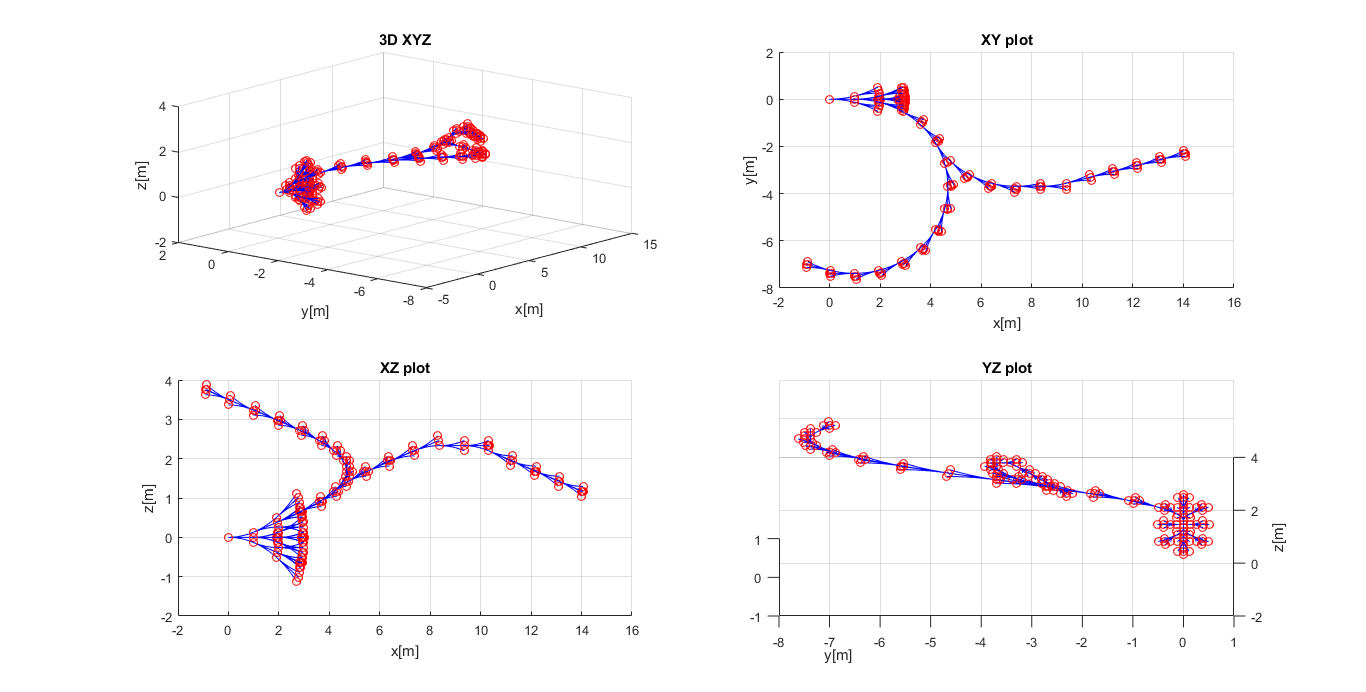
\includegraphics[width=0.75\linewidth]{\FIGDIR/58_Rapid_exploration_path_tree.png}
    \caption{Rapid path exploration tree example with weighted expand cost function $J^*$.}
    \label{fig:58rapidPathExploaation}
\end{figure}
\noindent Rapid path exploration method is method for finding feasible paths in known environment based on limited system dynamics $\dot{x}=f(x,u)$ where input belongs to control  set $u(t)\in U(T)$, example can be seen in figure \ref{fig:58rapidPathExploaation}.

Algorithm is based on tree search of possible movement nodes which represents vehicle state snapshots $x(t_i) i\in \N^+$. State snapshots are calculated based on predictive or linear model, to save computation time and calculation guarantees that real vehicle state $\hat{x}(t_i)$ will reach predicted state $x(t_i)$ with small perturbation $\epsilon$ therefore for each predicted state following inequality holds:
\begin{equation}\label{eq:marginalErrorofPrediction}
    \norm{\hat{x{t_i}}-x(t_i)}\le \epsilon^i,\quad i \in \N^+
\end{equation}
All possible paths $p$ in search tree are represented as sequence of nodes. Each node have defined parent, which is reference to previous node and leafs which are references to possible followers in path. For our purpose augmented data structure \textit{Node} will be presented with following properties:
\begin{enumerate}
    \item \textit{Movement} - movement which has been executed on this node.
    \item \textit{Goal distance} - distance to goal point in space calculated by (\ref{eq:distanceToGoalCalc}).
    \item \textit{Explored} - indication if node have been explored by stack execution true or false.
    \item \textit{Vehicle} - vehicle structure with state and obstacles situation.
    \item \textit{Parent} - parent node handle, if empty node is root of tree. 
    \item \textit{Leafs} - list of accessible non vehicle destructive leafs.
\end{enumerate}
\begin{equation}\label{eq:distanceToGoalCalc}
    d_{goal}(vehicle,\mathscr{W}_g) = 
    \begin{cases}
        \norm{\vec{x}_v-\vec{x}_{goal}}&:\nexists o \in \mathscr{O}; o.danger = 1 \vee 2\\
        \infty&:otherwise
    \end{cases}
\end{equation}
For purpose of rapid exploration limited move set needs to be introduced, therefore based on defined simplistic system model control set (\ref{simple3dControlSet}):
\begin{equation}\label{eq:rapidExplorationMovementSet}
    moveSet=
    \begin{cases}
        \left\{straight,left,right,up,down \right\} &: node.movement == straight\\
        \left\{straight,left, \right\} &: node.movement == left\\
        \left\{straight,right \right\} &: node.movement == right\\
        \left\{straight,up \right\} &: node.movement == up\\
        \left\{straight,down \right\} &: node.movement == down
    \end{cases}
\end{equation}
Goal of rapid exploration is to cover maximum amount of space without redundancy therefore allowed movement set \ref{eq:rapidExplorationMovementSet} is covering this situation. For example movement series $[right,left]$ returns to path given by movement series $[straight,straight]$, therefore possible movements after i finis $right$ movement are $right,straight$. This rule reduces search tree complexity from branching factor $n^5$ to branching factor $n^3$. Expand function represented by algorithm \ref{alg:03}.
\\
\begin{algorithm}[H]
\caption{Node expand(...) function.}
\label{alg:03}
\SetKwInOut{Input}{Input}\SetKwInOut{Output}{Output}
\Input{Node node}
\Output{Node[] leafs}
\If{isEmpty(node.leafs)}{
    \ForEach{$appliedMovement\in \left\{straight,left,right,up,down \right\}$}{
        newVehicle = vehicle.predictPosition(appliedMovement);\\
        Node child = new Node(vehicle);\\
        child.recalculateDistance();\\
        child.parrent = node;\\
        node.leafs.append(child);
    }
}
\end{algorithm}
Node selection is executed based on algorithm \ref{alg:04}. Not all leafs of expanded node can be exploration candidates, because some movements can lead to vehicle crash, which is represented by $node.goalDistance = \infty$. Other reason to decline leaf as exploration candidate is inappropriate movement, movement set which is based on parent node movement (\ref{eq:rapidExplorationMovementSet}), can allow only certain candidates to be explored. Other selection criteria based on system dynamics or constraints can be introduced into selection function later.

\begin{algorithm}[H]
    \caption{Node select(...) function.}
    \label{alg:04}
    \SetKwInOut{Input}{Input}\SetKwInOut{Output}{Output}
    \Input{Node node}
    \Output{Node[] candidates}
    candidates = [];\\
    \ForEach{leaf $\in$ node.leafs}{
    \If{leaf.movement $\in$ moveSet and leaf.goalDistance $\neq \infty$ and\\
        leaf.goalDistance $\le$ node.goalDistance and leaf.explored == false}{
            leaf.explored = true;\\
            candidates.append(leaf);
    }
}
\end{algorithm}
\newpage\noindent  Stack structure search is used for heuristic search of optimal path according to cost function (\ref{eq:costFunction}). Path given by heuristic algorithm \ref{alg:05}. is semi-optimal strongly depending on chosen time interval $t_i$ for prediction, count of predicted states $i$ and acceptable marginal error of prediction (\ref{eq:marginalErrorofPrediction}). Nevertheless its very fast and stable, and with limited search dynamics can cover large quantity of space, which makes it ideal candidate for obstacle avoidance in known environment. 

\begin{algorithm}[H]
    \caption{Search path function.}
    \label{alg:05}
    \SetKwInOut{Input}{Input}\SetKwInOut{Output}{Output}
    \Input{Node root, $\mathscr{WP}$ goal}
    \Output{Node path}
    stack = [root];
    \While{~isEmpty(stack)}{
        node = findBestCandidate(stack,goal); (\ref{eq:costFunction})\\
        node.expand($\dots$); (alg. \ref{alg:03}.)\\
        candidates = node.select($\dots$); (alg. \ref{alg:04}.)\\
        \ForEach{candidate $\in$ candidates}{
            \If{candidate.distance(goal) $\le$ marginDistance}{
                return candidate;
            }
        }
    }
\end{algorithm}

\section{Movement automaton predictor}\label{ch:movementAutomatonPredictor}
\noindent Vehicle system is given by model from section \ref{sec:3DsimplisticplaneModel}. Vehicle control is defined as movement automation $\mathscr{MA}$ with rapid exploration movement set defined in equation \ref{eq:rapidExplorationMovementSet}. Path exploration approach is given in section. 
\ref{ch:pathfindingInKnownEnviroment}. Movement predictor needs to be developed in order to obtain control signal $u(t)$ It is possible to predict movement buffer $B_{\mathscr{MA}}$, between vehicle initial position $x_0$ and waypoint, when known obstacle set $\mathscr{O}$ is given and movement state can be predicted for chain of movements. This approach have been defined in alg. \ref{alg:05}. as rapid exploration tree. Vehicle state $x(t_0)$ at start of mission execution is known. Vehicle state in discrete time $x(t)$ is given by equation \ref{eq:vehicleStateDiscreteKnown}. Where $x_v(t),y_v(t),z_v(t)$ is vehicle position in local coordinate frame and $\alpha_v(t),\beta_v(t),\gamma_v(t)$ is vehicle orientation angles.
\begin{equation}\label{eq:vehicleStateDiscreteKnown}
    x(t) = [x_v(t),y_v(t),z_v(t),\alpha_v(t),\beta_v(t),\gamma_v(t)]^T;
\end{equation}
Base movement table for movements $m_i(1)\in M$ have been measured on system model (\ref{sec:3DsimplisticplaneModel}). This table represents vehicle position and orientation differences after execution of movement. Vehicle initial state was set at center of local coordinate frame with narrow orientation $[x_0,y_0,z_0]=[0,0,0]$. Vehicle initial orientation was aligned with main frame axis X, therefore initial orientation angles are $[\alpha_0,\beta_0,\gamma_0] = [0,0,0]$. Vehicle velocity was set to constant value $v_v = 1 ms^{-1}$. Vehicle position after movement execution is given by parameters $x_b,y_b,z_b$ at time $t+1$. Vehicle orientation is given by parameters $\alpha_b,\beta_b,\gamma_b$. Givem parameters are also absolute shifting, because initial state is $[x_0,y_0,z_0,\alpha_b,\beta_b,\gamma_b]$ set to $\vec{0}$.
\begin{table}[H]
    \centering
    \begin{tabular}{|l||c|c|c|c|c|}
    \hline
        $v_x/m_i$           &    Straight $\circledcirc$ & Down $\Downarrow$  & Up $\Uparrow$    & Left $\Leftarrow$ & Right $\Rightarrow$\\\hline\hline
        $x_b [m]$           &    1.00	  & 0.98  & 0.98  & 0.98 & 0.98\\\hline
        $y_b [m]$           &    0	      & 0	  & 0	  & 0.13 & -0.13\\\hline
        $z_b [m]$           &    0	      & -0.13 & 0.13  &	0	 & 0\\\hline
        $\alpha_b [rad]$	&    0	      & 0	  & 0	  & 0    & 0\\\hline
        $\beta_b [rad]$     &    0	      & 0.2   & -0.26 & 0	 & 0\\\hline
        $\gamma_b [rad]$    &    0	      & 0	  & 0	  & 0.26 & -0.26\\\hline
    \end{tabular}
    \caption{Base values for movement application, vehicle position difference $x_v,y_v,z_v$ and orientation differences $\alpha_v,\beta_v,\gamma_v$.}
    \label{tab:movementPredictor}
\end{table}
\noindent With defined base movement table (tab. \ref{tab:movementPredictor}). with defined shifting for movement at time $t_0+1$, \textit{rotation} (\ref{eq:rotationSimplisticPredictor}) and \textit{shifting} (\ref{eq:shiftingSimplisticPredictor}) equations must be defined in order to obtain predicted position $\hat{x}(t+1)$. Position after movement execution $[\hat{x}(t+1),\hat{y}(t+1),\hat{z}(t+1)]$ is depending on vehicle orientation before movement execution $[\alpha_v(t),\beta_v(t),\gamma_v(t)]$. Rotation function rotates vehicle position $[x_b(t_0),y_b(t_0),z_b(t_0)]$ according to vehicle orientation angles $[\alpha_v(t),\beta_v(t),\gamma_v(t)]$. For rotation standard rotation matrix $R_{XYZ}(\alpha,\beta\gamma)$ (\ref{eq:xyzspaceRotationMatrix}) is used. Final position offset vector $[\tilde{x}_b(t+1),\tilde{y}_b(t+1),\tilde{z}_b(t+1)]$ at predicted time $t+1$ is given by equation \ref{eq:rotationSimplisticPredictor}.
\begin{equation}\label{eq:rotationSimplisticPredictor}
    \begin{bmatrix}
        \tilde{x}_b\\ 
        \tilde{y}_b\\
        \tilde{z}_b\\
    \end{bmatrix}
    = R_{XYZ}(\alpha_v(t),\beta_v(t),\gamma_v(t))
    \begin{bmatrix}
        x_b\\ 
        y_b\\
        z_b\\
    \end{bmatrix}
\end{equation}
Predicted state vector $\hat{x}(t+1)$ a at time $t+1$ is obtained by combining position offset vector $[\tilde{x}_b(t+1),\tilde{y}_b(t+1),\tilde{z}_b(t+1)]$, orientation offset vector $\alpha_b(t+1),\beta_b(t+1),\gamma_b(t+1)$. as given in equation \ref{eq:shiftingSimplisticPredictor}.
\begin{equation}\label{eq:shiftingSimplisticPredictor}
    \begin{aligned}
    \hat{x}(t+1) & = [\hat{x}_v(t+1),\hat{y}_v(t+1),\hat{z}_v(t+1),\hat{\alpha}_v(t+1),\hat{\beta}_v(t),\hat{\gamma}_v(t)]^T\\
    \hat{x}_v(t+1) & = x_v(t)+\tilde{x}_b\\
    \hat{y}_v(t+1) & = y_v(t)+\tilde{y}_b\\
    \hat{z}_v(t+1) & = z_v(t)+\tilde{z}_b\\
    \hat{\alpha}_v(t+1) & = \alpha_v(t) + \alpha_b\\
    \hat{\beta}_v(t+1) & = \beta_v(t) + \beta_b\\
    \hat{\gamma}_v(t+1) & = \gamma_v(t) + \gamma_b
    \end{aligned}
\end{equation}
Movement automaton $\mathscr{MA}$ has chaining property, therefore movement prediction chaining is also possible via recursive procedure for discrete execution time $t_i$. There exist predicted movement buffer $\hat{B}$ with ordered movement sequence $m_1(1),\dots,m_i(1)$, vehicle state after applying movement $m_{i+1}$ at time $t_i$ can be obtained via equation \ref{eq:discretePredictionChaining}.
\begin{equation}\label{eq:discretePredictionChaining}
    \hat{x}(t_i+1) = f(\hat{x}(t_i),m_{i+1}(1))
\end{equation}
Prediction function $f(\hat{x}(t_i),m_{i+1}(1))$ is in this case function defined by equation \ref{eq:shiftingSimplisticPredictor}, where parameters $[x_b,y_b,z_b,\alpha_b,\beta_b\gamma_b]$ are selected based on movement $m_{i+1}(1)$ type from lookup table  \ref{tab:movementPredictor}.



\chapter{Simulation results}\label{ch:simulationResults}
\noindent This chapter summarizes defines \textit{Virtual playground} where MPC approach was tested. Other sections summarizes simulation results, taking into account: obstacle avoidance (safety margin), control quality (prediction deviation).
\section{Playground definition}\label{ch:3DPlaygroundDefinition}
\noindent For purpose of new theorem formulation, new playground (\ref{fig:new3DPlayground})with added dimension needs to be introduced. Additional element of \textit{mission control} needs to be introduced, because previous experiments was with not coordinated flight and for real missions some coordinated flight is required, therefore waypoint set $\mathscr{WP}$ is added into playground. 
\begin{figure}[H]
    \centering
    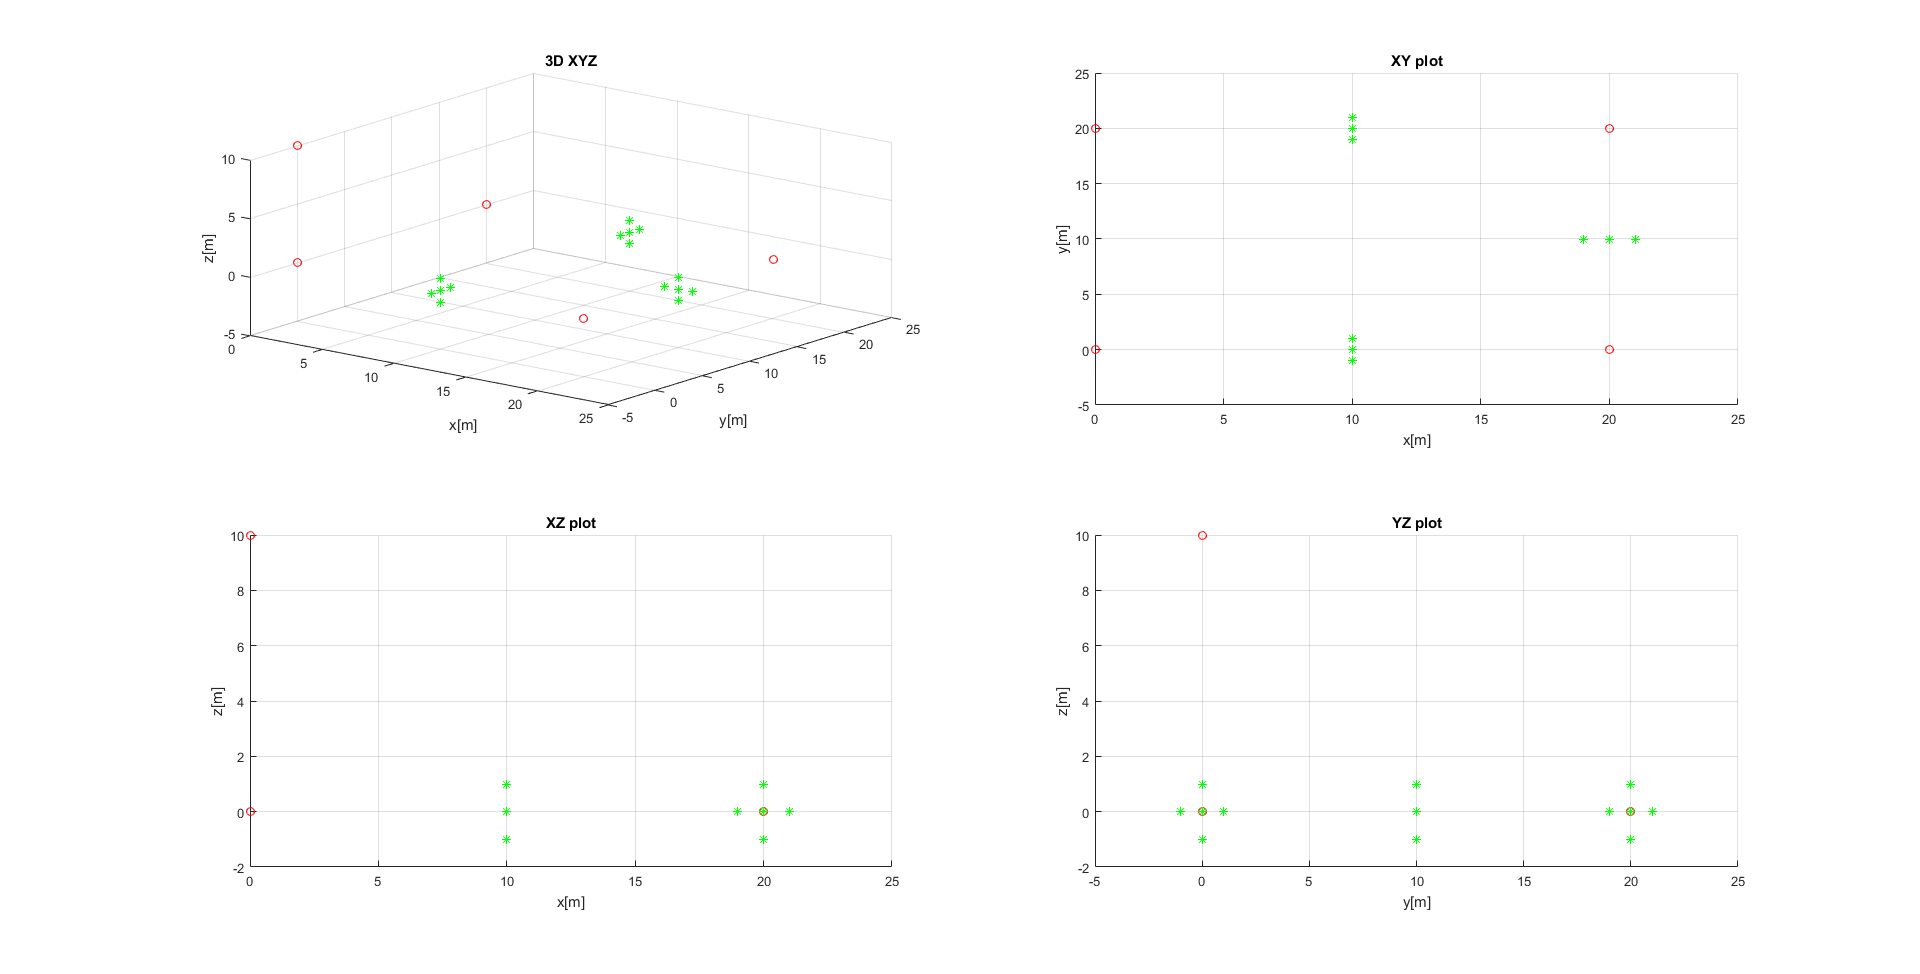
\includegraphics[width=\linewidth]{\FIGDIR/37_Playground_3D.png}
    \caption{Initial playground for obstacle avoidance and optimal path finding testing}
    \label{fig:new3DPlayground}
\end{figure}
\newpage\noindent Waypoint set $\mathscr{WP}$ (\ref{eq:playground3DSimpleWPSet}) contains five waypoins in Cartesian coordinates $\mathscr{WP}_i =[x,y,z]^T$. This set is simple rectangular flight around rectangle with side of 20 meters and slightly elevated end by 10 meters $\mathscr{WP}_E$.

\begin{equation}\label{eq:playground3DSimpleWPSet}
    \begin{aligned}
          \mathscr{WP} = \{ \mathscr{WP}_S &=[0,0,0]^T,\\
                            \mathscr{WP}_1 &=[20,0,0]^T,
                            \mathscr{WP}_2 =[20,20,0]^T,\\
                            \mathscr{WP}_3 &=[0,20,0]^T,
                            \mathscr{WP}_E =[0,0,10]^T,\}
    \end{aligned}
\end{equation}
\noindent Each path tracking algorithm needs to have stop condition which indicates when vehicle should stop following presented waypoint. Usually unit ball stop condition is used (\ref{eq:stopFunctionUnitBall}) where $[x_v,y_v,z_v]^t$ is vehicle position, $[x_g,y_g,z_g]^T$ is waypoint position and $p_t$ is precision threshold.
\begin{equation}\label{eq:stopFunctionUnitBall}
    \norm{\begin{bmatrix}x_g-x_v\\y_g-y_v\\z_g-z_v\end{bmatrix}} \le p_t
\end{equation}
Complete obstacle definition with associated structure can be found in section \ref{s:3dObstacleRepresentationSimplistic}. Single obstacle $o_i\in\mathscr{O}$ is defined by its position $o=[x_o,y_o,z_o]^T$. All obstacles are stored in single obstacle structure $\mathscr{O}$ defined by (\ref{eq:3dSimplisticPlaygroundO}).
\begin{equation}\label{eq:3dSimplisticPlaygroundO}
    \mathscr{O} = \{\mathscr{O}_1,\mathscr{O}_2,\mathscr{O}_3\}
\end{equation}
Obstacle subset $\mathscr{O}_1$ (\ref{eq:3dSimplisticPlaygroundO1}) is defined between waypoints $\mathscr{WP}_S,\mathscr{WP}_1$.
\begin{equation}\label{eq:3dSimplisticPlaygroundO1}
    \mathscr{O}_1 = \{[10,0,0]^T,[10,1,0]^T,[10,-1,0]^T,[10,0,1]^T,[10,0,-1]^T\}
\end{equation}
Obstacle subset $\mathscr{O}_2$ (\ref{eq:3dSimplisticPlaygroundO2}) is defined between waypoints $\mathscr{WP}_1,\mathscr{WP}_2$.
\begin{equation}\label{eq:3dSimplisticPlaygroundO2}
    \mathscr{O}_2 = \{[20,10,0]^T,[20,10,1]^T,[20,10,-1]^T,[19,10,0]^T,[21,10,0]^T\}
\end{equation}
Obstacle subset $\mathscr{O}_3$ (\ref{eq:3dSimplisticPlaygroundO3}) is defined between waypoints $\mathscr{WP}_2,\mathscr{WP}_3$.
\begin{equation}\label{eq:3dSimplisticPlaygroundO3}
    \mathscr{O}_3 = \{[10,20,0]^T,[10,20,1]^T,[10,20,-1]^T,[10,19,0]^T,[10,21,0]^T\}
\end{equation}

\newpage\section{Obstacle avoidance in known environment}
\noindent This testing scenario shows how predictive control works in known environment, where are obstacles are known prior to flight.

Vehicle system is given by model from section \ref{sec:3DsimplisticplaneModel}. Vehicle control is defined as movement automation $\mathscr{MA}$ with rapid exploration movement set defined in equation \ref{eq:rapidExplorationMovementSet}. Path exploration approach is given in section. 
\ref{ch:pathfindingInKnownEnviroment}. Movement predictor is defined in section \ref{ch:movementAutomatonPredictor}. Following parameters and conditions were applied during simulations:
\begin{enumerate}
    \item Vehicle is occupying the unit-ball $\mathscr{B}$ with diameter $0.30$ m.
    \item \textit{Turning radius} of vehicle is $2$ meters.
    \item \textit{Safety margin} $s_m$ have been decided as unit-ball $\mathscr{B}$ with diameter $0.60$ m
    \item \textit{Movement decision} - movement decision is based on reaching goal waypoint with tolerance $t=1m$ and not breaching safety margin $s_m$.
    \item \textit{Prediction error $e_p$} is not known at this point, because there is no disturbance vector $\vec{w}(t)$.
    \item All \textit{obstacles} are known prior flight and they are stored in vehicle obstacle set $o_i\in\mathscr{O}$.
    \item Movement automaton $\mathscr{MA}$ buffer $B_{\mathscr{MA}}$ is filled with all movements predicted via rapid exploration tree with predictor (\ref{eq:discretePredictionChaining}).
    \item \textit{Obstacle avoidance} algorithm is executed at the beginning of mission.
\end{enumerate}

\noindent Prediction calculation was very fast ($\sim$0.2s), but initial results may be neglected in real system and real environment. Predictor approach is similar to RRT \cite{kuffner2000rrt}, which gives good prepositions for calculation time.

Predicted movements for flight in known environment from $\mathscr{WP}_S$ to $\mathscr{WP}_E$ have follow values: $B_{\mathscr{MA}}$ = \textit{[$\circledcirc$(6), $\Downarrow$(3), $\circledcirc$(1), $\Uparrow$(5), $\circledcirc$(3), $\Downarrow$(1), $\circledcirc$(1), $\Uparrow$(1), $\Leftarrow$(6), $\circledcirc$(1), $\Downarrow$(1), $\circledcirc$(1), $\Uparrow$(1), $\circledcirc$(1), $\Rightarrow$(1), $\circledcirc$(2), $\Downarrow$(2), $\circledcirc$(1), $\Uparrow$(1), $\circledcirc$(1), $\Leftarrow$(1), $\circledcirc$(1), $\Leftarrow$(6), $\circledcirc$(1), $\Uparrow$(2), $\circledcirc$(1), $\Downarrow$(2), $\circledcirc$(1), $\Uparrow$(2), $\circledcirc$(1), $\Rightarrow$(1), $\circledcirc$(2), $\Leftarrow$(7), $\circledcirc$(1), $\Uparrow$(3), $\circledcirc$(1), $\Downarrow$(1), $\circledcirc$(1), $\Uparrow$(1), $\circledcirc$(2), $\Downarrow$(1), $\circledcirc$(1), $\Uparrow$(1), $\circledcirc$(5).]} 

\begin{figure}[H]
    \centering
    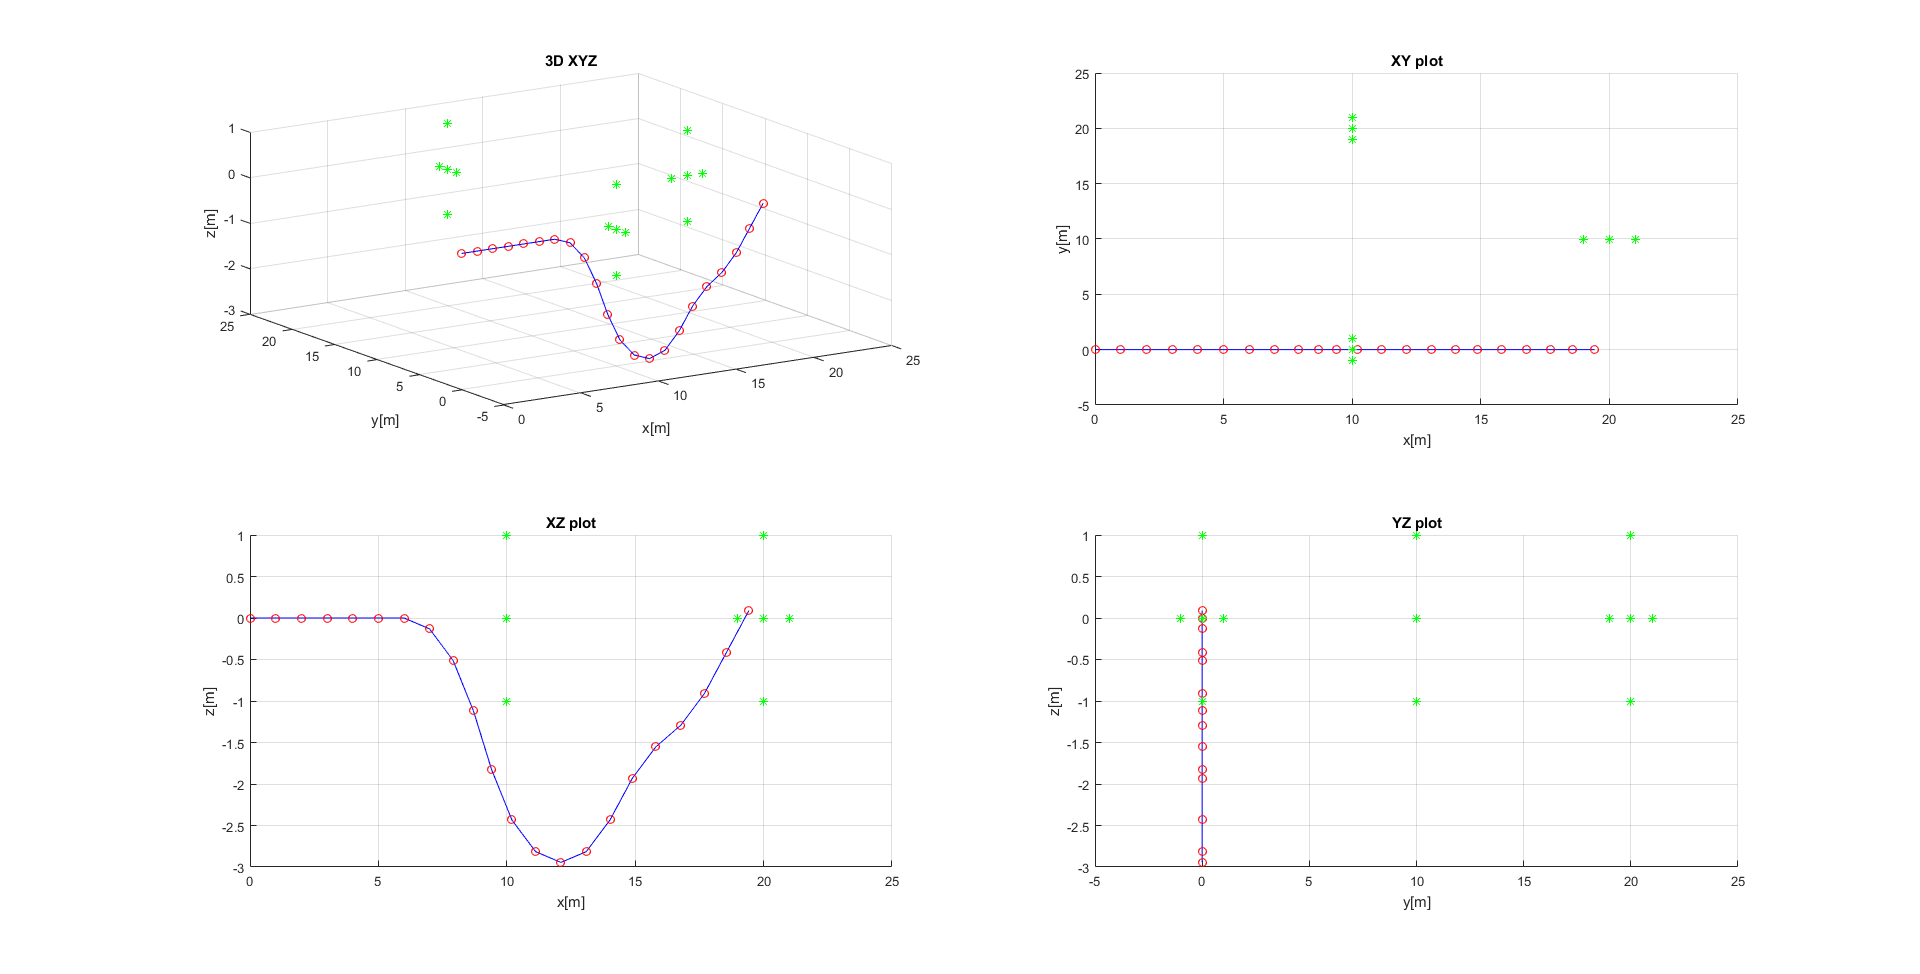
\includegraphics[width=\linewidth]{\FIGDIR/52_First_waypoint_movement.png}
    \caption{First obstacle avoidance at $\mathscr{WP}_1=[20,0,0]^T$.}
    \label{fig:52firstObstacleKnown}
\end{figure}
\noindent Flight between $\mathscr{WP}_S$ to $\mathscr{WP}_1$ was normal and vehicle avoided obstacle choosing bottom path, which is very dangerous in real situation. Real vehicle should choose right,left or top avoidance path in order to minimize collision risks. Decision of rapid exploration algorithm was made, because there is no weight on movement $m_i(t_i)$ in back-stepping calculation process. Trajectory is portrayed in figure \ref{fig:52firstObstacleKnown}. Executed movements during flight from $\mathscr{WP}_S$ to $\mathscr{WP}_1$ have follow values: $B_{\mathscr{MA}}$ = \textit{[$\circledcirc$(6), $\Downarrow$(3), $\circledcirc$(1), $\Uparrow$(5), $\circledcirc$(3), $\Downarrow$(1), $\circledcirc$(1), $\Uparrow$(1)]}. 
\begin{figure}[H]
    \centering
    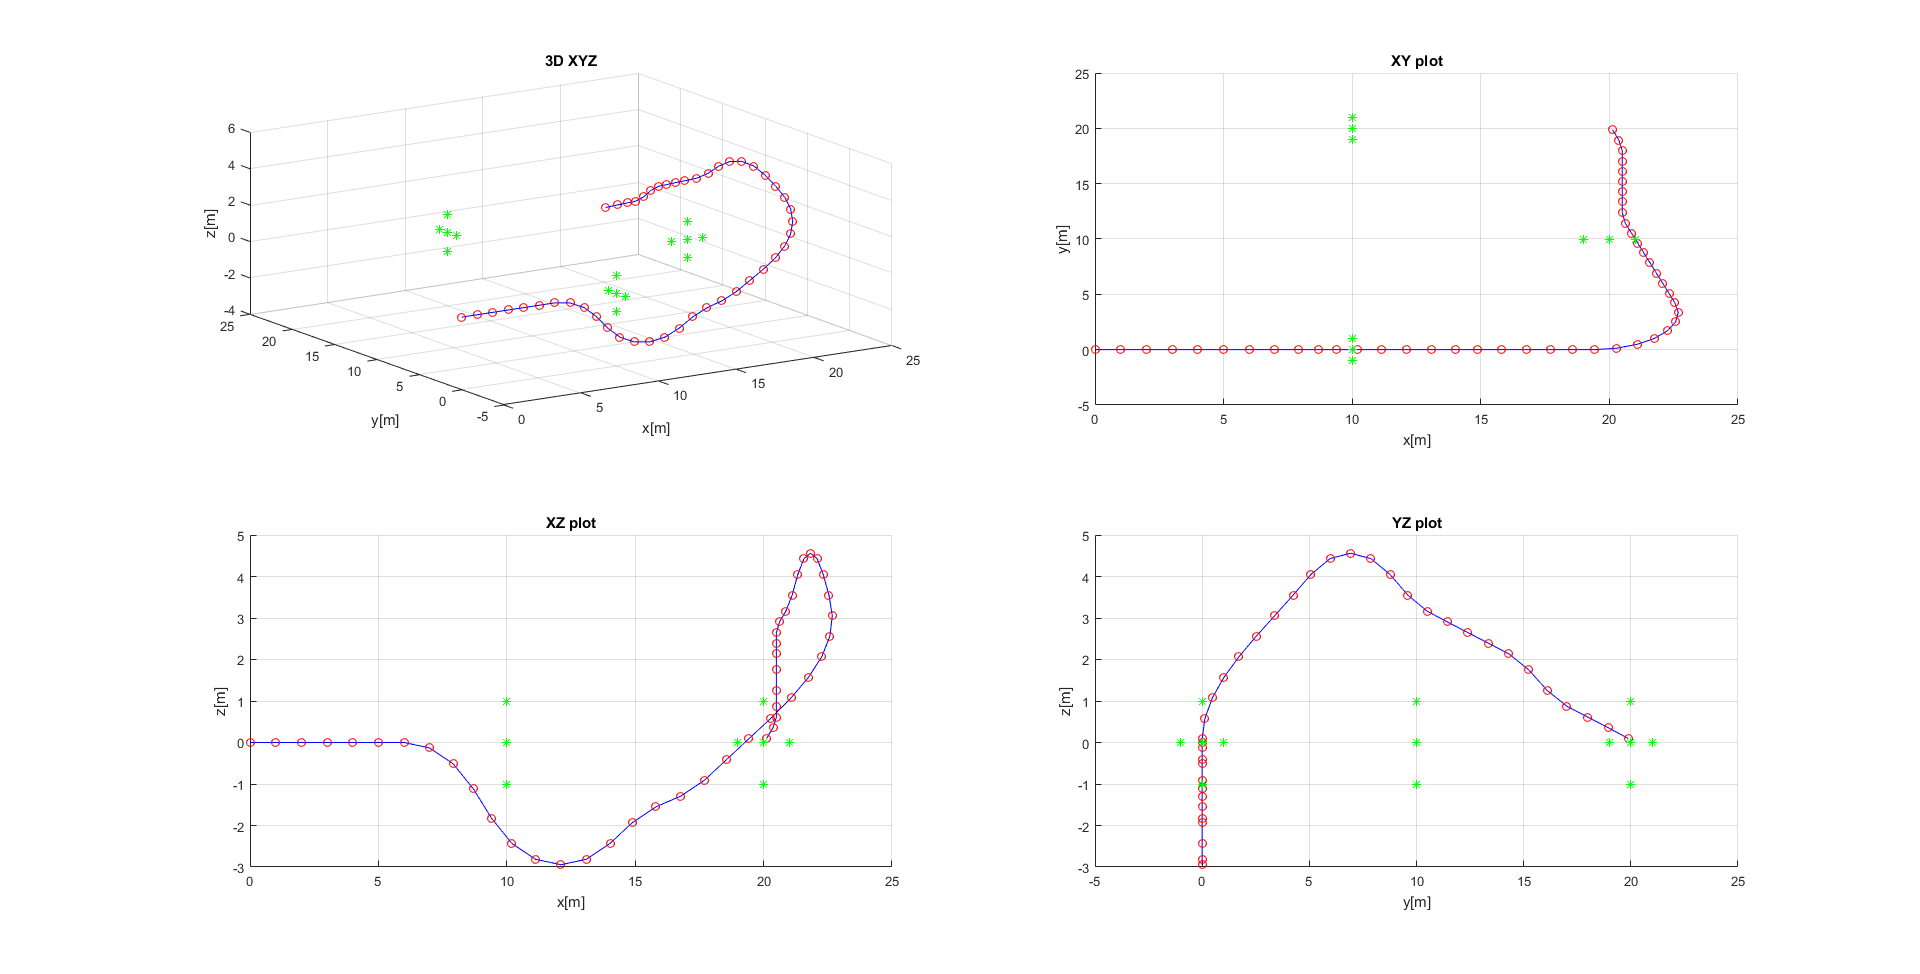
\includegraphics[width=\linewidth]{\FIGDIR/53_Second_waypoint_movement.png}
    \caption{Obstacle avoidance at $\mathscr{WP}_2=[20,20,0]^T$.}
    \label{fig:53secondObstacleKnown}
\end{figure}
\noindent Flight between waypoints $\mathscr{WP}_1$ to $\mathscr{WP}_2$ used top avoidance maneuver, because starting position when obstacle was hindering direct path was a top of obstacle center $o_6=[20,10,0]^T$. Trajectory is portrayed in figure \ref{fig:53secondObstacleKnown}. Executed movements during flight from $\mathscr{WP}_1$ to $\mathscr{WP}_2$ have follow values: $B_{\mathscr{MA}}$ = \textit{[$\Leftarrow$(6), $\circledcirc$(1), $\Downarrow$(1), $\circledcirc$(1), $\Uparrow$(1), $\circledcirc$(1), $\Rightarrow$(1), $\circledcirc$(2), $\Downarrow$(2), $\circledcirc$(1), $\Uparrow$(1), $\circledcirc$(1), $\Leftarrow$(1), $\circledcirc$(1)]}.
\begin{figure}[H]
    \centering
    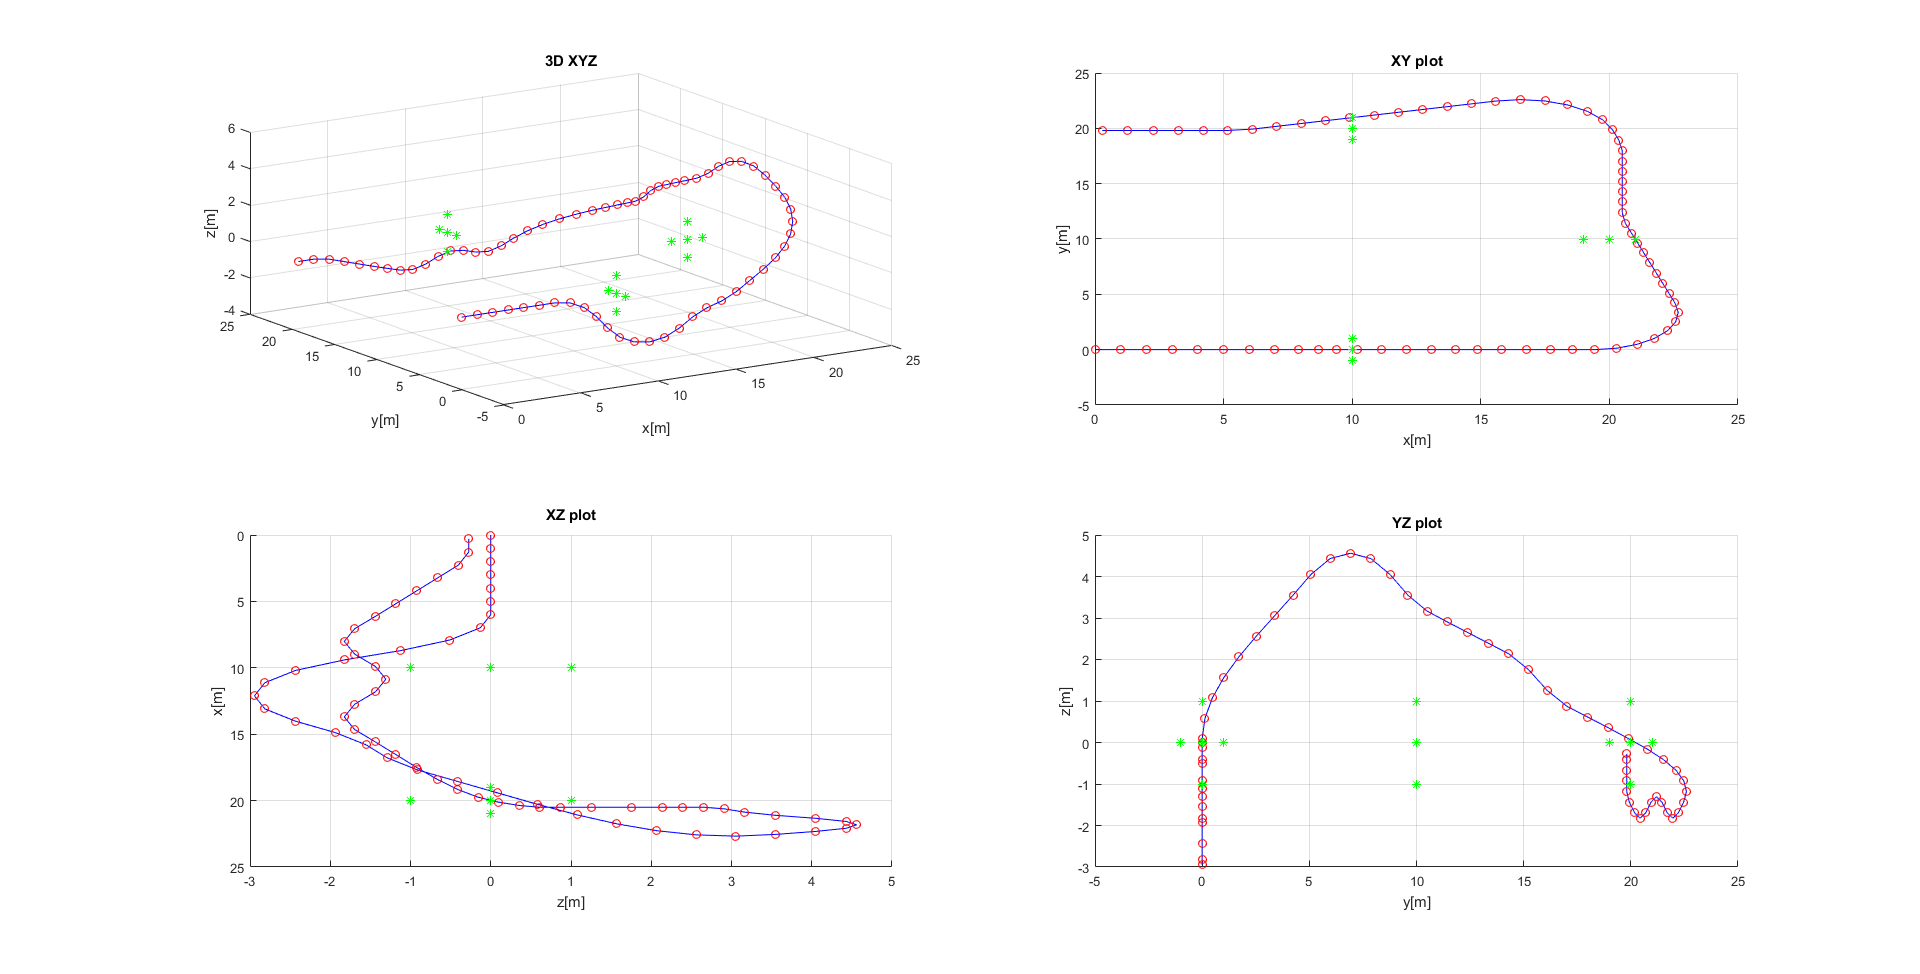
\includegraphics[width=\linewidth]{\FIGDIR/54_Third_waypoint_movement.png}
    \caption{Third obstacle avoidance at $\mathscr{WP}_3=[0,20,0]^T$.}
    \label{fig:54thirdObstacleKnown}
\end{figure}
\noindent Flight between waypoints $\mathscr{WP}_2$ to $\mathscr{WP}_3$ used bottom avoidance maneuver, because starting position when obstacle was hindering direct path was a bottom of obstacle center $o_{11}=[10,20,0]^T$. Trajectory is portrayed in figure \ref{fig:54thirdObstacleKnown}. Executed movements during flight from $\mathscr{WP}_2$ to $\mathscr{WP}_3$ have follow values: $B_{\mathscr{MA}}$ = \textit{[$\Leftarrow$(6), $\circledcirc$(1), $\Uparrow$(2), $\circledcirc$(1), $\Downarrow$(2), $\circledcirc$(1), $\Uparrow$(2), $\circledcirc$(1), $\Rightarrow$(1), $\circledcirc$(2)]}.
\begin{figure}[H]
    \centering
    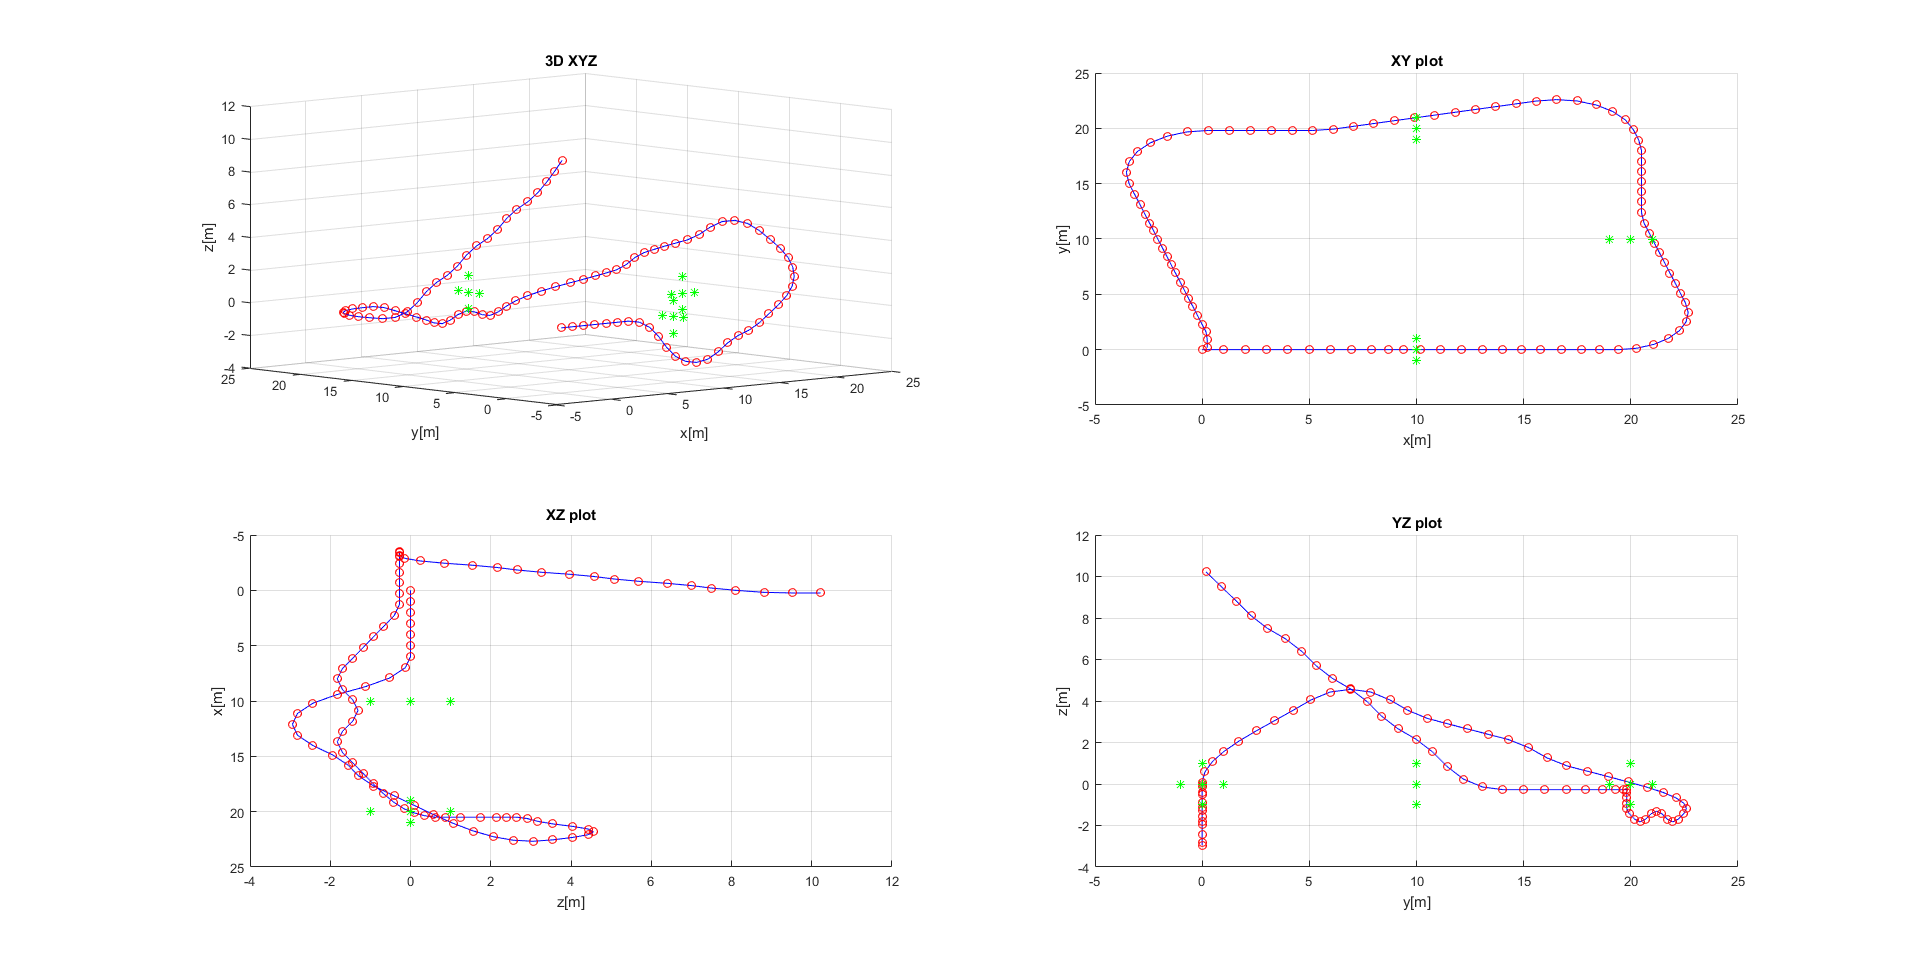
\includegraphics[width=\linewidth]{\FIGDIR/55_Fourth_waypoint_movement.png}
    \caption{Forth waypoint movement at $\mathscr{WP}_4=[0,0,10]^T$.}
    \label{fig:55fourthObstacleknown}
\end{figure}
\noindent Flight between waypoints $\mathscr{WP}_3$ to $\mathscr{WP}_E$ was direct flight between two waypoints until stop condition at $\mathscr{WP}_E$ was triggered. Trajectory is portrayed in figure \ref{fig:55fourthObstacleknown}. Executed movements during flight from $\mathscr{WP}_3$ to $\mathscr{WP}_E$ have follow values: $B_{\mathscr{MA}}$ = \textit{[$\Leftarrow$(7), $\circledcirc$(1), $\Uparrow$(3), $\circledcirc$(1), $\Downarrow$(1), $\circledcirc$(1), $\Uparrow$(1), $\circledcirc$(2), $\Downarrow$(1), $\circledcirc$(1), $\Uparrow$(1), $\circledcirc$(5)]}.
\begin{figure}[H]
    \centering
    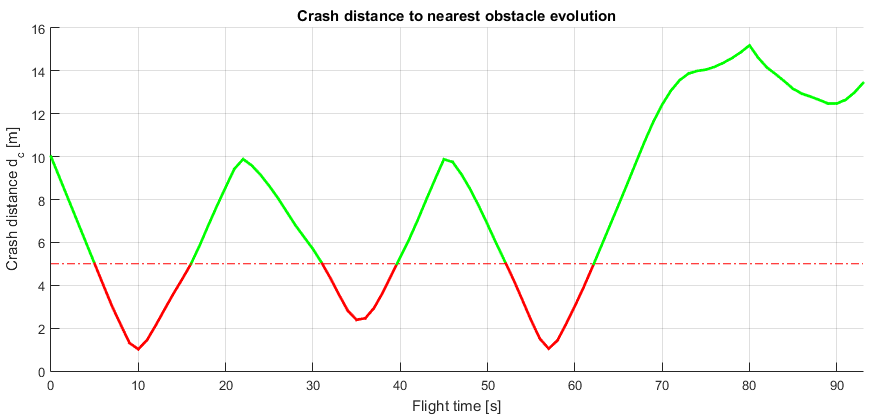
\includegraphics[width=\linewidth]{\FIGDIR/60_Crash_distance_to_nearest_obstacle_evolution_known_world.png}
    \caption{Vehicle crash distance $d_c$ evolution during flight.}
    \label{fig:vehicleCrashDistanceEvolutionKnownWorld}
\end{figure}
\noindent Vehicle crash distance function $d_c$ is vaguely defined as distance to nearest obstacle during time of flight. Crash distance evolution is portrayed in figure \ref{fig:vehicleCrashDistanceEvolutionKnownWorld}. Crash distance $d_c$ was greatest in time of waypoint $\mathscr{WP}_i$ reach, because obstacles $\mathscr{O}$ were positioned in midle between waypoints. Crash distance $d_c$ is divided into two zones:
\begin{enumerate}
    \item \textit{Safe zone} - distance where turn to any direction is possible, this distance is calculated as $2s_m+\mathscr{B}(r)$. In this case was safe distance determined as $5m$.
    \item \textit{Dangerous zone} - distance where turn to any direction is limited. This distance is defined as interval between $B(r)$ and $2s_m+\mathscr{B}(r)$.
\end{enumerate}
Vehicle never breached safety margin $s_m=0.60m$ which is sufficient in this case. Prediction quality is very important factor in predictive control, therefore quantitative measurement for prediction of this system have been introduced (\ref{eq:movementAutomatonPredictionError}). Movement automaton prediction error $e_p$ is based on mean square prediction error (MSE).
\begin{equation}\label{eq:movementAutomatonPredictionError}
    e_p=\sqrt{\sum_{t_i=t_0+i}^{i\in\{1,\dots,n\}} \left (\hat{x}(t_i)-x(t_i)\right)^2}    
\end{equation}

\noindent Movement automaton prediction error compares predicted state $\hat{x}$ and real system state $x$ for each movement execution time $t_i$. Movement execution time in this case was $s_1$ so time $t_i$ was defined as $t_i=t_0+i, i\in\{1,\dots,n\}$, where n is total count of executed movements. Movement automaton prediction error $e_p$ was in this case $e_p\approx 0$.
\begin{figure}[H]
    \centering
    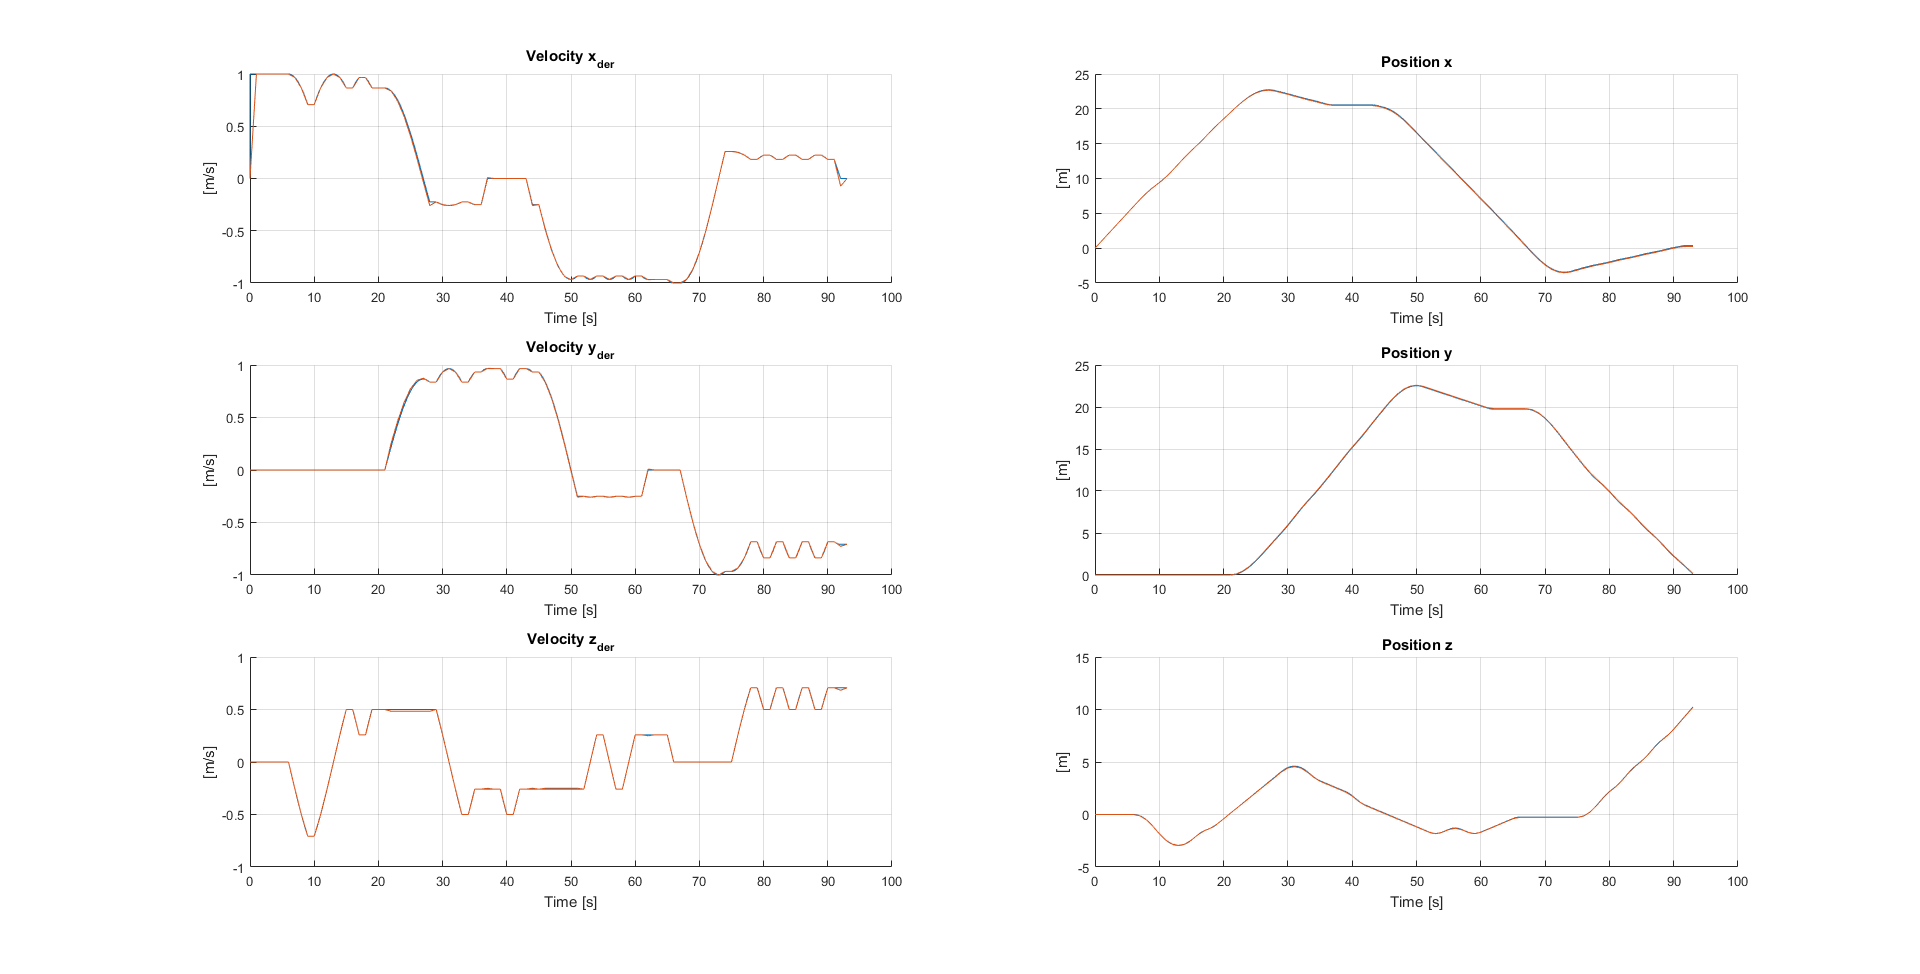
\includegraphics[width=\linewidth]{\FIGDIR/56_Vehicle_position.png}
    \caption{Vehicle position $x,y,z$ and their derivations $\dot{x},\dot{y},\dot{z}$ evolution during flight.}
    \label{fig:vehicleStateKnown1}
\end{figure}
\noindent Vehicle position $x,y,z$ and their derivations $\dot{x},\dot{y},\dot{z}$ and their evolution during flight is portrayed in figure \ref{fig:vehicleStateKnown1}. Brown color is used for predicted model state and blue color is used for real model parameter evolution. Both models are equal, supported by movement automaton prediction error $e_p\approx 0$.
\begin{figure}[H]
    \centering
    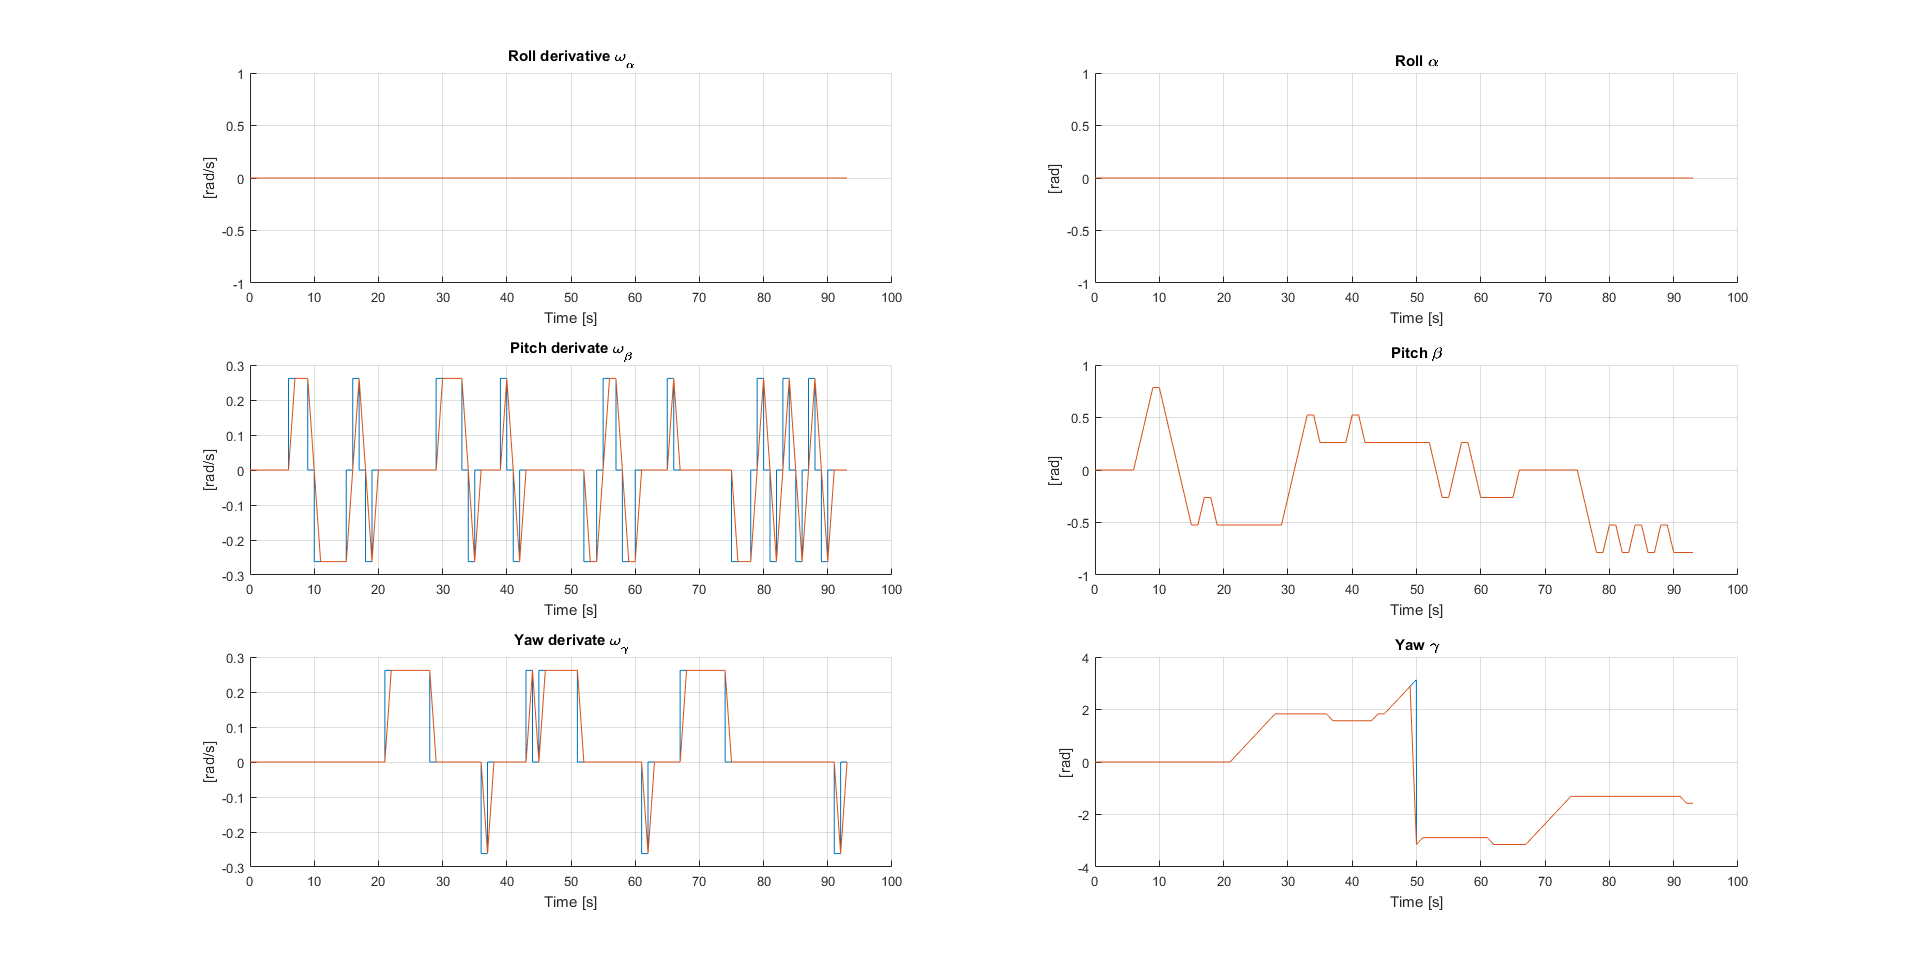
\includegraphics[width=\linewidth]{\FIGDIR/57_Vehicle_angles.png}
    \caption{Vehicle positional angles $\alpha,\beta,\gamma$ and their angular velocities $\omega_\alpha,\omega_\beta,\omega_\gamma$ evolution during flight}
    \label{fig:vehicleStateKnown2}
\end{figure}
\noindent Similar to previous comparison (fig. \ref{fig:vehicleStateKnown1}.) Comparison for vehicle positional angles $\alpha,\beta,\gamma$ and their angular velocities $\omega_\alpha,\omega_\beta,\omega_\gamma$ evolution during flight holds previous assumption (fig. \ref{fig:vehicleStateKnown2}).
\chapter{Conclusion}\label{ch:conclusion}
\noindent This chapter outlines future research heading and discuss quality of MPC control used with movement automaton $\mathscr{MA}$ control.

\section{Summary of simulation}
\noindent Simulation of system $\dot{x}=f(x,\mathscr{MA})$ show that MPC controller is feasible for plant (\ref{eq:simple3ddifferentialequations}) control.  
\begin{figure}[H]
    \centering
    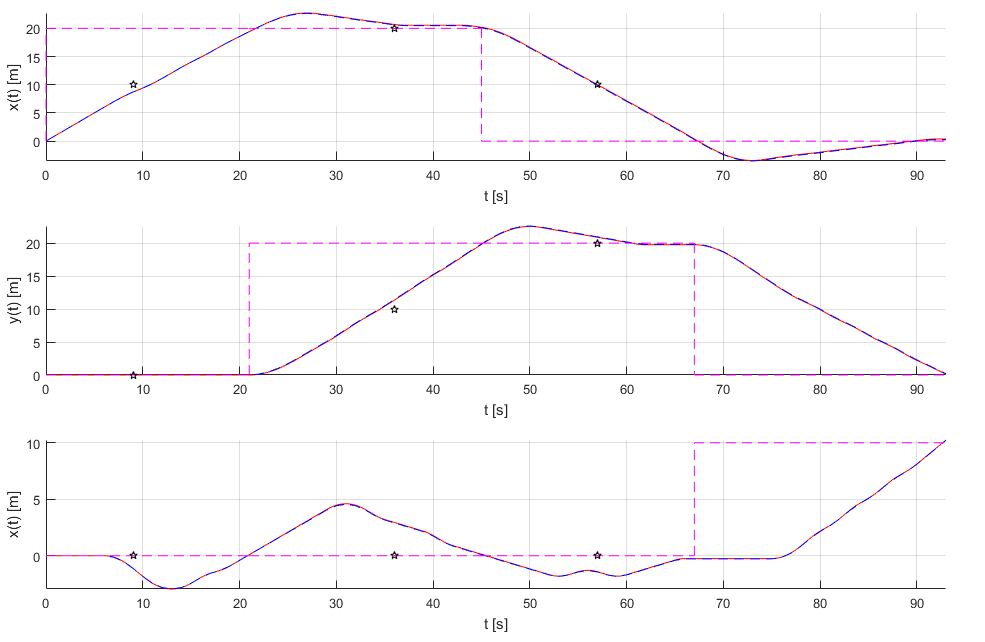
\includegraphics[width=\linewidth]{\FIGDIR/74_MPC_Performance.png}
    \caption{MPC performance at trajectory tracking $[x(t),y(t),z(t)]$.}
    \label{fig:mpcPerformance}
\end{figure}
\noindent Predictor defined by (\ref{eq:discretePredictionChaining}) predicts future parameters $\hat{x}(t)$ with great precision as summarized in figures \ref{fig:vehicleStateKnown1}. and \ref{fig:vehicleStateKnown2}. For playground defined in section \ref{ch:3DPlaygroundDefinition} the mission was executed successfully fig. \ref{fig:55fourthObstacleknown}. Prediction error $e_p$ (\ref{eq:movementAutomatonPredictionError}) was near zero for for all parameters in model (\ref{eq:simple3ddifferentialequations}). Overall performance of approach is more than good. The stability and convertibility of controll approach has been proven in sections \ref{s:maConvergence} and \ref{s:maLyapunov}. Now take look into MPC control quality and summarize control tracking. Figure \ref{fig:mpcPerformance} shows MPC tracking of mission plan given by waypoint set $\mathscr{WP}$ in terms of $x(t)$, $y(t)$ and $z(t)$ with following legend:
\begin{enumerate}
    \item \textit{Reference trajectory} - denoted as dashed magenta line, reference trajectory was generated as straight line segments between waypoints $\mathscr{WP}_S,\dots,\mathscr{WP}_E$. The real system with constrained dynamics can not follow this trajectory, because transition dynamics saturation is achieved over time.  
    \item \textit{Predicted output} - denoted as dashed blue line. Predicted trajectory was following reference trajectory best to its extent. Only deviations from reference trajectory can be seen in $z(t)$ parameter because of the obstacle avoidance. Vehicle was using upward and downward avoidance in case of these trajectories.
    \item \textit{Measured (real) output} - denoted as solid red line. Real system output follows the predicted system state, small unnoticeable deviations were detected due to non-linearity of original vehicle plant. The deviations at movement execution $m_i(t_i)$ time $t_i$ were close to numeric rounding error of environment.
    \item \textit{Obstacle center mass} - denoted as black pentagrams are center of masses for obstacle subsets $\mathscr{O}_1$, $\mathscr{O}_2$ and $\mathscr{O}_3$. They are plotted at avoidance time $t_a$, when obstacle body was tangent to system trajectory.
\end{enumerate}

\section{Future research}
\noindent The future research will use results of this work especially linearized predictor for vehicle plant for fast numeric reach set estimation in sensory FOV of vehicle. Trajectory predictor can predict multiple trajectories in partially constrained FOV, for different goals. These goals can be set as specific parts of visible space in FOV.

\bibliography{thesis}
\chapter*{Annex}\noindent
\noindent This chapter contains required linear algebra supplements used in this work for estimation, projection and rotation in euclidean space. 

3-dimensional Cartesian space gives us an x, y, and z axis (describing position based on horizontal placement, vertical placement, and depth respectively). The coordinates for any point within this space are shown as a tuple $(x,y,z)$. Coordinate system used this work will be viewed as right-handed system (thumbs points at positive direction of x-axis, index finger is pointing to positive direction of y-axis, then positive  direction of z axis is shown by remaining fingers).

Euler have worked on universal rotation theorem which was presented in \cite{euler1775formulae}. Rigid body dynamics and rotation matrices have been proposed in book by Schaub \cite{schaub2003analytical}. Local coordinates are used, where plane center of gravity is used as center point and plane heading is oriented to X axis. This local coordinate system is called Euler Normalized Unit-frame (ENU). Rotation matrices are used to transform between two displaced coordinate systems. Roll angle $\alpha$ rotation is defined around X-axis by matrix (\ref{eq:rollTransformationMatrix}) on YZ-plane. Pitch angle $\beta$ rotation matrix is defined around Y-axis by matrix (\ref{eq:pitchTransformationMatrix}) on XZ plane. Yaw angle $\gamma$ rotation matrix is defined around Z axis by matrix (\ref{eq:yawTranformationMatrix}) on XY plane.

\begin{equation}\label{eq:rollTransformationMatrix}
    R_{YZ} = R_\alpha =
    \begin{bmatrix}
        1 & 0 & 0\\
        0 & \cos(\alpha) & -\sin(\alpha)\\
        0 & \sin(\alpha) & \cos(\alpha)
    \end{bmatrix}
\end{equation}
\begin{equation}\label{eq:pitchTransformationMatrix}
    R_{XZ} = R_\beta =
    \begin{bmatrix}
        \cos(\beta) & 0 & \sin(\beta)\\
        0 & 1 & 0\\
        -\sin(\beta) & 0 & \cos(\beta)
    \end{bmatrix}
\end{equation}
\begin{equation}\label{eq:yawTranformationMatrix}
    R_{XY} = R_\gamma = 
    \begin{bmatrix}
        \cos(\gamma) & -\sin(\gamma) & 0 \\
        \sin(\gamma) & \cos(\gamma) & 1 \\
        0 & 0 & 1
    \end{bmatrix}
\end{equation}
Final rotation matrix in XYZ ordered space is given by equation(\ref{eq:xyzspaceRotationMatrix}).
\begin{equation}\label{eq:xyzspaceRotationMatrix}
    \begin{aligned}
        R_{XYZ}  =& R_{\alpha\beta\gamma} =  R_{XY} * R_{XZ} * R_{YZ} = R_\gamma * R_\beta *R_\alpha\\
         =& 
         \small
         \begin{bmatrix}
            \cos\beta\cos\gamma & \cos\gamma\sin\alpha\sin\beta - \cos\alpha\sin\gamma & \sin\alpha\sin\gamma + \cos\alpha\cos\gamma\sin\beta \\
            \cos\beta\sin\gamma & \cos\alpha\cos\gamma + \sin\alpha\sin\beta\sin\gamma & \cos\alpha\sin\beta\sin\gamma - \cos\gamma\sin\alpha \\
            -\sin\beta & \cos\beta\sin\alpha & \cos\alpha\cos\beta 
         \end{bmatrix}
         \normalsize
    \end{aligned}
\end{equation}
To keep solution numerically stable and rotations numerically stable gimbal lock prevention is necessary \cite{kramer1977gyro}. Gimbal lock occurs when one of matrices (\ref{eq:rollTransformationMatrix}, \ref{eq:pitchTransformationMatrix}, \ref{eq:yawTranformationMatrix}) is singular or final matrix for XYZ rotation is singular (\ref{eq:xyzspaceRotationMatrix}). Gimbal lock leads to loose of one or more degree of freedom, depending on rank and space dimension of singular matrix. To prevent gimbal lock it is necessary to introduce mechanism to check if rotation matrix is regular. For this purpose normative reset function is introduced:
\begin{equation}
    \left [ \alpha, \beta ,\gamma \right ]^T = f(t,\alpha^-,\beta^-,\gamma^-), \quad \textnormal{norm}(R_{\alpha\beta\gamma})=3
\end{equation}
Function resets yaw $\gamma$ or roll $\alpha$ angle to initial position to keep degree of rotation matrix. Simpler but not fault tolerant solution is to keep angles $\alpha,\beta,\gamma, \in \left (  -\pi,\pi\right ]$ range.

\subsection*{Transformation between coordinate systems}
\noindent Polar coordinate system represents point in form of vector $[distance$, $angle_{horizontal}$, $angle_{vertical}]$, which is ideal for representation of LiDAR scanned point, because usually total point distance andpair of angles are returned. Using most common LiDAR with horizontal rotation $\theta$ and vertical mirror inclination $\varphi$, one can define planar coordinate $p_{planar} = [d_{xyz},\theta,\varphi]$ which is dual to Cartesian coordinate $p_{cartesian} = [x,y,z]$. If rotation angles are forced to stay as $\theta,\varphi\in(-\pi,\pi]$ transformation function is bijection.

Transformation from planar to Cartesian representation is defined by following series of functions (\ref{eq:cpt01}, \ref{eq:cpt02},\ref{eq:cpt03}, \ref{eq:cpt04}).
\begin{equation}\label{eq:cpt01}
    d_{xy} = \cos\varphi.d_{xyz}
\end{equation}
\begin{equation}\label{eq:cpt02}
    z = \sin\varphi.d_{xyz}
\end{equation}
\begin{equation}\label{eq:cpt03}
    y = \sin\theta.d_{xy}
\end{equation}
\begin{equation}\label{eq:cpt04}
    x = \cos\theta.d_{xy}
\end{equation}
Transformation from Cartesian to planar representation is defined by following series of functions (\ref{eq:cpt05}, \ref{eq:cpt06},\ref{eq:cpt07}, \ref{eq:cpt08}).
\begin{equation}\label{eq:cpt05}
    d_{xyz} = \sqrt{x^2+y^2+z^2}    
\end{equation}
\begin{equation}\label{eq:cpt06}
    d_{xy} = \sqrt{x^2+y^2}    
\end{equation}
\begin{equation}\label{eq:cpt07}
    \theta = \arctan\frac{y}{x}
\end{equation}
\begin{equation}\label{eq:cpt08}
    \varphi= \arctan\frac{z}{d_{xy}}
\end{equation}

\begin{definition}{Global coordinate system $\mathscr{X}_\mathscr{G}$}\label{def:globalCoordinateSystem}
    takes as center $c_{\mathscr{G}0}$ well known point (for example center of geo-reference model in GNSS systems) every reference distance, plane or angle is calculated taking this center to mind.
\end{definition}
\begin{definition}{Local coordinate system $\mathscr{X}_\mathscr{L}$}\label{def:localCoordinateSystem}
    takes as center $c_{\mathscr{L}0}$ frame of vehicle and can be changing position and orientation in global coordinate frame $\mathscr{X}_\mathscr{G}$.
\end{definition}
\begin{definition}{Global position of planar obstacle $o_i\in\mathscr{O}_{3D}$.}\label{def:globalObstaclePosition3D}
    Let $o_i = [d_o, \theta_o, \varphi_o]^T$ be planar position of obstacle $o_i$ in local coordinate frame of vehicle with global Cartesian position $[x,_v,y_v,z_v]^T$ and normalized orientation angles $[\alpha_v,\beta_v,\gamma_v]$.\\
    Then Cartesian position of obstacle $oi$, $[x_o,y_o,z_o]^T$  in local coordinate frame is given by transformation functions $x_o$ (\ref{eq:cpt04}), $y_o$ (\ref{eq:cpt03}), $z_o$ (\ref{eq:cpt02}).\\ 
    Global  position of planar obstacle $oi$, $[x_g,y_g,z_g]^T$ is given by following equation:
    \begin{equation}
        \begin{bmatrix}
            x_g\\y_g\\z_g
        \end{bmatrix}
        =
        \left [
            R_{XYZ}(\alpha_v,\beta_v,\gamma_v)
            \begin{bmatrix}
                x_o\\y_o\\z_o
            \end{bmatrix}
            +
            \begin{bmatrix}
                x_v\\y_v\\z_v
            \end{bmatrix}
        \right ]
    \end{equation}    
\end{definition}
\newpage
\begin{definition}{Local position of global coordinate $[x_g,y_g,z_g]^T\in\R^3$.}\label{def:globalToLocal}
    Let there be vehicle with global Cartesian position $[x,_v,y_v,z_v]^T$ and normalized orientation angles $[\alpha_v,\beta_v,\gamma_v]$. in global coordinate frame $\mathscr{X}_\mathscr{X}$.\\
    Then local Cartesian coordinate position $[x_l,y_l,z_l]^T$ of point $[x_g,y_g,z_g]^T$ is given by following equation:
    \begin{equation}
        \begin{bmatrix}
            x_l\\y_l\\z_l
        \end{bmatrix}
        =
        \left [
            R_{XYZ}(-\alpha_v,-\beta_v,-\gamma_v)
            \left (
            \begin{bmatrix}
                x_g\\y_g\\z_g
            \end{bmatrix}
            -
            \begin{bmatrix}
                x_v\\y_v\\z_v
            \end{bmatrix}
            \right )
        \right ]
    \end{equation}
    Local planar position is given as $[d_l, \theta_l,\varphi_l]$, where $d_l$ is given by (\ref{eq:cpt05}), $\theta_l$ is givent by (\ref{eq:cpt07}). $\varphi_l$ is given by (\ref{eq:cpt08}), where $[x_l,y_l,z_l]$ are used as local coordinates.
\end{definition}
\end{document}
